\documentclass[a4paper,11pt,oneside]{memoir}

% Castellano
\usepackage[spanish]{babel}
\selectlanguage{spanish}
\usepackage[utf8]{inputenc}
\usepackage{placeins}

\RequirePackage{booktabs}
\RequirePackage[table]{xcolor}
\RequirePackage{xtab}
\RequirePackage{multirow}

% Links
\usepackage[colorlinks]{hyperref}
\hypersetup{
	allcolors = {red}
}

% Ecuaciones
\usepackage{amsmath}

% Rutas de fichero / paquete
\newcommand{\ruta}[1]{{\sffamily #1}}

% Párrafos
\nonzeroparskip


% Imagenes
\usepackage{graphicx}
\newcommand{\imagen}[2]{
	\begin{figure}[!h]
		\centering
		\includegraphics[width=0.9\textwidth]{#1}
		\caption{#2}\label{fig:#1}
	\end{figure}
	\FloatBarrier
}

\newcommand{\imagenflotante}[2]{
	\begin{figure}%[!h]
		\centering
		\includegraphics[width=0.9\textwidth]{#1}
		\caption{#2}\label{fig:#1}
	\end{figure}
}



% El comando \figura nos permite insertar figuras comodamente, y utilizando
% siempre el mismo formato. Los parametros son:
% 1 -> Porcentaje del ancho de página que ocupará la figura (de 0 a 1)
% 2 --> Fichero de la imagen
% 3 --> Texto a pie de imagen
% 4 --> Etiqueta (label) para referencias
% 5 --> Opciones que queramos pasarle al \includegraphics
% 6 --> Opciones de posicionamiento a pasarle a \begin{figure}
\newcommand{\figuraConPosicion}[6]{%
  \setlength{\anchoFloat}{#1\textwidth}%
  \addtolength{\anchoFloat}{-4\fboxsep}%
  \setlength{\anchoFigura}{\anchoFloat}%
  \begin{figure}[#6]
    \begin{center}%
      \Ovalbox{%
        \begin{minipage}{\anchoFloat}%
          \begin{center}%
            \includegraphics[width=\anchoFigura,#5]{#2}%
            \caption{#3}%
            \label{#4}%
          \end{center}%
        \end{minipage}
      }%
    \end{center}%
  \end{figure}%
}

%
% Comando para incluir imágenes en formato apaisado (sin marco).
\newcommand{\figuraApaisadaSinMarco}[5]{%
  \begin{figure}%
    \begin{center}%
    \includegraphics[angle=90,height=#1\textheight,#5]{#2}%
    \caption{#3}%
    \label{#4}%
    \end{center}%
  \end{figure}%
}
% Para las tablas
\newcommand{\otoprule}{\midrule [\heavyrulewidth]}
%
% Nuevo comando para tablas pequeñas (menos de una página).
\newcommand{\tablaSmall}[5]{%
 \begin{table}
  \begin{center}
   \rowcolors {2}{gray!35}{}
   \begin{tabular}{#2}
    \toprule
    #4
    \otoprule
    #5
    \bottomrule
   \end{tabular}
   \caption{#1}
   \label{tabla:#3}
  \end{center}
 \end{table}
}

%
% Nuevo comando para tablas pequeñas (menos de una página).
\newcommand{\tablaSmallSinColores}[5]{%
 \begin{table}[H]
  \begin{center}
   \begin{tabular}{#2}
    \toprule
    #4
    \otoprule
    #5
    \bottomrule
   \end{tabular}
   \caption{#1}
   \label{tabla:#3}
  \end{center}
 \end{table}
}

\newcommand{\tablaApaisadaSmall}[5]{%
\begin{landscape}
  \begin{table}
   \begin{center}
    \rowcolors {2}{gray!35}{}
    \begin{tabular}{#2}
     \toprule
     #4
     \otoprule
     #5
     \bottomrule
    \end{tabular}
    \caption{#1}
    \label{tabla:#3}
   \end{center}
  \end{table}
\end{landscape}
}

%
% Nuevo comando para tablas grandes con cabecera y filas alternas coloreadas en gris.
\newcommand{\tabla}[6]{%
  \begin{center}
    \tablefirsthead{
      \toprule
      #5
      \otoprule
    }
    \tablehead{
      \multicolumn{#3}{l}{\small\sl continúa desde la página anterior}\\
      \toprule
      #5
      \otoprule
    }
    \tabletail{
      \hline
      \multicolumn{#3}{r}{\small\sl continúa en la página siguiente}\\
    }
    \tablelasttail{
      \hline
    }
    \bottomcaption{#1}
    \rowcolors {2}{gray!35}{}
    \begin{xtabular}{#2}
      #6
      \bottomrule
    \end{xtabular}
    \label{tabla:#4}
  \end{center}
}

%
% Nuevo comando para tablas grandes con cabecera.
\newcommand{\tablaSinColores}[6]{%
  \begin{center}
    \tablefirsthead{
      \toprule
      #5
      \otoprule
    }
    \tablehead{
      \multicolumn{#3}{l}{\small\sl continúa desde la página anterior}\\
      \toprule
      #5
      \otoprule
    }
    \tabletail{
      \hline
      \multicolumn{#3}{r}{\small\sl continúa en la página siguiente}\\
    }
    \tablelasttail{
      \hline
    }
    \bottomcaption{#1}
    \begin{xtabular}{#2}
      #6
      \bottomrule
    \end{xtabular}
    \label{tabla:#4}
  \end{center}
}

%
% Nuevo comando para tablas grandes sin cabecera.
\newcommand{\tablaSinCabecera}[5]{%
  \begin{center}
    \tablefirsthead{
      \toprule
    }
    \tablehead{
      \multicolumn{#3}{l}{\small\sl continúa desde la página anterior}\\
      \hline
    }
    \tabletail{
      \hline
      \multicolumn{#3}{r}{\small\sl continúa en la página siguiente}\\
    }
    \tablelasttail{
      \hline
    }
    \bottomcaption{#1}
  \begin{xtabular}{#2}
    #5
   \bottomrule
  \end{xtabular}
  \label{tabla:#4}
  \end{center}
}



\definecolor{cgoLight}{HTML}{EEEEEE}
\definecolor{cgoExtralight}{HTML}{FFFFFF}

%
% Nuevo comando para tablas grandes sin cabecera.
\newcommand{\tablaSinCabeceraConBandas}[5]{%
  \begin{center}
    \tablefirsthead{
      \toprule
    }
    \tablehead{
      \multicolumn{#3}{l}{\small\sl continúa desde la página anterior}\\
      \hline
    }
    \tabletail{
      \hline
      \multicolumn{#3}{r}{\small\sl continúa en la página siguiente}\\
    }
    \tablelasttail{
      \hline
    }
    \bottomcaption{#1}
    \rowcolors[]{1}{cgoExtralight}{cgoLight}

  \begin{xtabular}{#2}
    #5
   \bottomrule
  \end{xtabular}
  \label{tabla:#4}
  \end{center}
}




\graphicspath{ {./img/} }

% Capítulos
\chapterstyle{bianchi}
\newcommand{\capitulo}[2]{
	\setcounter{chapter}{#1}
	\setcounter{section}{0}
	\chapter*{#2}
	\addcontentsline{toc}{chapter}{#2}
	\markboth{#2}{#2}
}

% Apéndices
\renewcommand{\appendixname}{Apéndice}
\renewcommand*\cftappendixname{\appendixname}

\newcommand{\apendice}[1]{
	%\renewcommand{\thechapter}{A}
	\chapter{#1}
}

\renewcommand*\cftappendixname{\appendixname\ }

% Formato de portada
\makeatletter
\usepackage{xcolor}
\newcommand{\tutor}[1]{\def\@tutor{#1}}
\newcommand{\course}[1]{\def\@course{#1}}
\definecolor{cpardoBox}{HTML}{E6E6FF}
\def\maketitle{
  \null
  \thispagestyle{empty}
  % Cabecera ----------------
\noindent
\includegraphics[width=\textwidth]{cabecera}\vspace{1cm}%
  \vfill
  % Título proyecto y escudo informática ----------------
  \colorbox{cpardoBox}{%
    \begin{minipage}{.8\textwidth}
      \vspace{.5cm}\Large
      \begin{center}
      \textbf{TFG del Grado en Ingeniería Informática}\vspace{.6cm}\\
      \textbf{\LARGE\@title{}}
      \end{center}
      \vspace{.2cm}
    \end{minipage}

  }%
  \hfill\begin{minipage}{.20\textwidth}
    \includegraphics[width=\textwidth]{escudoInfor}
  \end{minipage}
  \vfill
  % Datos de alumno, curso y tutores ------------------
  \begin{center}%
  {%
    \noindent\LARGE
    Presentado por \@author{}\\ 
    en Universidad de Burgos --- \@date{}\\
    Tutor: \@tutor{}\\
  }%
  \end{center}%
  \null
  \cleardoublepage
  }
\makeatother


% Datos de portada
\title{título del TFG \\Documentación Técnica}
\author{nombre alumno}
\tutor{nombre tutor}
\date{\today}

\begin{document}

\maketitle



\cleardoublepage



%%%%%%%%%%%%%%%%%%%%%%%%%%%%%%%%%%%%%%%%%%%%%%%%%%%%%%%%%%%%%%%%%%%%%%%%%%%%%%%%%%%%%%%%



\frontmatter


\clearpage

% Indices
\tableofcontents

\clearpage

\listoffigures

\clearpage

%\listoftables

%\clearpage

\mainmatter

\appendix

\apendice{Manuales}

\section{Introducción}

\section{Planificación temporal}

\section{Estudio de viabilidad}

\subsection{Viabilidad económica}

\subsection{Viabilidad legal}


<<<<<<< HEAD
=======
\begin{itemize}
\tightlist
\item
  Viabilidad económica: donde se estiman los costes y los beneficios que
  puede suponer la realización del proyecto.
\item
  Viabilidad legal: el contexto en el que se ejecuta el proyecto está
  regulado por una serie de leyes. Se deben analizar todas aquellas que
  afecten al proyecto. En el caso del software, las licencias y la Ley
  de Protección de Datos pueden ser los temas más relevantes.
\end{itemize}

\section{Planificación temporal}\label{planificacion-temporal}

Al inicio del proyecto se planteó utilizar una metodología ágil como
Scrum para la gestión del proyecto. Aunque no se ha seguido al 100\% la
metodología al tratarse de un proyecto educativo (no éramos un equipo de
4 a 8 personas, no hubo reuniones diarias, etc.), sí que se ha aplicado
en líneas generales una filosofía ágil:

\begin{itemize}
\tightlist
\item
  Se aplicó una estrategia de desarrollo incremental a través de
  iteraciones (\emph{sprints}) y revisiones.
\item
  La duración media de los \emph{sprints} fue de una semana.
\item
  Al finalizar cada \emph{sprint} se entregaba una parte del producto
  operativo (incremento).
\item
  Se realizaban reuniones de revisión al finalizar cada \emph{sprint} y
  al mismo tiempo de planificación del nuevo \emph{sprint}.
\item
  En la planificación del \emph{sprint} se generaba una pila de tareas a
  realizar.
\item
  Estas tareas se estimaban y priorizaban en un tablero \emph{canvas}.
\item
  Para monitorizar el progreso del proyecto se utilizó gráficos
  \emph{burndown}.
\end{itemize}

Comentar que la estimación se realizó mediante los \emph{story points}
que provee ZenHub y, a su vez, se les asignó una estimación temporal
(cota superior) que se recoge en la siguiente tabla:

\begin{longtable}[]{@{}ll@{}}
\toprule
\begin{minipage}[b]{0.22\columnwidth}\raggedright\strut
Story points\strut
\end{minipage} & \begin{minipage}[b]{0.31\columnwidth}\raggedright\strut
Estimación temporal\strut
\end{minipage}\tabularnewline
\midrule
\endhead
\begin{minipage}[t]{0.22\columnwidth}\raggedright\strut
1\strut
\end{minipage} & \begin{minipage}[t]{0.31\columnwidth}\raggedright\strut
15min\strut
\end{minipage}\tabularnewline
\begin{minipage}[t]{0.22\columnwidth}\raggedright\strut
2\strut
\end{minipage} & \begin{minipage}[t]{0.31\columnwidth}\raggedright\strut
45min\strut
\end{minipage}\tabularnewline
\begin{minipage}[t]{0.22\columnwidth}\raggedright\strut
3\strut
\end{minipage} & \begin{minipage}[t]{0.31\columnwidth}\raggedright\strut
2h\strut
\end{minipage}\tabularnewline
\begin{minipage}[t]{0.22\columnwidth}\raggedright\strut
5\strut
\end{minipage} & \begin{minipage}[t]{0.31\columnwidth}\raggedright\strut
5h\strut
\end{minipage}\tabularnewline
\begin{minipage}[t]{0.22\columnwidth}\raggedright\strut
8\strut
\end{minipage} & \begin{minipage}[t]{0.31\columnwidth}\raggedright\strut
12h\strut
\end{minipage}\tabularnewline
\begin{minipage}[t]{0.22\columnwidth}\raggedright\strut
13\strut
\end{minipage} & \begin{minipage}[t]{0.31\columnwidth}\raggedright\strut
24h\strut
\end{minipage}\tabularnewline
\begin{minipage}[t]{0.22\columnwidth}\raggedright\strut
21\strut
\end{minipage} & \begin{minipage}[t]{0.31\columnwidth}\raggedright\strut
2,5 días\strut
\end{minipage}\tabularnewline
\begin{minipage}[t]{0.22\columnwidth}\raggedright\strut
40\strut
\end{minipage} & \begin{minipage}[t]{0.31\columnwidth}\raggedright\strut
1 semana\strut
\end{minipage}\tabularnewline
\bottomrule
\caption{Equivalencia entre \emph{story points} y tiempo.}
\end{longtable}

A continuación se describen los diferentes \emph{sprints} que se han
realizado.

\subsection{Sprint 0 (09/09/16 -
16/09/16)}\label{sprint-0-090916---160916}

La reunión de planificación de este \emph{sprint} marcó el comienzo del
proyecto. En una reunión previa se había planteado la idea del proyecto
a Jose Francisco y este había aceptado tutorizarla. En esta nueva
reunión se profundizó en la idea, se incorporó Raúl Marticorena como
cotutor y se plantearon los objetivos del primer \emph{sprint}.

Los objetivos fueron: profundizar y formalizar los objetivos del
proyecto, investigar el estado del arte en algoritmos de detección y
tracking aplicados a la apicultura, establecer el conjunto de
herramientas que conformarían el entorno de desarrollo, la gestión del
proyecto y la comunicación del equipo y, por último, realizar un esquema
rápido de la aplicación que se deseaba desarrollar.

Las tareas en las que se descompusieron los objetivos se pueden ver en:
\href{https://github.com/davidmigloz/go-bees/milestone/1?closed=1}{Sprint
0}.

Se estimaron 8 horas de trabajo y se invirtieron finalmente 9,25 horas,
completando todas las tareas.

\imagen{burndowns/sprint0}{Sprint 0.}

\subsection{Sprint 1 (17/09/16 -
23/09/16)}\label{sprint-1-170916---230916}

Los objetivos de este \textbf{sprint} fueron: tomar contacto con OpenCV
para Android, realizar un curso \emph{online} de iniciación a Android,
investigar qué algoritmos de detección y tracking estaban disponibles en
OpenCV para Android y empezar a trabajar en la documentación.

En este \emph{sprint} se tuvo la suerte de hablar sobre el proyecto con
Rafael Saracchini, investigador en temas de visión artificial en el
Instituto Tecnológico de Castilla y León. Rafael nos propuso una serie
de algoritmos que nos podían ser útiles y otros que no funcionarían bajo
nuestros requisitos.

Las tareas en las que se descompusieron los objetivos se pueden ver en:
\href{https://github.com/davidmigloz/go-bees/milestone/2?closed=1}{Sprint
1}.

Se estimaron 7,25 horas de trabajo y se invirtieron finalmente 13,25
horas, completando todas las tareas.

\imagen{burndowns/sprint1}{Sprint 1.}

\subsection{Sprint 2 (24/09/16 -
29/09/16)}\label{sprint-2-240916---290916}

Los objetivos de este \emph{sprint} fueron: investigar cómo implementar
con OpenCV los algoritmos descritos en el \emph{sprint} anterior,
continuar la formación en Android y OpenCV y realizar grabaciones en el
colmenar para tener un conjunto de vídeos con los que realizar pruebas.

Las tareas en las que se descompusieron los objetivos se pueden ver en:
\href{https://github.com/davidmigloz/go-bees/milestone/3?closed=1}{Sprint
2}.

Mientras se realizaba una de las tareas del \emph{sprint}, se
encontraron dos \emph{bugs} relacionados con OpenCV y Android
(\href{https://github.com/davidmigloz/go-bees/issues/26}{\#26} y
\href{https://github.com/davidmigloz/go-bees/issues/27}{\#27}) que nos
impidieron continuar el desarrollo. El investigar su origen y buscar
soluciones supuso una gran cantidad de horas y no se lograron resolver
hasta el siguiente \emph{sprint}.

Se estimaron 11,75 horas de trabajo y se invirtieron finalmente 33
horas, quedando dos tareas pendientes para terminar durante el siguiente
\emph{sprint}.

\imagen{burndowns/sprint2}{Sprint 2.}

\subsection{Sprint 3 (30/09/16 -
06/10/16)}\label{sprint-3-300916---061016}

Los objetivos de este \emph{sprint} fueron: intentar resolver los bugs
descubiertos en el \emph{sprint} anterior, o si esto fuese imposible,
buscar una vía alternativa para continuar el proyecto y continuar
investigando las implementaciones de los algoritmos de extracción de
fondo en OpenCV.

Las tareas en las que se descompusieron los objetivos se pueden ver en:
\href{https://github.com/davidmigloz/go-bees/milestone/4?closed=1}{Sprint
3}.

Se estimaron 20,75 horas de trabajo y se invirtieron finalmente 31
horas, quedando una tarea por terminar.

\imagen{burndowns/sprint3}{Sprint 3.}

\subsection{Sprint 4 (07/10/16 -
13/10/16)}\label{sprint-4-071016---131016}

Los objetivos de este \emph{sprint} fueron: investigar técnicas de
preprocesado y potprocesado para mejorar los resultados de la fase de
extracción del fondo. Seleccionar y parametrizar el algoritmo de
extracción de fondo que provea los mejores resultados para nuestro
problema. Continuar el curso de Android. Integrar los servicios de
integración continua y documentación continua en el repositorio.

Las tareas en las que se descompusieron los objetivos se pueden ver en:
\href{https://github.com/davidmigloz/go-bees/milestone/5?closed=1}{Sprint
4}.

Se estimaron 37 horas de trabajo y se invirtieron finalmente 39,5 horas,
completando todas las tareas.

\imagen{burndowns/sprint4}{Sprint 4.}

\subsection{Sprint 5 (14/10/16 -
20/10/16)}\label{sprint-5-141016---201016}

Los objetivos de este \emph{sprint} fueron: afinar la parametrización de
los algoritmos implementados en el \emph{sprint} anterior. Detectar
contornos y contar los pertenecientes a abejas. Pensar algún método que
pueda solventar el problema del solapamiento de abejas. Documentar
\emph{sprint} anterior. Continuar la formación en Android.

Las tareas en las que se descompusieron los objetivos se pueden ver en:
\href{https://github.com/davidmigloz/go-bees/milestone/6?closed=1}{Sprint
5}.

Se estimaron 27 horas de trabajo y se invirtieron finalmente 34 horas,
completando todas las tareas.

\imagen{burndowns/sprint5}{Sprint 5.}

\subsection{Sprint 6 (21/10/16 -
27/10/16)}\label{sprint-6-211016---271016}

Los objetivos de este \emph{sprint} fueron: mudar el algoritmo de visión
artificial desarrollado en la plataforma Java a Android. Comenzar a
desarrollar una aplicación de testeo del algoritmo para conocer el error
que comete. Investigar si es posible simular el entorno de trabajo
filmando a una pantalla.

Las tareas en las que se descompusieron los objetivos se pueden ver en:
\href{https://github.com/davidmigloz/go-bees/milestone/7?closed=1}{Sprint
6}.

Mientras se mudaba el algoritmo a Android se encontró un \emph{bug} de
OpenCV (\href{https://github.com/davidmigloz/go-bees/issues/55}{\#55})
que agotaba la memoria del móvil. Este se debía a una mala liberación de
recursos por parte de OpenCV y resolvió liberándolos manualmente.

La tarea que más se desvió de su estimación fue la de testeo de los
algoritmos. Esto se debió a la dificultad añadida que supuso ejecutar
los test unitarios con dependencias de OpenCV en Travis. Finalmente, se
solventó instalando OpenCV en la máquina virtual de Travis (compilando
desde el código fuente) e inicializando la librería de forma estática
(ya que no se deseaba tener que arrancar un emulador para ejecutar los
tests unitarios).

Se estimaron 20,75 horas de trabajo y se invirtieron finalmente 41
horas, completando todas las tareas.

\imagen{burndowns/sprint6}{Sprint 6.}

\subsection{Sprint 7 (28/10/16 -
04/11/16)}\label{sprint-7-281016---041116}

Los objetivos de este \emph{sprint} fueron: estudiar patrón de
arquitectura MVP (\emph{Model-View-Presenter}) y pensar en cómo
aplicarlo al proyecto. Diseñar la posible arquitectura de la aplicación.
Estudiar el uso de inyección de dependencias en Android con Dagger 2.
Documentar las secciones de Introducción y Objetivos.

Las tareas en las que se descompusieron los objetivos se pueden ver en:
\href{https://github.com/davidmigloz/go-bees/milestone/8?closed=1}{Sprint
7}.

Se estimaron 16 horas de trabajo y se invirtieron finalmente 23 horas,
completando todas las tareas.

\imagen{burndowns/sprint7}{Sprint 7.}

\subsection{Sprint 8 (05/11/16 -
10/11/16)}\label{sprint-8-051116---101116}

Los objetivos de este \emph{sprint} fueron: diseñar el modelo de datos
de la aplicación teniendo en cuenta el uso final de estos. Desarrollar
una aplicación Java para realizar un conteo manual de un conjunto de
frames. Utilizar los datos obtenidos mediante la aplicación de conteo
para implementar un test que calcule el error que comete el algoritmo.

Las tareas en las que se descompusieron los objetivos se pueden ver en:
\href{https://github.com/davidmigloz/go-bees/milestone/9?closed=1}{Sprint
8}.

Se estimaron 46 horas de trabajo y se invirtieron finalmente 53 horas,
completando todas las tareas.

\imagen{burndowns/sprint8}{Sprint 8.}

\subsection{Sprint 9 (11/11/16 -
17/11/16)}\label{sprint-9-111116---171116}

Los objetivos de este \emph{sprint} fueron: implementar acceso a datos.
Inyección de dependencias con los \emph{build variants} de Gradle.
Empezar a desarrollar las distintas actividades de la app.

Las tareas en las que se descompusieron los objetivos se pueden ver en:
\href{https://github.com/davidmigloz/go-bees/milestone/10?closed=1}{Sprint
9}.

Se estimaron 23 horas de trabajo y se invirtieron finalmente 24,25
horas, completando todas las tareas.

\imagen{burndowns/sprint9}{Sprint 9.}

\subsection{Sprint 10 (11/11/16 -
17/11/16)}\label{sprint-10-111116---171116}

Los objetivos de este \emph{sprint} fueron: continuar desarrollando las
actividades principales de la app. Corregir documentación escrita hasta
el momento. Documentar Técnicas y herramientas y Aspectos relevantes.

Las tareas en las que se descompusieron los objetivos se pueden ver en:
\href{https://github.com/davidmigloz/go-bees/milestone/11?closed=1}{Sprint
10}.

Se estimaron 33,75 horas de trabajo y se invirtieron finalmente 39,25
horas, completando todas las tareas.

\imagen{burndowns/sprint10}{Sprint 10.}

\subsection{Sprint 11 (26/11/16 -
01/12/16)}\label{sprint-11-261116---011216}

Los objetivos de este \emph{sprint} fueron: implementar la vista detalle
de una colmena con sus grabaciones, pestañas en las vistas de colmenar y
colmena y la sección de ajustes. Corregir los errores en la
documentación indicados por los tutores. Continuar la formación en
Android.

Las tareas en las que se descompusieron los objetivos se pueden ver en:
\href{https://github.com/davidmigloz/go-bees/milestone/12?closed=1}{Sprint
11}.

Se estimaron 25,75 horas de trabajo y se invirtieron finalmente 34
horas, completando todas las tareas.

\imagen{burndowns/sprint11}{Sprint 11.}

\subsection{Sprint 12 (02/12/16 -
09/12/16)}\label{sprint-12-021216---091216}

Los objetivos de este \emph{sprint} fueron: implementar las partes de
visualización de los datos recogidos por la app (gráficos de actividad
de vuelo, temperatura, precipitaciones, vientes, etc.) Documentar
trabajos relacionados. Empezar a desarrollar la web del producto.

Las tareas en las que se descompusieron los objetivos se pueden ver en:
\href{https://github.com/davidmigloz/go-bees/milestone/13?closed=1}{Sprint
12}.

Se estimaron 36,25 horas de trabajo y se invirtieron finalmente 50,75
horas, completando todas las tareas.

\imagen{burndowns/sprint12}{Sprint 12.}

\subsection{Sprint 13 (10/12/16 -
14/12/16)}\label{sprint-13-101216---141216}

Los objetivos de este \emph{sprint} fueron: agregar opción de
localización GPS al añadir colmenar. Incluir una tabla comparativa en la
sección Trabajos relacionados.

Las tareas en las que se descompusieron los objetivos se pueden ver en:
\href{https://github.com/davidmigloz/go-bees/milestone/14?closed=1}{Sprint
13}.

Se estimaron 26,25 horas de trabajo y se invirtieron finalmente 14,25
horas, completando todas las tareas.

\imagen{burndowns/sprint13}{Sprint 13.}

\subsection{Sprint 14 (15/12/16 -
11/01/17)}\label{sprint-14-151216---110117}

Se trató del sprint más largo de todos los realizados, con una duración
de cuatro semanas debido a las vacaciones de Navidad.

Los objetivos de este \emph{sprint} fueron: implementar el servicio de
monitorización en segundo plano, junto con su sección de ajustes, la
obtención de información meteorológica, la edición y borrado de
colmenares y colmenas y las pestañas de información de colmenar y
colmena. Además, realizar un estudio de viabilidad legal y seleccionar
la licencia más apropiada para el proyecto.

Las tareas en las que se descompusieron los objetivos se pueden ver en:
\href{https://github.com/davidmigloz/go-bees/milestone/15?closed=1}{Sprint
14}.

Se estimaron 143 horas de trabajo y se invirtieron finalmente 187,75
horas, completando todas las tareas.

\imagen{burndowns/sprint14}{Sprint 14.}

\subsection{Sprint 15 (12/01/17 -
18/01/17)}\label{sprint-15-120117---180117}

Los objetivos de este \emph{sprint} fueron: finalizar el desarrollo
principal de la app completando el menú y la internacionalización.
Completar los contenidos de la memoria y continuar con los anexos ``Plan
del proyecto software'' y ``Requisitos.''

Las tareas en las que se descompusieron los objetivos se pueden ver en:
\href{https://github.com/davidmigloz/go-bees/milestone/16?closed=1}{Sprint
15}.

Se estimaron 39 horas de trabajo y se invirtieron finalmente 37,75
horas, a falta de terminar los anexos planificados por falta de tiempo.

\imagen{burndowns/sprint15}{Sprint 15.}

\subsection{Sprint 16 (19/01/17 -
25/01/17)}\label{sprint-16-190117---250117}

Los objetivos de este \emph{sprint} fueron: completar las tareas
pendientes del anterior sprint (Especificación de requisitos y Análisis
económico), documentar el diseño de datos, procedimental y
arquitectónico y aumentar la cobertura de los test.

Las tareas en las que se descompusieron los objetivos se pueden ver en:
\href{https://github.com/davidmigloz/go-bees/milestone/17?closed=1}{Sprint
16}.

Se estimaron 45,75 horas de trabajo y se invirtieron finalmente 45,25
horas, completando todas las tareas.

\imagen{burndowns/sprint16}{Sprint 16.}

\subsection{Sprint 17 (26/01/17 -
02/02/17)}\label{sprint-17-260117---020217}

Los objetivos de este \emph{sprint} fueron: continuar anexos. Convertir
la memoria a formato LaTeX. Pulir los últimos detalles de la aplicación
y publicarla en Google Play.

Las tareas en las que se descompusieron los objetivos se pueden ver en:
\href{https://github.com/davidmigloz/go-bees/milestone/18?closed=1}{Sprint
17}.

Se estimaron 53,50 horas de trabajo y se invirtieron finalmente 56,50
horas, completando todas las tareas.

\imagen{burndowns/sprint17}{Sprint 17.}

\subsection{Sprint 18 (02/02/17 -
07/02/17)}\label{sprint-18-020217---070217}

Los objetivos de este \emph{sprint} fueron: imprimir memoria, terminar
anexos y corrección de errores.

Las tareas en las que se descompusieron los objetivos se pueden ver en:
\href{https://github.com/davidmigloz/go-bees/milestone/19?closed=1}{Sprint
18}.

Se estimaron 41 horas de trabajo y se invirtieron finalmente 41 horas,
completando todas las tareas.

\imagen{burndowns/sprint18}{Sprint 18}

\subsection{Resumen}\label{resumen}

En la siguiente tabla se muestra un resumen del tiempo dedicado a los
distintos tipos de tareas.

\begin{longtable}[]{@{}lrr@{}}
\toprule
\begin{minipage}[b]{0.37\columnwidth}\raggedright\strut
Categoría\strut
\end{minipage} & \begin{minipage}[b]{0.19\columnwidth}\raggedright\strut
\emph{Issues}\strut
\end{minipage} & \begin{minipage}[b]{0.19\columnwidth}\raggedright\strut
Tiempo (h)\strut
\end{minipage}\tabularnewline
\midrule
\endhead
\begin{minipage}[t]{0.37\columnwidth}\raggedright\strut
\emph{Bug}\strut
\end{minipage} & \begin{minipage}[t]{0.19\columnwidth}\raggedright\strut
26\strut
\end{minipage} & \begin{minipage}[t]{0.19\columnwidth}\raggedright\strut
40,75\strut
\end{minipage}\tabularnewline
\begin{minipage}[t]{0.37\columnwidth}\raggedright\strut
\emph{Documentation}\strut
\end{minipage} & \begin{minipage}[t]{0.19\columnwidth}\raggedright\strut
41\strut
\end{minipage} & \begin{minipage}[t]{0.19\columnwidth}\raggedright\strut
106\strut
\end{minipage}\tabularnewline
\begin{minipage}[t]{0.37\columnwidth}\raggedright\strut
\emph{Feature}\strut
\end{minipage} & \begin{minipage}[t]{0.19\columnwidth}\raggedright\strut
63\strut
\end{minipage} & \begin{minipage}[t]{0.19\columnwidth}\raggedright\strut
410\strut
\end{minipage}\tabularnewline
\begin{minipage}[t]{0.37\columnwidth}\raggedright\strut
\emph{Research}\strut
\end{minipage} & \begin{minipage}[t]{0.19\columnwidth}\raggedright\strut
30\strut
\end{minipage} & \begin{minipage}[t]{0.19\columnwidth}\raggedright\strut
128\strut
\end{minipage}\tabularnewline
\begin{minipage}[t]{0.37\columnwidth}\raggedright\strut
\emph{Testing}\strut
\end{minipage} & \begin{minipage}[t]{0.19\columnwidth}\raggedright\strut
7\strut
\end{minipage} & \begin{minipage}[t]{0.19\columnwidth}\raggedright\strut
49\strut
\end{minipage}\tabularnewline
\midrule
\begin{minipage}[t]{0.37\columnwidth}\raggedright\strut
TOTAL\strut
\end{minipage} & \begin{minipage}[t]{0.19\columnwidth}\raggedright\strut
167\strut
\end{minipage} & \begin{minipage}[t]{0.19\columnwidth}\raggedright\strut
794\strut
\end{minipage}\tabularnewline
\bottomrule
\caption{Desglose de las horas dedicadas al proyecto.}
\end{longtable}

\imagenAncho{project-sumary}{Porcentaje de horas dedicadas por categoría.}{0.7}
\newpage
\section{Estudio de viabilidad}\label{estudio-de-viabilidad}

\subsection{Viabilidad económica}\label{viabilidad-econuxf3mica}

En el siguiente apartado se analizarán los costes y beneficios que
podría haber supuesto el proyecto si se hubiese realizado en un entorno
empresarial real.

\subsubsection{Costes}\label{costes}

La estructura de costes del proyecto se puede desglosar en las
siguientes categorías.

\textbf{Costes de personal:}

El proyecto ha sido llevado a cabo por un desarrollador empleado a
tiempo completo durante cinco meses. Se considera el siguiente salario:

\begin{longtable}[]{@{}lr@{}}
\toprule
\begin{minipage}[b]{0.38\columnwidth}\raggedright\strut
\textbf{Concepto}\strut
\end{minipage} & \begin{minipage}[b]{0.20\columnwidth}\raggedright\strut
\textbf{Coste}\strut
\end{minipage}\tabularnewline
\midrule
\endhead
\begin{minipage}[t]{0.38\columnwidth}\raggedright\strut
Salario mensual neto\strut
\end{minipage} & \begin{minipage}[t]{0.20\columnwidth}\raggedright\strut
1.000\euro{}\strut
\end{minipage}\tabularnewline
\begin{minipage}[t]{0.38\columnwidth}\raggedright\strut
Retención IRPF (15\%)\strut
\end{minipage} & \begin{minipage}[t]{0.20\columnwidth}\raggedright\strut
272,23\euro{}\strut
\end{minipage}\tabularnewline
\begin{minipage}[t]{0.38\columnwidth}\raggedright\strut
Seguridad Social (29,9\%)\strut
\end{minipage} & \begin{minipage}[t]{0.20\columnwidth}\raggedright\strut
542,65\euro{}\strut
\end{minipage}\tabularnewline
\begin{minipage}[t]{0.38\columnwidth}\raggedright\strut
Salario mensual bruto\strut
\end{minipage} & \begin{minipage}[t]{0.20\columnwidth}\raggedright\strut
1.814,88\euro{}\strut
\end{minipage}\tabularnewline
\midrule
\begin{minipage}[t]{0.38\columnwidth}\raggedright\strut
\textbf{Total 5 meses}\strut
\end{minipage} & \begin{minipage}[t]{0.20\columnwidth}\raggedright\strut
9.074,40 \euro{}\strut
\end{minipage}\tabularnewline
\bottomrule
\caption{Costes de personal.}
\end{longtable}

La retribución a la Seguridad Social se ha calculado como un 23,60\% por
contingencias comunes, más un 5,50\% por desempleo de tipo general, más
un 0,20\% para el Fondo de Garantía Salarial y más un 0,60\% de
formación profesional. En total un 29,9\% que se aplica al salario bruto
\citep{ss_cotizacion}.

\textbf{Costes de \emph{hardware}:}

En este apartado se revisan todos los costes en dispositivos
\emph{hardware} que se han necesitado para el desarrollo del proyecto.
Se considera que la amortización ronda los 5 años y han sido utilizados
durante 5 meses.

\begin{longtable}[]{@{}lrr@{}}
\toprule
\begin{minipage}[b]{0.29\columnwidth}\raggedright\strut
\textbf{Concepto}\strut
\end{minipage} & \begin{minipage}[b]{0.18\columnwidth}\raggedright\strut
\textbf{Coste}\strut
\end{minipage} & \begin{minipage}[b]{0.32\columnwidth}\raggedright\strut
\textbf{Coste amortizado}\strut
\end{minipage}\tabularnewline
\midrule
\endhead
\begin{minipage}[t]{0.29\columnwidth}\raggedright\strut
Dispositivo móvil\strut
\end{minipage} & \begin{minipage}[t]{0.18\columnwidth}\raggedright\strut
300\euro{}\strut
\end{minipage} & \begin{minipage}[t]{0.32\columnwidth}\raggedright\strut
25\euro{}\strut
\end{minipage}\tabularnewline
\begin{minipage}[t]{0.29\columnwidth}\raggedright\strut
Ordenador portátil\strut
\end{minipage} & \begin{minipage}[t]{0.18\columnwidth}\raggedright\strut
800\euro{}\strut
\end{minipage} & \begin{minipage}[t]{0.32\columnwidth}\raggedright\strut
66,67\euro{}\strut
\end{minipage}\tabularnewline
\midrule
\begin{minipage}[t]{0.29\columnwidth}\raggedright\strut
\textbf{Total}\strut
\end{minipage} & \begin{minipage}[t]{0.18\columnwidth}\raggedright\strut
1.100\euro{}\strut
\end{minipage} & \begin{minipage}[t]{0.32\columnwidth}\raggedright\strut
91,67\euro{}\strut
\end{minipage}\tabularnewline
\bottomrule
\caption{Costes de \emph{hardware}.}
\end{longtable}
\newpage
\textbf{Costes de \emph{software}:}

En este apartado se revisan todos los costes en licencias de
\emph{software} no gratuito. Se considera que la amortización del
\emph{software} ronda los 2 años.

\begin{longtable}[]{@{}lrr@{}}
\toprule
\begin{minipage}[b]{0.24\columnwidth}\raggedright\strut
\textbf{Concepto}\strut
\end{minipage} & \begin{minipage}[b]{0.18\columnwidth}\raggedright\strut
\textbf{Coste}\strut
\end{minipage} & \begin{minipage}[b]{0.32\columnwidth}\raggedright\strut
\textbf{Coste amortizado}\strut
\end{minipage}\tabularnewline
\midrule
\endhead
\begin{minipage}[t]{0.24\columnwidth}\raggedright\strut
Windows 10 Pro\strut
\end{minipage} & \begin{minipage}[t]{0.18\columnwidth}\raggedright\strut
279\euro{}\strut
\end{minipage} & \begin{minipage}[t]{0.32\columnwidth}\raggedright\strut
58,13\euro{}\strut
\end{minipage}\tabularnewline
\begin{minipage}[t]{0.24\columnwidth}\raggedright\strut
Creately\strut
\end{minipage} & \begin{minipage}[t]{0.18\columnwidth}\raggedright\strut
5\euro{}\strut
\end{minipage} & \begin{minipage}[t]{0.32\columnwidth}\raggedright\strut
1,04\euro{}\strut
\end{minipage}\tabularnewline
\midrule
\begin{minipage}[t]{0.24\columnwidth}\raggedright\strut
\textbf{Total}\strut
\end{minipage} & \begin{minipage}[t]{0.18\columnwidth}\raggedright\strut
284\euro{}\strut
\end{minipage} & \begin{minipage}[t]{0.32\columnwidth}\raggedright\strut
59,17\euro{}\strut
\end{minipage}\tabularnewline
\bottomrule
\caption{Costes de \emph{software}.}
\end{longtable}

\textbf{Costes varios:}

En este apartado se revisan el resto de costes del proyecto.

\begin{longtable}[]{@{}lr@{}}
\toprule
\begin{minipage}[b]{0.48\columnwidth}\raggedright\strut
\textbf{Concepto}\strut
\end{minipage} & \begin{minipage}[b]{0.18\columnwidth}\raggedright\strut
\textbf{Coste}\strut
\end{minipage}\tabularnewline
\midrule
\endhead
\begin{minipage}[t]{0.48\columnwidth}\raggedright\strut
Dominio gobees.io\strut
\end{minipage} & \begin{minipage}[t]{0.18\columnwidth}\raggedright\strut
31,90\euro{}\strut
\end{minipage}\tabularnewline
\begin{minipage}[t]{0.48\columnwidth}\raggedright\strut
Cuenta Google Play\strut
\end{minipage} & \begin{minipage}[t]{0.18\columnwidth}\raggedright\strut
25\euro{}\strut
\end{minipage}\tabularnewline
\begin{minipage}[t]{0.48\columnwidth}\raggedright\strut
Memoria impresa y cartel\strut
\end{minipage} & \begin{minipage}[t]{0.18\columnwidth}\raggedright\strut
50\euro{}\strut
\end{minipage}\tabularnewline
\begin{minipage}[t]{0.48\columnwidth}\raggedright\strut
Alquiler de oficina\strut
\end{minipage} & \begin{minipage}[t]{0.18\columnwidth}\raggedright\strut
500\euro{}\strut
\end{minipage}\tabularnewline
\begin{minipage}[t]{0.48\columnwidth}\raggedright\strut
Internet\strut
\end{minipage} & \begin{minipage}[t]{0.18\columnwidth}\raggedright\strut
150\euro{}\strut
\end{minipage}\tabularnewline
\begin{minipage}[t]{0.48\columnwidth}\raggedright\strut
Material de apicultura de prueba\strut
\end{minipage} & \begin{minipage}[t]{0.18\columnwidth}\raggedright\strut
150\euro{}\strut
\end{minipage}\tabularnewline
\midrule
\begin{minipage}[t]{0.48\columnwidth}\raggedright\strut
\textbf{Total}\strut
\end{minipage} & \begin{minipage}[t]{0.18\columnwidth}\raggedright\strut
906,90\euro{}\strut
\end{minipage}\tabularnewline
\bottomrule
\caption{Costes varios.}
\end{longtable}

\textbf{Costes totales:}

El sumatorio de todos los costes es el siguiente:

\begin{longtable}[]{@{}lr@{}}
\toprule
\begin{minipage}[b]{0.22\columnwidth}\raggedright\strut
\textbf{Concepto}\strut
\end{minipage} & \begin{minipage}[b]{0.22\columnwidth}\raggedright\strut
\textbf{Coste}\strut
\end{minipage}\tabularnewline
\midrule
\endhead
\begin{minipage}[t]{0.22\columnwidth}\raggedright\strut
Personal\strut
\end{minipage} & \begin{minipage}[t]{0.22\columnwidth}\raggedright\strut
9.074,40\euro{}\strut
\end{minipage}\tabularnewline
\begin{minipage}[t]{0.22\columnwidth}\raggedright\strut
\emph{Hardware}\strut
\end{minipage} & \begin{minipage}[t]{0.22\columnwidth}\raggedright\strut
91,67\euro{}\strut
\end{minipage}\tabularnewline
\begin{minipage}[t]{0.22\columnwidth}\raggedright\strut
\emph{Software}\strut
\end{minipage} & \begin{minipage}[t]{0.22\columnwidth}\raggedright\strut
59,17\euro{}\strut
\end{minipage}\tabularnewline
\begin{minipage}[t]{0.22\columnwidth}\raggedright\strut
Varios\strut
\end{minipage} & \begin{minipage}[t]{0.22\columnwidth}\raggedright\strut
906,90\euro{}\strut
\end{minipage}\tabularnewline
\midrule
\begin{minipage}[t]{0.22\columnwidth}\raggedright\strut
Total\strut
\end{minipage} & \begin{minipage}[t]{0.22\columnwidth}\raggedright\strut
10.132,14\euro{}\strut
\end{minipage}\tabularnewline
\bottomrule
\caption{Costes totales.}
\end{longtable}

\subsubsection{Beneficios}\label{beneficios}

La aplicación desarrollada se distribuirá de forma gratuita y sin
publicidad, por lo que a corto plazo no se obtendrán beneficios.

La forma de monetizar la aplicación será en una segunda fase, cuando se
desarrolle una plataforma en la nube que sincronice la información de
varios dispositivos y permita el acceso remoto a la información.

Se considerarán tres tipos de suscripciones:

\begin{longtable}[]{@{}lllll@{}}
\toprule
\begin{minipage}[b]{0.16\columnwidth}\raggedright\strut
\textbf{Tipo}\strut
\end{minipage} & \begin{minipage}[b]{0.19\columnwidth}\raggedright\strut
\textbf{Colmenares}\strut
\end{minipage} & \begin{minipage}[b]{0.17\columnwidth}\raggedright\strut
\textbf{Colmenas}\strut
\end{minipage} & \begin{minipage}[b]{0.20\columnwidth}\raggedright\strut
\textbf{Plataformas}\strut
\end{minipage} & \begin{minipage}[b]{0.15\columnwidth}\raggedright\strut
\textbf{Precio}\strut
\end{minipage}\tabularnewline
\midrule
\endhead
\begin{minipage}[t]{0.16\columnwidth}\raggedright\strut
Hobby\strut
\end{minipage} & \begin{minipage}[t]{0.19\columnwidth}\raggedright\strut
1\strut
\end{minipage} & \begin{minipage}[t]{0.17\columnwidth}\raggedright\strut
10\strut
\end{minipage} & \begin{minipage}[t]{0.20\columnwidth}\raggedright\strut
App / Cloud\strut
\end{minipage} & \begin{minipage}[t]{0.15\columnwidth}\raggedright\strut
Gratis\strut
\end{minipage}\tabularnewline
\begin{minipage}[t]{0.16\columnwidth}\raggedright\strut
Amateur\strut
\end{minipage} & \begin{minipage}[t]{0.19\columnwidth}\raggedright\strut
5\strut
\end{minipage} & \begin{minipage}[t]{0.17\columnwidth}\raggedright\strut
100\strut
\end{minipage} & \begin{minipage}[t]{0.20\columnwidth}\raggedright\strut
App / Cloud\strut
\end{minipage} & \begin{minipage}[t]{0.15\columnwidth}\raggedright\strut
5\euro{}/mes\strut
\end{minipage}\tabularnewline
\begin{minipage}[t]{0.16\columnwidth}\raggedright\strut
Profesional\strut
\end{minipage} & \begin{minipage}[t]{0.19\columnwidth}\raggedright\strut
Ilimitados\strut
\end{minipage} & \begin{minipage}[t]{0.17\columnwidth}\raggedright\strut
Ilimitados\strut
\end{minipage} & \begin{minipage}[t]{0.20\columnwidth}\raggedright\strut
App / Cloud\strut
\end{minipage} & \begin{minipage}[t]{0.15\columnwidth}\raggedright\strut
20\euro{}/mes\strut
\end{minipage}\tabularnewline
\bottomrule
\caption{Tipos de suscripciones.}
\end{longtable}

\subsection{Viabilidad legal}\label{viabilidad-legal}

En esta sección se discutirán los temas relacionados con las licencias.
Tanto del propio \emph{software}, como de su documentación, imágenes y
vídeos.

``En Derecho, una licencia es un contrato mediante el cual una persona
recibe de otra el derecho de uso, de copia, de distribución, de estudio
y de modificación (en el caso del \emph{Software} Libre) de varios de
sus bienes, normalmente de carácter no tangible o intelectual, pudiendo
darse a cambio del pago de un monto determinado por el uso de los
mismos.'' \citep{wiki:licencia}

\subsubsection{Software}\label{software}

En primer lugar, vamos a analizar cuál sería la licencia más conveniente
para nuestro proyecto. Por un lado, somos nosotros los que podemos
elegir qué derechos queremos proporcionar a los usuarios y cuáles no.
Sin embargo, estamos limitados por los derechos que nos conceden a
nosotros las licencias de las dependencias utilizadas en el proyecto.

A continuación, se muestran las licencias de las dependencias usadas.

\begin{longtable}[]{@{}llll@{}}
\toprule
\begin{minipage}[b]{0.18\columnwidth}\raggedright\strut
Dependencia\strut
\end{minipage} & \begin{minipage}[b]{0.10\columnwidth}\raggedright\strut
Versión\strut
\end{minipage} & \begin{minipage}[b]{0.49\columnwidth}\raggedright\strut
Descripción\strut
\end{minipage} & \begin{minipage}[b]{0.11\columnwidth}\raggedright\strut
Licencia\strut
\end{minipage}\tabularnewline
\midrule
\endhead
\begin{minipage}[t]{0.18\columnwidth}\raggedright\strut
Android Support Library\strut
\end{minipage} & \begin{minipage}[t]{0.08\columnwidth}\raggedright\strut
25.1.0\strut
\end{minipage} & \begin{minipage}[t]{0.49\columnwidth}\raggedright\strut
Biblioteca de compatibilidad de Android.\strut
\end{minipage} & \begin{minipage}[t]{0.11\columnwidth}\raggedright\strut
Apache v2.0\strut
\end{minipage}\tabularnewline
\begin{minipage}[t]{0.18\columnwidth}\raggedright\strut
OpenCV\strut
\end{minipage} & \begin{minipage}[t]{0.08\columnwidth}\raggedright\strut
3.1.0\strut
\end{minipage} & \begin{minipage}[t]{0.49\columnwidth}\raggedright\strut
Biblioteca de visión artificial.\strut
\end{minipage} & \begin{minipage}[t]{0.11\columnwidth}\raggedright\strut
BSD\strut
\end{minipage}\tabularnewline
\begin{minipage}[t]{0.18\columnwidth}\raggedright\strut
Google Play Services\strut
\end{minipage} & \begin{minipage}[t]{0.08\columnwidth}\raggedright\strut
10.0.1\strut
\end{minipage} & \begin{minipage}[t]{0.49\columnwidth}\raggedright\strut
Biblioteca que proporciona acceso a diferentes servicios, entre ellos,
localización.\strut
\end{minipage} & \begin{minipage}[t]{0.11\columnwidth}\raggedright\strut
Apache v2.0\strut
\end{minipage}\tabularnewline
\begin{minipage}[t]{0.18\columnwidth}\raggedright\strut
Guava\strut
\end{minipage} & \begin{minipage}[t]{0.08\columnwidth}\raggedright\strut
20.0\strut
\end{minipage} & \begin{minipage}[t]{0.49\columnwidth}\raggedright\strut
Conjunto de bibliotecas comunes para Java.\strut
\end{minipage} & \begin{minipage}[t]{0.11\columnwidth}\raggedright\strut
Apache v2.0\strut
\end{minipage}\tabularnewline
\begin{minipage}[t]{0.18\columnwidth}\raggedright\strut
RoundedImage\strut
\end{minipage} & \begin{minipage}[t]{0.08\columnwidth}\raggedright\strut
2.3.0\strut
\end{minipage} & \begin{minipage}[t]{0.49\columnwidth}\raggedright\strut
Componente para mostrar imágenes redondeadas en Android.\strut
\end{minipage} & \begin{minipage}[t]{0.11\columnwidth}\raggedright\strut
Apache v2.0\strut
\end{minipage}\tabularnewline
\begin{minipage}[t]{0.18\columnwidth}\raggedright\strut
MPChart\strut
\end{minipage} & \begin{minipage}[t]{0.08\columnwidth}\raggedright\strut
3.0.1\strut
\end{minipage} & \begin{minipage}[t]{0.49\columnwidth}\raggedright\strut
Biblioteca de gráficos para Android.\strut
\end{minipage} & \begin{minipage}[t]{0.11\columnwidth}\raggedright\strut
Apache v2.0\strut
\end{minipage}\tabularnewline
\begin{minipage}[t]{0.18\columnwidth}\raggedright\strut
VNTPicker Preference\strut
\end{minipage} & \begin{minipage}[t]{0.08\columnwidth}\raggedright\strut
1.0.0\strut
\end{minipage} & \begin{minipage}[t]{0.49\columnwidth}\raggedright\strut
Componente para seleccionar valores numéricos.\strut
\end{minipage} & \begin{minipage}[t]{0.11\columnwidth}\raggedright\strut
Apache v2.0\strut
\end{minipage}\tabularnewline
\begin{minipage}[t]{0.18\columnwidth}\raggedright\strut
Permission Utils\strut
\end{minipage} & \begin{minipage}[t]{0.08\columnwidth}\raggedright\strut
1.0.6\strut
\end{minipage} & \begin{minipage}[t]{0.49\columnwidth}\raggedright\strut
Biblioteca que facilita la gestión de permisos en tiempo de
ejecución.\strut
\end{minipage} & \begin{minipage}[t]{0.11\columnwidth}\raggedright\strut
MIT\strut
\end{minipage}\tabularnewline
\begin{minipage}[t]{0.18\columnwidth}\raggedright\strut
JUnit\strut
\end{minipage} & \begin{minipage}[t]{0.08\columnwidth}\raggedright\strut
4.12\strut
\end{minipage} & \begin{minipage}[t]{0.49\columnwidth}\raggedright\strut
Framework para \emph{testing} unitario en Java.\strut
\end{minipage} & \begin{minipage}[t]{0.11\columnwidth}\raggedright\strut
EPL\strut
\end{minipage}\tabularnewline
\begin{minipage}[t]{0.18\columnwidth}\raggedright\strut
Mockito\strut
\end{minipage} & \begin{minipage}[t]{0.08\columnwidth}\raggedright\strut
2.0.2\strut
\end{minipage} & \begin{minipage}[t]{0.49\columnwidth}\raggedright\strut
Framework para \emph{mocking} en Java.\strut
\end{minipage} & \begin{minipage}[t]{0.11\columnwidth}\raggedright\strut
MIT\strut
\end{minipage}\tabularnewline
\begin{minipage}[t]{0.18\columnwidth}\raggedright\strut
SLF4J\strut
\end{minipage} & \begin{minipage}[t]{0.08\columnwidth}\raggedright\strut
1.7.21\strut
\end{minipage} & \begin{minipage}[t]{0.49\columnwidth}\raggedright\strut
API para \emph{logging} en Java.\strut
\end{minipage} & \begin{minipage}[t]{0.11\columnwidth}\raggedright\strut
MIT\strut
\end{minipage}\tabularnewline
\begin{minipage}[t]{0.18\columnwidth}\raggedright\strut
Apache Log4j\strut
\end{minipage} & \begin{minipage}[t]{0.08\columnwidth}\raggedright\strut
1.7.21\strut
\end{minipage} & \begin{minipage}[t]{0.49\columnwidth}\raggedright\strut
Biblioteca para \emph{logging} en Java.\strut
\end{minipage} & \begin{minipage}[t]{0.11\columnwidth}\raggedright\strut
Apache v2.0\strut
\end{minipage}\tabularnewline
\begin{minipage}[t]{0.18\columnwidth}\raggedright\strut
Android JSON\strut
\end{minipage} & \begin{minipage}[t]{0.08\columnwidth}\raggedright\strut
20160810\strut
\end{minipage} & \begin{minipage}[t]{0.49\columnwidth}\raggedright\strut
Biblioteca para trabajar con JSON.\strut
\end{minipage} & \begin{minipage}[t]{0.11\columnwidth}\raggedright\strut
Apache v2.0\strut
\end{minipage}\tabularnewline
\begin{minipage}[t]{0.18\columnwidth}\raggedright\strut
Espresso\strut
\end{minipage} & \begin{minipage}[t]{0.08\columnwidth}\raggedright\strut
2.2.2\strut
\end{minipage} & \begin{minipage}[t]{0.49\columnwidth}\raggedright\strut
Framework de \emph{testing} para Android.\strut
\end{minipage} & \begin{minipage}[t]{0.11\columnwidth}\raggedright\strut
Apache v2.0\strut
\end{minipage}\tabularnewline
\bottomrule
\caption{Dependencias del proyecto.}
\end{longtable}

Por lo tanto, tenemos que escoger una licencia para nuestro proyecto que
sea compatible con Apache v2.0, BSD, MIT y EPL. En el siguiente gráfico
mostramos la compatibilidad entre estas licencias, así como su grado de
permisividad.

\imagen{licenses_compatibility}{Compatibilidad entre licencias.}

Podemos observar que la licencia más restrictiva (en el sentido de
obligaciones a cumplir) es la \emph{Eclipse Public License} que posee la
librería JUnit.

La forma de monetización del proyecto se realizará mediante
suscripciones a una plataforma \emph{cloud} que permitirá la
sincronización entre varios dispositivos, entre otras funcionalidades.
Por lo tanto, la liberación del código del proyecto no pone en peligro
su monetización, sino todo lo contrario, abre la puerta a que la
comunidad \emph{Open Source} aporte valor adicional a nuestro proyecto.
El permitir la distribución de la app libremente y de forma gratuita
también nos es beneficioso, ya que aumenta las posibilidades de recibir
nuevas suscripciones de usuarios. Y por último, no nos importaría que
otras empresas se basaran en nuestro código fuente para desarrollar sus
productos, siempre los liberaran bajo una licencia de código abierto
para que nosotros también pudiéramos aprovechar las mejoras que hubieran
realizado.

Teniendo en cuenta todo lo anterior, la licencia que más se ajusta a
nuestras pretensiones es la \emph{GNU General Public License v3.0}, que,
de forma resumida, establece lo siguiente: \citep{license:gplv3}

\begin{longtable}[]{@{}lll@{}}
\toprule
\begin{minipage}[b]{0.19\columnwidth}\raggedright\strut
Derechos\strut
\end{minipage} & \begin{minipage}[b]{0.40\columnwidth}\raggedright\strut
Condiciones\strut
\end{minipage} & \begin{minipage}[b]{0.32\columnwidth}\raggedright\strut
Limitaciones\strut
\end{minipage}\tabularnewline
\midrule
\endhead
\begin{minipage}[t]{0.19\columnwidth}\raggedright\strut
Uso comercial.\strut
\end{minipage} & \begin{minipage}[t]{0.40\columnwidth}\raggedright\strut
Liberar código fuente.\strut
\end{minipage} & \begin{minipage}[t]{0.32\columnwidth}\raggedright\strut
Limitación de responsabilidad.\strut
\end{minipage}\tabularnewline
\begin{minipage}[t]{0.19\columnwidth}\raggedright\strut
Distribución.\strut
\end{minipage} & \begin{minipage}[t]{0.40\columnwidth}\raggedright\strut
Nota sobre la licencia y copyright.\strut
\end{minipage} & \begin{minipage}[t]{0.32\columnwidth}\raggedright\strut
Sin garantías.\strut
\end{minipage}\tabularnewline
\begin{minipage}[t]{0.19\columnwidth}\raggedright\strut
Modificación.\strut
\end{minipage} & \begin{minipage}[t]{0.40\columnwidth}\raggedright\strut
Modificaciones bajo la misma licencia.\strut
\end{minipage} & \begin{minipage}[t]{0.32\columnwidth}\raggedright\strut
\strut
\end{minipage}\tabularnewline
\begin{minipage}[t]{0.19\columnwidth}\raggedright\strut
Uso de patentes.\strut
\end{minipage} & \begin{minipage}[t]{0.40\columnwidth}\raggedright\strut
Indicar modificaciones realizadas.\strut
\end{minipage} & \begin{minipage}[t]{0.32\columnwidth}\raggedright\strut
\strut
\end{minipage}\tabularnewline
\begin{minipage}[t]{0.19\columnwidth}\raggedright\strut
Uso privado.\strut
\end{minipage} & \begin{minipage}[t]{0.40\columnwidth}\raggedright\strut
\strut
\end{minipage} & \begin{minipage}[t]{0.32\columnwidth}\raggedright\strut
\strut
\end{minipage}\tabularnewline
\bottomrule
\caption{Resumen de la licencia GLPv3.}
\end{longtable}

Sin embargo, GPL v3.0 no es compatible con la licencia EPL que posee
JUnit. Ya que, la EPL requiere que ``cualquier distribución del trabajo
conceda a todos los destinatarios una licencia para las patentes que
pudieran tener que cubrir las modificaciones que han hecho''
\citep{license:epl}. Esto supone que los destinatarios pueden añadir una
restricción adicional, hecho que prohíbe rotundamente GPL: ``{[}que el
distribuidor{]} no imponga ninguna restricción más sobre el ejercicio de
los derechos concedidos a los beneficiarios'' \citep{license:gplv3}.

Tras analizar otras licencias alternativas, no se ha encontrado ninguna
compatible con EPL y, a la vez, con nuestras pretensiones. Por lo que
finalmente se ha tomado la decisión de utilizar dos licencias para el
código fuente del proyecto. Por un lado, todo el código fuente de la
aplicación se ha licenciado bajo GPL v3.0. Mientras que el código fuente
de testeo, que hace uso de código licenciado bajo EPL (JUnit), se ha
liberado bajo licencia Apache v2.0, la cual sí que es compatible con
EPL.

\subsubsection{Documentación}\label{documentaciuxf3n}

Aunque se puede utilizar también la licencia GPL v3.0 para licenciar la
documentación, no es lo más recomendable. Ya que contiene numerosas
cláusulas que solo tienen sentido cuando se habla de código fuente. Por
ejemplo, si alguien quisiese distribuir una copia de la documentación de
forma impresa, estaría obligado a proporcionar también una copia del
código fuente.

Por lo que se ha decido utilizar una licencia \emph{Creative Commons},
las cuales están más enfocadas a licenciar este tipo de material. En
concreto, se ha elegido la \emph{Creative Commons Attribution 4.0
International} (CC-BY-4.0). Que establece lo siguiente:
\citep{license:ccby4}

\begin{longtable}[]{@{}lll@{}}
\toprule
\begin{minipage}[b]{0.17\columnwidth}\raggedright\strut
Derechos\strut
\end{minipage} & \begin{minipage}[b]{0.32\columnwidth}\raggedright\strut
Condiciones\strut
\end{minipage} & \begin{minipage}[b]{0.43\columnwidth}\raggedright\strut
Limitaciones\strut
\end{minipage}\tabularnewline
\midrule
\endhead
\begin{minipage}[t]{0.17\columnwidth}\raggedright\strut
Uso comercial.\strut
\end{minipage} & \begin{minipage}[t]{0.32\columnwidth}\raggedright\strut
Nota sobre la licencia y copyright.\strut
\end{minipage} & \begin{minipage}[t]{0.43\columnwidth}\raggedright\strut
Limitación de responsabilidad.\strut
\end{minipage}\tabularnewline
\begin{minipage}[t]{0.17\columnwidth}\raggedright\strut
Distribución.\strut
\end{minipage} & \begin{minipage}[t]{0.32\columnwidth}\raggedright\strut
Indicar modificaciones realizadas.\strut
\end{minipage} & \begin{minipage}[t]{0.43\columnwidth}\raggedright\strut
Sin garantías.\strut
\end{minipage}\tabularnewline
\begin{minipage}[t]{0.17\columnwidth}\raggedright\strut
Modificación.\strut
\end{minipage} & \begin{minipage}[t]{0.32\columnwidth}\raggedright\strut
\strut
\end{minipage} & \begin{minipage}[t]{0.43\columnwidth}\raggedright\strut
No proporciona derechos sobre marcas registradas.\strut
\end{minipage}\tabularnewline
\begin{minipage}[t]{0.17\columnwidth}\raggedright\strut
Uso privado.\strut
\end{minipage} & \begin{minipage}[t]{0.32\columnwidth}\raggedright\strut
\strut
\end{minipage} & \begin{minipage}[t]{0.43\columnwidth}\raggedright\strut
No proporciona derechos sobre patentes.\strut
\end{minipage}\tabularnewline
\bottomrule
\caption{Resumen de la licencia CC-BY-4.0.}
\end{longtable}

\subsubsection{Imágenes y vídeos}\label{imuxe1genes-y-vuxeddeos}

En la documentación no se ha utilizado ninguna imagen de terceros, todas
las imágenes son propias del proyecto y cuentan con la misma licencia
que la documentación (CC-BY-4.0).

El \emph{dataset} de vídeos de prueba también se encuentra bajo la misma
licencia.

Por otro lado, en la aplicación se han utilizado dos fuentes de imágenes
de terceros:

\begin{longtable}[]{@{}lll@{}}
\toprule
\begin{minipage}[b]{0.28\columnwidth}\raggedright\strut
Fuente\strut
\end{minipage} & \begin{minipage}[b]{0.46\columnwidth}\raggedright\strut
Descripción\strut
\end{minipage} & \begin{minipage}[b]{0.17\columnwidth}\raggedright\strut
Licencia\strut
\end{minipage}\tabularnewline
\midrule
\endhead
\begin{minipage}[t]{0.28\columnwidth}\raggedright\strut
Material design icons\strut
\end{minipage} & \begin{minipage}[t]{0.46\columnwidth}\raggedright\strut
Conjunto de iconos oficial de Google.\strut
\end{minipage} & \begin{minipage}[t]{0.17\columnwidth}\raggedright\strut
Apache v2.0\strut
\end{minipage}\tabularnewline
\begin{minipage}[t]{0.28\columnwidth}\raggedright\strut
Simple Weather Icons\strut
\end{minipage} & \begin{minipage}[t]{0.46\columnwidth}\raggedright\strut
Conjunto de iconos meteorológicos.\strut
\end{minipage} & \begin{minipage}[t]{0.17\columnwidth}\raggedright\strut
Apache v2.0\strut
\end{minipage}\tabularnewline
\bottomrule
\caption{Fuentes de imágenes de terceros.}
\end{longtable}

Aunque ambos autores renuncian a la obligación de especificar
explícitamente su autoría, se les ha mencionado en la sección
``Licencias de software libre'' de la aplicación.

El resto de imágenes y gráficos utilizados son de autoría propia y se
distribuyen también bajo CC-BY-4.0.3.

\subsubsection{Resumen}\label{resumen-1}

En la siguiente tabla se resumen las licencias que posee el proyecto.

\begin{longtable}[]{@{}ll@{}}
\toprule
\begin{minipage}[b]{0.31\columnwidth}\raggedright\strut
Recurso\strut
\end{minipage} & \begin{minipage}[b]{0.21\columnwidth}\raggedright\strut
Licencia\strut
\end{minipage}\tabularnewline
\midrule
\endhead
\begin{minipage}[t]{0.31\columnwidth}\raggedright\strut
Código fuente app\strut
\end{minipage} & \begin{minipage}[t]{0.21\columnwidth}\raggedright\strut
GPLv3\strut
\end{minipage}\tabularnewline
\begin{minipage}[t]{0.31\columnwidth}\raggedright\strut
Código fuente tests\strut
\end{minipage} & \begin{minipage}[t]{0.21\columnwidth}\raggedright\strut
Apache v2.0\strut
\end{minipage}\tabularnewline
\begin{minipage}[t]{0.31\columnwidth}\raggedright\strut
Documentación\strut
\end{minipage} & \begin{minipage}[t]{0.21\columnwidth}\raggedright\strut
CC-BY-4.0\strut
\end{minipage}\tabularnewline
\begin{minipage}[t]{0.31\columnwidth}\raggedright\strut
Imágenes\strut
\end{minipage} & \begin{minipage}[t]{0.21\columnwidth}\raggedright\strut
CC-BY-4.0\strut
\end{minipage}\tabularnewline
\begin{minipage}[t]{0.31\columnwidth}\raggedright\strut
Vídeos\strut
\end{minipage} & \begin{minipage}[t]{0.21\columnwidth}\raggedright\strut
CC-BY-4.0\strut
\end{minipage}\tabularnewline
\bottomrule
\caption{Resumen de las licencias del proyecto.}
\end{longtable}
>>>>>>> origin/master

\apendice{Especificación de Requisitos}

\section{Introducción}\label{introduccion-requisitos}

Este anexo recoge la especificación de requisitos que define el
comportamiento del sistema desarrollado. Posee un doble objetivo: servir
como documento contractual entre el cliente y el equipo de desarrollo y
como documentación correspondiente al análisis a la aplicación.

Se han seguido las recomendaciones del estándar IEEE
830-1998, que manifiesta que una buena especificación de requisitos
\emph{software} debe ser: \citep{ieee_830_1998}

\begin{itemize}
\tightlist
\item
  \textbf{Completa}: todos los requerimientos deben estar reflejados en
  ella y todas las referencias deben estar definidas.
\item
  \textbf{Consistente}: debe ser coherente con los propios
  requerimientos y también con otros documentos de especificación.
\item
  \textbf{Inequívoca}: la redacción debe ser clara de modo que no se
  pueda mal interpretar.
\item
  \textbf{Correcta}: el software debe cumplir con los requisitos de la
  especificación.
\item
  \textbf{Trazable}\emph{: s}e refiere a la posibilidad de verificar la
  historia, ubicación o aplicación de un ítem a través de su
  identificación almacenada y documentada.
\item
  \textbf{Priorizable}: los requisitos deben poder organizarse
  jerárquicamente según su relevancia para el negocio y clasificándolos
  en esenciales, condicionales y opcionales.
\item
  \textbf{Modificable}: aunque todo requerimiento es modificable, se
  refiere a que debe ser fácilmente modificable.
\item
  \textbf{Verificable}: debe existir un método finito sin costo para
  poder probarlo.
\end{itemize}

\section{Objetivos generales}\label{objetivos-generales}

El proyecto persigue los siguientes objetivos generales:

\begin{itemize}
\tightlist
\item
  Desarrollar una aplicación para \emph{smartphones} que permita la
  monitorización de la actividad de vuelo de una colmena a través de su
  cámara.
\item
  Facilitar la interpretación de los datos recogidos mediante
  representaciones gráficas.
\item
  Aportar información extra a los datos de actividad que ayude en la
  toma de decisiones.
\item
  Almacenar todos los datos generados de forma estructurada y fácilmente
  accesible.
\end{itemize}

\section{Catálogo de requisitos}\label{catalogo-de-requisitos}

A continuación, se enumeran los requisitos específicos derivados de los
objetivos generales del proyecto.

\subsection{Requisitos funcionales}\label{requisitos-funcionales}

\begin{itemize}
\tightlist
\item
  \textbf{RF-1 Gestión de colmenares:} la aplicación tiene que ser capaz
  de gestionar colmenares.

  \begin{itemize}
  \tightlist
  \item
    \textbf{RF-1.1 Añadir colmenar:} el usuario debe poder añadir un
    nuevo colmenar con un nombre, una localización y unas notas
    específicas.

    \begin{itemize}
    \tightlist
    \item
      \textbf{RF-1.1.1: Obtener localización:} la aplicación tiene que
      ser capaz de obtener la localización actual del usuario.
    \end{itemize}
  \item
    \textbf{RF-1.2 Editar colmenar:} el usuario debe poder editar la
    información de un colmenar ya existente.

    \begin{itemize}
    \tightlist
    \item
      \textbf{RF-1.2.1: Obtener localización:} la aplicación tiene que
      ser capaz de obtener la localización actual del usuario.
    \end{itemize}
  \item
    \textbf{RF-1.3 Eliminar colmenar:} el usuario debe poder eliminar un
    colmenar ya existente junto con toda su información asociada.
  \item
    \textbf{RF-1.4 Listar colmenares:} el usuario debe poder listar
    todos los colmenares existentes.

    \begin{itemize}
    \tightlist
    \item
      \textbf{RF-1.4.1 Obtención de información meteorológica:} la
      aplicación tiene que ser capaz de obtener la información
      meteorológica de cada uno de los colmenares.
    \end{itemize}
  \item
    \textbf{RF-1.5 Ver colmenar:} el usuario debe poder visualizar toda
    la información relativa a un determinado colmenar.

    \begin{itemize}
    \tightlist
    \item
      \textbf{RF-1.5.1 Obtención de información meteorológica:} la
      aplicación tiene que ser capaz de obtener la información
      meteorológica relativa a un determinado colmenar.
    \end{itemize}
  \end{itemize}
\item
  \textbf{RF-2 Gestión de colmenas:} la aplicación tiene que ser capaz
  de gestionar colmenas.

  \begin{itemize}
  \tightlist
  \item
    \textbf{RF-2.1 Añadir colmena:} el usuario debe poder añadir una
    nueva colmena con un nombre y unas notas específicas.
  \item
    \textbf{RF-2.2 Editar colmena:} el usuario debe poder editar la
    información de una colmena ya existente.
  \item
    \textbf{RF-2.3 Eliminar colmena:} el usuario debe poder eliminar una
    colmena ya existente junto con toda su información asociada.
  \item
    \textbf{RF-2.4 Listar colmenas:} el usuario debe poder listar todas
    las colmenas existentes en un determinado colmenar.
  \item
    \textbf{RF-2.5 Ver colmena:} el usuario debe poder visualizar toda
    la información relativa a una determinada colmena.
  \end{itemize}
\item
  \textbf{RF-3 Gestión de grabaciones:} la aplicación tiene que ser
  capaz de gestionar grabaciones.

  \begin{itemize}
  \tightlist
  \item
    \textbf{RF-3.1 Añadir grabación:} la aplicación tiene que ser capaz
    de crear una nueva grabación a partir de los datos de
    monitorización.
  \item
    \textbf{RF-3.2 Eliminar grabación:} el usuario debe poder eliminar
    una grabación ya existente junto con toda su información asociada.
  \item
    \textbf{RF-3.3 Listar grabaciones:} el usuario debe poder listar
    todas las grabaciones existentes de una determinada colmena.
  \item
    \textbf{RF-3.4 Ver grabación:} el usuario debe poder visualizar toda
    la información relativa a una determinada grabación.
  \end{itemize}
\item
  \textbf{RF-4 Monitorización de la actividad de vuelo:} el usuario
  tiene que ser capaz de monitorizar la actividad de vuelo de una
  colmena a partir de una determinada parametrización de esta.

  \begin{itemize}
  \tightlist
  \item
    \textbf{RF-4.1 Previsualización:} el usuario debe poder
    previsualizar la salida del algoritmo de conteo de abejas.
  \item
    \textbf{RF-4.2 Configurar monitorización:} el usuario debe poder
    configurar todos los parámetros relativos a la monitorización.
  \item
    \textbf{RF-4.3 Obtención de información meteorológica:} la
    aplicación tiene que ser capaz de obtener la información
    meteorológica relativa a un determinado colmenar.
  \end{itemize}
\item
  \textbf{RF-5 Configuración de la aplicación:} el usuario debe poder
  configurar todos los parámetros disponibles en la aplicación, como el
  idioma o las unidades meteorológicas.
\item
  \textbf{RF-6 Ayuda de la aplicación:} el usuario debe poder obtener
  ayuda sobre cada una de las funcionalidades de la aplicación.
\item
  \textbf{RF-7 Información de la aplicación:} el usuario debe poder
  obtener información sobre la aplicación, compartirla o enviar
  sugerencias.
\end{itemize}

\subsection{Requisitos no funcionales}\label{requisitos-no-funcionales}

\begin{itemize}
\tightlist
\item
  \textbf{RNF-1 Usabilidad:} la aplicación debe ser intuitiva, con una
  curva baja de aprendizaje, errores explicativos y adaptada al entorno
  de trabajo.
\item
  \textbf{RNF-2 Rendimiento:} la aplicación tiene que tener unos tiempos
  de carga y procesado aceptables en un dispositivo móvil de gama media.
  La pantalla nunca deberá quedar congelada.
\item
  \textbf{RNF-3 Capacidad y Escalabilidad:} la aplicación tiene que
  estar preparada para una recogida de datos continuada y debe permitir
  la adición de nuevas funcionalidades de forma sencilla.
\item
  \textbf{RNF-4 Disponibilidad:} la aplicación debe estar siempre
  disponible para su uso, independientemente de la localización, la no
  disponibilidad de internet, o cualquier otro factor.
\item
  \textbf{RNF-5 Seguridad:} la aplicación debe gestionar de forma
  adecuada todos los datos de carácter sensible, como claves,
  \emph{tokens}, etc.
\item
  \textbf{RNF-6 Mantenibilidad}: la aplicación debe ser desarrollada de
  acuerdo a algún patrón arquitectónico estándar que asegure
  escalabilidad, portabilidad, testabilidad, etc. Además, tiene que
  cumplir los estándares de código de Android.
\item
  \textbf{RNF-7 Soporte}: la aplicación debe dar soporte a versiones
  mayores o iguales a Android 4.4 (\emph{KitKat}).
\item
  \textbf{RNF-8 Monitorización}: la aplicación debe monitorizar
  correctamente la actividad de vuelo de una colmena cuando el
  dispositivo se coloca en posición cenital a la colmena, sobre un
  soporte estático y con un fondo claro y uniforme.
\item
  \textbf{RNF-9 Internacionalización}: la aplicación deberá estar
  preparada para soportar varios idiomas, localizando textos, unidades
  de medida, imágenes, etc.
\end{itemize}

\section{Especificación de
requisitos}\label{especificacion-de-requisitos-1}

En esta sección se mostrará el diagrama de casos de uso resultante y se
desarrollará cada uno de ellos.

\begin{landscape}
\subsection{Diagrama de casos de uso}\label{diagrama-de-casos-de-uso}
\imagenAncho{use_cases_diagram}{Diagrama de casos de uso.}{1.35}
\end{landscape}

\subsection{Actores}\label{actores}

Solo interactuará con el sistema un actor, que se corresponderá con la
figura del apicultor.

\subsection{Casos de uso}\label{casos-de-uso}

\begin{longtable}[H]{@{}ll@{}}
\toprule
\begin{minipage}[b]{0.23\columnwidth}\raggedright\strut
\textbf{CU-01}\strut
\end{minipage} & \begin{minipage}[b]{0.71\columnwidth}\raggedright\strut
\textbf{Gestión de colmenares}\strut
\end{minipage}\tabularnewline
\midrule
\endhead
\begin{minipage}[t]{0.23\columnwidth}\raggedright\strut
\textbf{Versión}\strut
\end{minipage} & \begin{minipage}[t]{0.71\columnwidth}\raggedright\strut
1.0\strut
\end{minipage}\tabularnewline
\begin{minipage}[t]{0.23\columnwidth}\raggedright\strut
\textbf{Autor}\strut
\end{minipage} & \begin{minipage}[t]{0.71\columnwidth}\raggedright\strut
David Miguel Lozano\strut
\end{minipage}\tabularnewline
\begin{minipage}[t]{0.23\columnwidth}\raggedright\strut
\textbf{Requisitos asociados}\strut
\end{minipage} & \begin{minipage}[t]{0.71\columnwidth}\raggedright\strut
RF-1, RF-1.1, RF-1.1.1, RF-1.2, RF-1.2.1, RF-1.3, RF-1.4, RF-1.5,
RF-1.5.1\strut
\end{minipage}\tabularnewline
\begin{minipage}[t]{0.23\columnwidth}\raggedright\strut
\textbf{Descripción}\strut
\end{minipage} & \begin{minipage}[t]{0.71\columnwidth}\raggedright\strut
Permite al usuario gestionar sus colmenares.\strut
\end{minipage}\tabularnewline
\begin{minipage}[t]{0.23\columnwidth}\raggedright\strut
\textbf{Precondición}\strut
\end{minipage} & \begin{minipage}[t]{0.71\columnwidth}\raggedright\strut
La base de datos se encuentra disponible.\strut
\end{minipage}\tabularnewline
\begin{minipage}[t]{0.23\columnwidth}\raggedright\strut
\textbf{Acciones}\strut
\end{minipage} & \begin{minipage}[t]{0.71\columnwidth}\raggedright\strut
\begin{enumerate}
\def\labelenumi{\arabic{enumi}.}
\tightlist
\item
  El usuario entra en la aplicación.
\item
  Se listan todos los colmenares.
\item
  Por cada colmenar se da la opción de ver detalle, editar o eliminar.
\item
  Se muestra un botón para añadir un colmenar.
\end{enumerate}\strut
\end{minipage}\tabularnewline
\begin{minipage}[t]{0.23\columnwidth}\raggedright\strut
\textbf{Postcondición}\strut
\end{minipage} & \begin{minipage}[t]{0.71\columnwidth}\raggedright\strut
El número de colmenares listado es igual al número de colmenares en la
base de datos.\strut
\end{minipage}\tabularnewline
\begin{minipage}[t]{0.23\columnwidth}\raggedright\strut
\textbf{Excepciones}\strut
\end{minipage} & \begin{minipage}[t]{0.71\columnwidth}\raggedright\strut
\begin{itemize}
\tightlist
\item
  Error al cargar colmenares (mensaje).
\item
  No existe ningún colmenar (vista especial).
\end{itemize}\strut
\end{minipage}\tabularnewline
\begin{minipage}[t]{0.23\columnwidth}\raggedright\strut
\textbf{Importancia}\strut
\end{minipage} & \begin{minipage}[t]{0.71\columnwidth}\raggedright\strut
Alta\strut
\end{minipage}\tabularnewline
\bottomrule
\caption{CU-01 Gestión de colmenares.}
\end{longtable}

\begin{longtable}[H]{@{}ll@{}}
\toprule
\begin{minipage}[b]{0.24\columnwidth}\raggedright\strut
\textbf{CU-02}\strut
\end{minipage} & \begin{minipage}[b]{0.71\columnwidth}\raggedright\strut
\textbf{Añadir colmenar}\strut
\end{minipage}\tabularnewline
\midrule
\endhead
\begin{minipage}[t]{0.24\columnwidth}\raggedright\strut
\textbf{Versión}\strut
\end{minipage} & \begin{minipage}[t]{0.71\columnwidth}\raggedright\strut
1.0\strut
\end{minipage}\tabularnewline
\begin{minipage}[t]{0.24\columnwidth}\raggedright\strut
\textbf{Autor}\strut
\end{minipage} & \begin{minipage}[t]{0.71\columnwidth}\raggedright\strut
David Miguel Lozano\strut
\end{minipage}\tabularnewline
\begin{minipage}[t]{0.24\columnwidth}\raggedright\strut
\textbf{Requisitos asociados}\strut
\end{minipage} & \begin{minipage}[t]{0.71\columnwidth}\raggedright\strut
RF-1.1, RF-1.1.1\strut
\end{minipage}\tabularnewline
\begin{minipage}[t]{0.24\columnwidth}\raggedright\strut
\textbf{Descripción}\strut
\end{minipage} & \begin{minipage}[t]{0.71\columnwidth}\raggedright\strut
Permite al usuario añadir un nuevo colmenar.\strut
\end{minipage}\tabularnewline
\begin{minipage}[t]{0.24\columnwidth}\raggedright\strut
\textbf{Precondición}\strut
\end{minipage} & \begin{minipage}[t]{0.71\columnwidth}\raggedright\strut
La base de datos se encuentra disponible.\strut
\end{minipage}\tabularnewline
\begin{minipage}[t]{0.24\columnwidth}\raggedright\strut
\textbf{Acciones}\strut
\end{minipage} & \begin{minipage}[t]{0.71\columnwidth}\raggedright\strut
\begin{enumerate}
\def\labelenumi{\arabic{enumi}.}
\tightlist
\item
  El usuario presiona en el botón de añadir colmenar.
\item
  Se muestra el formulario para introducir los datos del colmenar.
\item
  El usuario introduce el nombre.
\item
  El usuario pulsa obtener localización (opcional).

  \begin{enumerate}
  \def\labelenumii{\alph{enumii}.}
  \tightlist
  \item
    Se obtiene la localización del usuario.
  \end{enumerate}
\item
  El usuario introduce notas sobre el colmenar (opcional).
\item
  El usuario pulsa el botón de aceptar.
\item
  Si no hay ningún error, se guarda un nuevo colmenar con los datos
  introducidos.
\item
  Volver a Gestión de colmenares.
\end{enumerate}\strut
\end{minipage}\tabularnewline
\begin{minipage}[t]{0.24\columnwidth}\raggedright\strut
\textbf{Postcondición}\strut
\end{minipage} & \begin{minipage}[t]{0.71\columnwidth}\raggedright\strut
Existe un colmenar más en la base de datos.\strut
\end{minipage}\tabularnewline
\begin{minipage}[t]{0.24\columnwidth}\raggedright\strut
\textbf{Excepciones}\strut
\end{minipage} & \begin{minipage}[t]{0.71\columnwidth}\raggedright\strut
\begin{itemize}
\tightlist
\item
  Error al guardar colmenar (mensaje).
\item
  No se ha introducido nombre del colmenar (resaltar).
\end{itemize}\strut
\end{minipage}\tabularnewline
\begin{minipage}[t]{0.24\columnwidth}\raggedright\strut
\textbf{Importancia}\strut
\end{minipage} & \begin{minipage}[t]{0.71\columnwidth}\raggedright\strut
Alta\strut
\end{minipage}\tabularnewline
\bottomrule
\caption{CU-02 Añadir colmenar.}
\end{longtable}

\begin{longtable}[H]{@{}ll@{}}
\toprule
\begin{minipage}[b]{0.26\columnwidth}\raggedright\strut
\textbf{CU-03}\strut
\end{minipage} & \begin{minipage}[b]{0.68\columnwidth}\raggedright\strut
\textbf{Editar colmenar}\strut
\end{minipage}\tabularnewline
\midrule
\endhead
\begin{minipage}[t]{0.26\columnwidth}\raggedright\strut
\textbf{Versión}\strut
\end{minipage} & \begin{minipage}[t]{0.68\columnwidth}\raggedright\strut
1.0\strut
\end{minipage}\tabularnewline
\begin{minipage}[t]{0.26\columnwidth}\raggedright\strut
\textbf{Autor}\strut
\end{minipage} & \begin{minipage}[t]{0.68\columnwidth}\raggedright\strut
David Miguel Lozano\strut
\end{minipage}\tabularnewline
\begin{minipage}[t]{0.26\columnwidth}\raggedright\strut
\textbf{Requisitos asociados}\strut
\end{minipage} & \begin{minipage}[t]{0.68\columnwidth}\raggedright\strut
RF-1.2, RF-1.2.1\strut
\end{minipage}\tabularnewline
\begin{minipage}[t]{0.26\columnwidth}\raggedright\strut
\textbf{Descripción}\strut
\end{minipage} & \begin{minipage}[t]{0.68\columnwidth}\raggedright\strut
Permite al usuario editar un colmenar ya existente.\strut
\end{minipage}\tabularnewline
\begin{minipage}[t]{0.26\columnwidth}\raggedright\strut
\textbf{Precondición}\strut
\end{minipage} & \begin{minipage}[t]{0.68\columnwidth}\raggedright\strut
La base de datos se encuentra disponible.

El colmenar a editar existe.\strut
\end{minipage}\tabularnewline
\begin{minipage}[t]{0.26\columnwidth}\raggedright\strut
\textbf{Acciones}\strut
\end{minipage} & \begin{minipage}[t]{0.68\columnwidth}\raggedright\strut
\begin{enumerate}
\def\labelenumi{\arabic{enumi}.}
\tightlist
\item
  El usuario selecciona un colmenar para editar.
\item
  Se obtienen los datos del colmenar de la base de datos.
\item
  Se rellena el formulario de edición con los datos del colmenar.
\item
  El usuario edita alguno de los campos.
\item
  Si el usuario pulsa obtener localización.

  \begin{enumerate}
  \def\labelenumii{\alph{enumii}.}
  \tightlist
  \item
    Se obtiene la localización del usuario.
  \end{enumerate}
\item
  El usuario pulsa el botón aceptar.
\item
  Si no hay ningún error, se actualiza el colmenar en la base de datos.
\end{enumerate}\strut
\end{minipage}\tabularnewline
\begin{minipage}[t]{0.26\columnwidth}\raggedright\strut
\textbf{Postcondición}\strut
\end{minipage} & \begin{minipage}[t]{0.68\columnwidth}\raggedright\strut
La información del colmenar en la base de datos ha sido
actualizada.\strut
\end{minipage}\tabularnewline
\begin{minipage}[t]{0.26\columnwidth}\raggedright\strut
\textbf{Excepciones}\strut
\end{minipage} & \begin{minipage}[t]{0.68\columnwidth}\raggedright\strut
\begin{itemize}
\tightlist
\item
  Error al guardar colmenar (mensaje).
\item
  No se ha introducido nombre del colmenar (resaltar).
\end{itemize}\strut
\end{minipage}\tabularnewline
\begin{minipage}[t]{0.26\columnwidth}\raggedright\strut
\textbf{Importancia}\strut
\end{minipage} & \begin{minipage}[t]{0.68\columnwidth}\raggedright\strut
Alta\strut
\end{minipage}\tabularnewline
\bottomrule
\caption{CU-03 Editar colmenar.}
\end{longtable}

\begin{longtable}[H]{@{}ll@{}}
\toprule
\begin{minipage}[b]{0.29\columnwidth}\raggedright\strut
\textbf{CU-04}\strut
\end{minipage} & \begin{minipage}[b]{0.65\columnwidth}\raggedright\strut
\textbf{Eliminar colmenar}\strut
\end{minipage}\tabularnewline
\midrule
\endhead
\begin{minipage}[t]{0.29\columnwidth}\raggedright\strut
\textbf{Versión}\strut
\end{minipage} & \begin{minipage}[t]{0.65\columnwidth}\raggedright\strut
1.0\strut
\end{minipage}\tabularnewline
\begin{minipage}[t]{0.29\columnwidth}\raggedright\strut
\textbf{Autor}\strut
\end{minipage} & \begin{minipage}[t]{0.65\columnwidth}\raggedright\strut
David Miguel Lozano\strut
\end{minipage}\tabularnewline
\begin{minipage}[t]{0.29\columnwidth}\raggedright\strut
\textbf{Requisitos asociados}\strut
\end{minipage} & \begin{minipage}[t]{0.65\columnwidth}\raggedright\strut
RF-1.3\strut
\end{minipage}\tabularnewline
\begin{minipage}[t]{0.29\columnwidth}\raggedright\strut
\textbf{Descripción}\strut
\end{minipage} & \begin{minipage}[t]{0.65\columnwidth}\raggedright\strut
Permite al usuario eliminar un colmenar ya existente.\strut
\end{minipage}\tabularnewline
\begin{minipage}[t]{0.29\columnwidth}\raggedright\strut
\textbf{Precondición}\strut
\end{minipage} & \begin{minipage}[t]{0.65\columnwidth}\raggedright\strut
La base de datos se encuentra disponible.

El colmenar a eliminar existe.\strut
\end{minipage}\tabularnewline
\begin{minipage}[t]{0.29\columnwidth}\raggedright\strut
\textbf{Acciones}\strut
\end{minipage} & \begin{minipage}[t]{0.65\columnwidth}\raggedright\strut
\begin{enumerate}
\def\labelenumi{\arabic{enumi}.}
\tightlist
\item
  El usuario selecciona un colmenar para eliminar.
\item
  Se eliminan los datos de ese colmenar de la base de datos.
\item
  Se elimina el colmenar de la vista.
\item
  Se informa al usuario.
\end{enumerate}\strut
\end{minipage}\tabularnewline
\begin{minipage}[t]{0.29\columnwidth}\raggedright\strut
\textbf{Postcondición}\strut
\end{minipage} & \begin{minipage}[t]{0.65\columnwidth}\raggedright\strut
Existe un colmenar menos en la base de datos.\strut
\end{minipage}\tabularnewline
\begin{minipage}[t]{0.29\columnwidth}\raggedright\strut
\textbf{Excepciones}\strut
\end{minipage} & \begin{minipage}[t]{0.65\columnwidth}\raggedright\strut
\begin{itemize}
\tightlist
\item
  Error al eliminar colmenar (mensaje).
\end{itemize}\strut
\end{minipage}\tabularnewline
\begin{minipage}[t]{0.29\columnwidth}\raggedright\strut
\textbf{Importancia}\strut
\end{minipage} & \begin{minipage}[t]{0.65\columnwidth}\raggedright\strut
Alta\strut
\end{minipage}\tabularnewline
\bottomrule
\caption{CU-04 Eliminar colmenar.}
\end{longtable}

\begin{longtable}[H]{@{}ll@{}}
\toprule
\begin{minipage}[b]{0.26\columnwidth}\raggedright\strut
\textbf{CU-05}\strut
\end{minipage} & \begin{minipage}[b]{0.68\columnwidth}\raggedright\strut
\textbf{Listar colmenares}\strut
\end{minipage}\tabularnewline
\midrule
\endhead
\begin{minipage}[t]{0.26\columnwidth}\raggedright\strut
\textbf{Versión}\strut
\end{minipage} & \begin{minipage}[t]{0.68\columnwidth}\raggedright\strut
1.0\strut
\end{minipage}\tabularnewline
\begin{minipage}[t]{0.26\columnwidth}\raggedright\strut
\textbf{Autor}\strut
\end{minipage} & \begin{minipage}[t]{0.68\columnwidth}\raggedright\strut
David Miguel Lozano\strut
\end{minipage}\tabularnewline
\begin{minipage}[t]{0.26\columnwidth}\raggedright\strut
\textbf{Requisitos asociados}\strut
\end{minipage} & \begin{minipage}[t]{0.68\columnwidth}\raggedright\strut
RF-1.4, RF-1.4.1\strut
\end{minipage}\tabularnewline
\begin{minipage}[t]{0.26\columnwidth}\raggedright\strut
\textbf{Descripción}\strut
\end{minipage} & \begin{minipage}[t]{0.68\columnwidth}\raggedright\strut
Permite al usuario listar todos sus colmenares. Por cada colmenar se
muestra el nombre, el número de colmenas y la condición meteorológica y
temperatura actuales.\strut
\end{minipage}\tabularnewline
\begin{minipage}[t]{0.26\columnwidth}\raggedright\strut
\textbf{Precondición}\strut
\end{minipage} & \begin{minipage}[t]{0.68\columnwidth}\raggedright\strut
La base de datos se encuentra disponible.\strut
\end{minipage}\tabularnewline
\begin{minipage}[t]{0.26\columnwidth}\raggedright\strut
\textbf{Acciones}\strut
\end{minipage} & \begin{minipage}[t]{0.68\columnwidth}\raggedright\strut
\begin{enumerate}
\def\labelenumi{\arabic{enumi}.}
\tightlist
\item
  El usuario accede a Gestionar Colmenares.
\item
  Se obtienen todos los colmenares de la base de datos.
\item
  Se actualiza su información meteorológica si no se dispone de esta o
  la que se dispone es de hace más de 15 minutos.
\item
  Se muestran la lista de colmenares. Cada elemento de la lista posee el
  nombre del colmenar, el número de colmenas y la condición
  meteorológica y temperatura de ese colmenar.
\end{enumerate}\strut
\end{minipage}\tabularnewline
\begin{minipage}[t]{0.26\columnwidth}\raggedright\strut
\textbf{Postcondición}\strut
\end{minipage} & \begin{minipage}[t]{0.68\columnwidth}\raggedright\strut
-\strut
\end{minipage}\tabularnewline
\begin{minipage}[t]{0.26\columnwidth}\raggedright\strut
\textbf{Excepciones}\strut
\end{minipage} & \begin{minipage}[t]{0.68\columnwidth}\raggedright\strut
\begin{itemize}
\tightlist
\item
  Error al cargar colmenares (mensaje).
\item
  No existen colmenares (vista especial).
\item
  No existe conexión a internet (mensaje).
\item
  Error al recuperar la información meteorológica (mensaje).
\end{itemize}\strut
\end{minipage}\tabularnewline
\begin{minipage}[t]{0.26\columnwidth}\raggedright\strut
\textbf{Importancia}\strut
\end{minipage} & \begin{minipage}[t]{0.68\columnwidth}\raggedright\strut
Alta\strut
\end{minipage}\tabularnewline
\bottomrule
\caption{CU-05 Listar colmenares.}
\end{longtable}

\begin{longtable}[H]{@{}ll@{}}
\toprule
\begin{minipage}[b]{0.268\columnwidth}\raggedright\strut
\textbf{CU-06}\strut
\end{minipage} & \begin{minipage}[b]{0.76\columnwidth}\raggedright\strut
\textbf{Ver colmenar}\strut
\end{minipage}\tabularnewline
\midrule
\endhead
\begin{minipage}[t]{0.268\columnwidth}\raggedright\strut
\textbf{Versión}\strut
\end{minipage} & \begin{minipage}[t]{0.76\columnwidth}\raggedright\strut
1.0\strut
\end{minipage}\tabularnewline
\begin{minipage}[t]{0.268\columnwidth}\raggedright\strut
\textbf{Autor}\strut
\end{minipage} & \begin{minipage}[t]{0.76\columnwidth}\raggedright\strut
David Miguel Lozano\strut
\end{minipage}\tabularnewline
\begin{minipage}[t]{0.268\columnwidth}\raggedright\strut
\textbf{Requisitos asociados}\strut
\end{minipage} & \begin{minipage}[t]{0.76\columnwidth}\raggedright\strut
RF-1.5, RF-1.5.1\strut
\end{minipage}\tabularnewline
\begin{minipage}[t]{0.268\columnwidth}\raggedright\strut
\textbf{Descripción}\strut
\end{minipage} & \begin{minipage}[t]{0.76\columnwidth}\raggedright\strut
Permite al usuario visualizar toda la información relativa a un
determinado colmenar existente.\strut
\end{minipage}\tabularnewline
\begin{minipage}[t]{0.268\columnwidth}\raggedright\strut
\textbf{Precondición}\strut
\end{minipage} & \begin{minipage}[t]{0.76\columnwidth}\raggedright\strut
La base de datos se encuentra disponible.

El colmenar a visualizar existe.\strut
\end{minipage}\tabularnewline
\begin{minipage}[t]{0.268\columnwidth}\raggedright\strut
\textbf{Acciones}\strut
\end{minipage} & \begin{minipage}[t]{0.76\columnwidth}\raggedright\strut
\begin{enumerate}
\def\labelenumi{\arabic{enumi}.}
\tightlist
\item
  El usuario selecciona un colmenar para visualizar.
\item
  Se obtienen los datos del colmenar de la base de datos (incluidas sus
  colmenas).
\item
  Se actualiza su información meteorológica si no se dispone de esta o
  la que se dispone es de hace más de 15 minutos.
\item
  Se muestra una lista con sus colmenas.
\item
  Se muestra la información general del colmenar (localización, número
  de colmenas, última revisión y notas).
\item
  Se muestra la información meteorológica en detalle.
\end{enumerate}\strut
\end{minipage}\tabularnewline
\begin{minipage}[t]{0.268\columnwidth}\raggedright\strut
\textbf{Postcondición}\strut
\end{minipage} & \begin{minipage}[t]{0.76\columnwidth}\raggedright\strut
-\strut
\end{minipage}\tabularnewline
\begin{minipage}[t]{0.268\columnwidth}\raggedright\strut
\textbf{Excepciones}\strut
\end{minipage} & \begin{minipage}[t]{0.76\columnwidth}\raggedright\strut
\begin{itemize}
\tightlist
\item
  Error al cargar colmenar (mensaje).
\item
  No existe conexión a internet (mensaje).
\item
  Error al recuperar la información meteorológica (mensaje).
\end{itemize}\strut
\end{minipage}\tabularnewline
\begin{minipage}[t]{0.268\columnwidth}\raggedright\strut
\textbf{Importancia}\strut
\end{minipage} & \begin{minipage}[t]{0.76\columnwidth}\raggedright\strut
Alta\strut
\end{minipage}\tabularnewline
\bottomrule
\caption{CU-06 Ver colmenar.}
\end{longtable}

\begin{longtable}[H]{@{}ll@{}}
\toprule
\begin{minipage}[b]{0.26\columnwidth}\raggedright\strut
\textbf{CU-07}\strut
\end{minipage} & \begin{minipage}[b]{0.68\columnwidth}\raggedright\strut
\textbf{Obtener localización}\strut
\end{minipage}\tabularnewline
\midrule
\endhead
\begin{minipage}[t]{0.26\columnwidth}\raggedright\strut
\textbf{Versión}\strut
\end{minipage} & \begin{minipage}[t]{0.68\columnwidth}\raggedright\strut
1.0\strut
\end{minipage}\tabularnewline
\begin{minipage}[t]{0.26\columnwidth}\raggedright\strut
\textbf{Autor}\strut
\end{minipage} & \begin{minipage}[t]{0.68\columnwidth}\raggedright\strut
David Miguel Lozano\strut
\end{minipage}\tabularnewline
\begin{minipage}[t]{0.26\columnwidth}\raggedright\strut
\textbf{Requisitos asociados}\strut
\end{minipage} & \begin{minipage}[t]{0.68\columnwidth}\raggedright\strut
RF-1.1.1, RF-1.2.1\strut
\end{minipage}\tabularnewline
\begin{minipage}[t]{0.26\columnwidth}\raggedright\strut
\textbf{Descripción}\strut
\end{minipage} & \begin{minipage}[t]{0.68\columnwidth}\raggedright\strut
Permite obtener la localización actual del usuario.\strut
\end{minipage}\tabularnewline
\begin{minipage}[t]{0.26\columnwidth}\raggedright\strut
\textbf{Precondición}\strut
\end{minipage} & \begin{minipage}[t]{0.68\columnwidth}\raggedright\strut
Se poseen permisos de acceso a la localización.\strut
\end{minipage}\tabularnewline
\begin{minipage}[t]{0.26\columnwidth}\raggedright\strut
\textbf{Acciones}\strut
\end{minipage} & \begin{minipage}[t]{0.68\columnwidth}\raggedright\strut
\begin{enumerate}
\def\labelenumi{\arabic{enumi}.}
\tightlist
\item
  El usuario selecciona obtener localización actual.
\item
  La aplicación se conecta al servicio de localización.
\item
  El servicio de localización va devolviendo ubicaciones, cada vez más
  precisas.
\item
  Cuando el usuario considera la localización suficientemente buena,
  vuelve a presionar el botón de localización para detener la
  localización. Si no lo hace, se detendrá automáticamente al cambiar de
  actividad.
\item
  Se devuelve la localización obtenida.
\end{enumerate}\strut
\end{minipage}\tabularnewline
\begin{minipage}[t]{0.26\columnwidth}\raggedright\strut
\textbf{Postcondición}\strut
\end{minipage} & \begin{minipage}[t]{0.68\columnwidth}\raggedright\strut
Las coordenadas devueltas son válidas.\strut
\end{minipage}\tabularnewline
\begin{minipage}[t]{0.26\columnwidth}\raggedright\strut
\textbf{Excepciones}\strut
\end{minipage} & \begin{minipage}[t]{0.68\columnwidth}\raggedright\strut
\begin{itemize}
\tightlist
\item
  No se poseen permisos de localización (solicitar).
\item
  Error de conexión con el GPS (mensaje).
\end{itemize}\strut
\end{minipage}\tabularnewline
\begin{minipage}[t]{0.26\columnwidth}\raggedright\strut
\textbf{Importancia}\strut
\end{minipage} & \begin{minipage}[t]{0.68\columnwidth}\raggedright\strut
Alta\strut
\end{minipage}\tabularnewline
\bottomrule
\caption{CU-07 Obtener localización.}
\end{longtable}

\begin{longtable}[H]{@{}ll@{}}
\toprule
\begin{minipage}[b]{0.20\columnwidth}\raggedright\strut
\textbf{CU-08}\strut
\end{minipage} & \begin{minipage}[b]{0.74\columnwidth}\raggedright\strut
\textbf{Obtener información meteorológica}\strut
\end{minipage}\tabularnewline
\midrule
\endhead
\begin{minipage}[t]{0.20\columnwidth}\raggedright\strut
\textbf{Versión}\strut
\end{minipage} & \begin{minipage}[t]{0.74\columnwidth}\raggedright\strut
1.0\strut
\end{minipage}\tabularnewline
\begin{minipage}[t]{0.20\columnwidth}\raggedright\strut
\textbf{Autor}\strut
\end{minipage} & \begin{minipage}[t]{0.74\columnwidth}\raggedright\strut
David Miguel Lozano\strut
\end{minipage}\tabularnewline
\begin{minipage}[t]{0.20\columnwidth}\raggedright\strut
\textbf{Requisitos asociados}\strut
\end{minipage} & \begin{minipage}[t]{0.74\columnwidth}\raggedright\strut
RF-1.4.1, RF-1.5.1\strut
\end{minipage}\tabularnewline
\begin{minipage}[t]{0.20\columnwidth}\raggedright\strut
\textbf{Descripción}\strut
\end{minipage} & \begin{minipage}[t]{0.74\columnwidth}\raggedright\strut
Permite obtener la información meteorológica actual en un determinado
colmenar.\strut
\end{minipage}\tabularnewline
\begin{minipage}[t]{0.20\columnwidth}\raggedright\strut
\textbf{Precondición}\strut
\end{minipage} & \begin{minipage}[t]{0.74\columnwidth}\raggedright\strut
Se poseen permisos de acceso a internet.

El colmenar existe y posee localización.\strut
\end{minipage}\tabularnewline
\begin{minipage}[t]{0.20\columnwidth}\raggedright\strut
\textbf{Acciones}\strut
\end{minipage} & \begin{minipage}[t]{0.74\columnwidth}\raggedright\strut
\begin{enumerate}
\def\labelenumi{\arabic{enumi}.}
\tightlist
\item
  El sistema ejecuta la orden de actualizar información meteorológica
  para un determinado colmenar.
\item
  Se obtiene la ubicación del colmenar de la base de datos.
\item
  Se realiza una consulta a la API de \emph{OpenWeatherMap}.
\item
  Se procesan los datos recibidos.
\item
  Se devuelven los datos recibidos.
\end{enumerate}\strut
\end{minipage}\tabularnewline
\begin{minipage}[t]{0.20\columnwidth}\raggedright\strut
\textbf{Postcondición}\strut
\end{minipage} & \begin{minipage}[t]{0.74\columnwidth}\raggedright\strut
La información meteorológica devuelta es válida.\strut
\end{minipage}\tabularnewline
\begin{minipage}[t]{0.20\columnwidth}\raggedright\strut
\textbf{Excepciones}\strut
\end{minipage} & \begin{minipage}[t]{0.74\columnwidth}\raggedright\strut
\begin{itemize}
\tightlist
\item
  No se poseen permisos de internet (solicitar).
\item
  El colmenar no tiene localización (ignorar petición).
\end{itemize}\strut
\end{minipage}\tabularnewline
\begin{minipage}[t]{0.20\columnwidth}\raggedright\strut
\textbf{Importancia}\strut
\end{minipage} & \begin{minipage}[t]{0.74\columnwidth}\raggedright\strut
Alta\strut
\end{minipage}\tabularnewline
\bottomrule
\caption{CU-08 Obtener información meteorológica.}
\end{longtable}

\begin{longtable}[H]{@{}ll@{}}
\toprule
\begin{minipage}[b]{0.21\columnwidth}\raggedright\strut
\textbf{CU-09}\strut
\end{minipage} & \begin{minipage}[b]{0.73\columnwidth}\raggedright\strut
\textbf{Gestión de colmenas}\strut
\end{minipage}\tabularnewline
\midrule
\endhead
\begin{minipage}[t]{0.21\columnwidth}\raggedright\strut
\textbf{Versión}\strut
\end{minipage} & \begin{minipage}[t]{0.73\columnwidth}\raggedright\strut
1.0\strut
\end{minipage}\tabularnewline
\begin{minipage}[t]{0.21\columnwidth}\raggedright\strut
\textbf{Autor}\strut
\end{minipage} & \begin{minipage}[t]{0.73\columnwidth}\raggedright\strut
David Miguel Lozano\strut
\end{minipage}\tabularnewline
\begin{minipage}[t]{0.21\columnwidth}\raggedright\strut
\textbf{Requisitos asociados}\strut
\end{minipage} & \begin{minipage}[t]{0.73\columnwidth}\raggedright\strut
RF-2, RF-2.1, RF-2.2, RF-2.3, RF-2.4, RF-2.5\strut
\end{minipage}\tabularnewline
\begin{minipage}[t]{0.21\columnwidth}\raggedright\strut
\textbf{Descripción}\strut
\end{minipage} & \begin{minipage}[t]{0.73\columnwidth}\raggedright\strut
Permite al usuario gestionar las colmenas de un determinado
colmenar.\strut
\end{minipage}\tabularnewline
\begin{minipage}[t]{0.21\columnwidth}\raggedright\strut
\textbf{Precondición}\strut
\end{minipage} & \begin{minipage}[t]{0.73\columnwidth}\raggedright\strut
La base de datos se encuentra disponible.

El colmenar existe.\strut
\end{minipage}\tabularnewline
\begin{minipage}[t]{0.21\columnwidth}\raggedright\strut
\textbf{Acciones}\strut
\end{minipage} & \begin{minipage}[t]{0.73\columnwidth}\raggedright\strut
\begin{enumerate}
\def\labelenumi{\arabic{enumi}.}
\tightlist
\item
  El usuario entra en la vista detalle de un colmenar.
\item
  Se listan todas las colmenas.
\item
  Por cada colmena se da la opción de ver detalle, editar o eliminar.
\item
  Se muestra un botón para añadir una colmena.
\end{enumerate}\strut
\end{minipage}\tabularnewline
\begin{minipage}[t]{0.21\columnwidth}\raggedright\strut
\textbf{Postcondición}\strut
\end{minipage} & \begin{minipage}[t]{0.73\columnwidth}\raggedright\strut
El número de colmenas listado es igual al número de colmenas de ese
colmenar en la base de datos.\strut
\end{minipage}\tabularnewline
\begin{minipage}[t]{0.21\columnwidth}\raggedright\strut
\textbf{Excepciones}\strut
\end{minipage} & \begin{minipage}[t]{0.73\columnwidth}\raggedright\strut
\begin{itemize}
\tightlist
\item
  Error al cargar colmenas (mensaje).
\item
  No existe ninguna colmena (vista especial).
\end{itemize}\strut
\end{minipage}\tabularnewline
\begin{minipage}[t]{0.21\columnwidth}\raggedright\strut
\textbf{Importancia}\strut
\end{minipage} & \begin{minipage}[t]{0.73\columnwidth}\raggedright\strut
Alta\strut
\end{minipage}\tabularnewline
\bottomrule
\caption{CU-09 Gestión de colmenas.}
\end{longtable}

\begin{longtable}[H]{@{}ll@{}}
\toprule
\begin{minipage}[b]{0.269\columnwidth}\raggedright\strut
\textbf{CU-10}\strut
\end{minipage} & \begin{minipage}[b]{0.75\columnwidth}\raggedright\strut
\textbf{Añadir colmena}\strut
\end{minipage}\tabularnewline
\midrule
\endhead
\begin{minipage}[t]{0.269\columnwidth}\raggedright\strut
\textbf{Versión}\strut
\end{minipage} & \begin{minipage}[t]{0.75\columnwidth}\raggedright\strut
1.0\strut
\end{minipage}\tabularnewline
\begin{minipage}[t]{0.269\columnwidth}\raggedright\strut
\textbf{Autor}\strut
\end{minipage} & \begin{minipage}[t]{0.75\columnwidth}\raggedright\strut
David Miguel Lozano\strut
\end{minipage}\tabularnewline
\begin{minipage}[t]{0.269\columnwidth}\raggedright\strut
\textbf{Requisitos asociados}\strut
\end{minipage} & \begin{minipage}[t]{0.75\columnwidth}\raggedright\strut
RF-2.1\strut
\end{minipage}\tabularnewline
\begin{minipage}[t]{0.269\columnwidth}\raggedright\strut
\textbf{Descripción}\strut
\end{minipage} & \begin{minipage}[t]{0.75\columnwidth}\raggedright\strut
Permite al usuario añadir una nueva colmena.\strut
\end{minipage}\tabularnewline
\begin{minipage}[t]{0.269\columnwidth}\raggedright\strut
\textbf{Precondición}\strut
\end{minipage} & \begin{minipage}[t]{0.75\columnwidth}\raggedright\strut
La base de datos se encuentra disponible.

El colmenar existe.\strut
\end{minipage}\tabularnewline
\begin{minipage}[t]{0.269\columnwidth}\raggedright\strut
\textbf{Acciones}\strut
\end{minipage} & \begin{minipage}[t]{0.75\columnwidth}\raggedright\strut
\begin{enumerate}
\def\labelenumi{\arabic{enumi}.}
\tightlist
\item
  El usuario presiona en el botón de añadir colmena.
\item
  Se muestra el formulario para introducir los datos de la colmena.
\item
  El usuario introduce el nombre.
\item
  El usuario introduce notas sobre el colmenar (opcional).
\item
  El usuario pulsa el botón de aceptar.
\item
  Si no hay ningún error, se guarda una nueva colmena con los datos
  introducidos y se asocia al colmenar.
\item
  Volver a Gestión de colmenas.
\end{enumerate}\strut
\end{minipage}\tabularnewline
\begin{minipage}[t]{0.269\columnwidth}\raggedright\strut
\textbf{Postcondición}\strut
\end{minipage} & \begin{minipage}[t]{0.75\columnwidth}\raggedright\strut
Existe una colmena más para ese colmenar en la base de datos.\strut
\end{minipage}\tabularnewline
\begin{minipage}[t]{0.269\columnwidth}\raggedright\strut
\textbf{Excepciones}\strut
\end{minipage} & \begin{minipage}[t]{0.75\columnwidth}\raggedright\strut
\begin{itemize}
\tightlist
\item
  Error al guardar colmena (mensaje).
\item
  No se ha introducido nombre de la colmena (resaltar).
\end{itemize}\strut
\end{minipage}\tabularnewline
\begin{minipage}[t]{0.269\columnwidth}\raggedright\strut
\textbf{Importancia}\strut
\end{minipage} & \begin{minipage}[t]{0.75\columnwidth}\raggedright\strut
Alta\strut
\end{minipage}\tabularnewline
\bottomrule
\caption{CU-10 Añadir colmena.}
\end{longtable}

\begin{longtable}[H]{@{}ll@{}}
\toprule
\begin{minipage}[b]{0.26\columnwidth}\raggedright\strut
\textbf{CU-11}\strut
\end{minipage} & \begin{minipage}[b]{0.68\columnwidth}\raggedright\strut
\textbf{Editar colmena}\strut
\end{minipage}\tabularnewline
\midrule
\endhead
\begin{minipage}[t]{0.26\columnwidth}\raggedright\strut
\textbf{Versión}\strut
\end{minipage} & \begin{minipage}[t]{0.68\columnwidth}\raggedright\strut
1.0\strut
\end{minipage}\tabularnewline
\begin{minipage}[t]{0.26\columnwidth}\raggedright\strut
\textbf{Autor}\strut
\end{minipage} & \begin{minipage}[t]{0.68\columnwidth}\raggedright\strut
David Miguel Lozano\strut
\end{minipage}\tabularnewline
\begin{minipage}[t]{0.26\columnwidth}\raggedright\strut
\textbf{Requisitos asociados}\strut
\end{minipage} & \begin{minipage}[t]{0.68\columnwidth}\raggedright\strut
RF-2.2\strut
\end{minipage}\tabularnewline
\begin{minipage}[t]{0.26\columnwidth}\raggedright\strut
\textbf{Descripción}\strut
\end{minipage} & \begin{minipage}[t]{0.68\columnwidth}\raggedright\strut
Permite al usuario editar una colmena ya existente.\strut
\end{minipage}\tabularnewline
\begin{minipage}[t]{0.26\columnwidth}\raggedright\strut
\textbf{Precondición}\strut
\end{minipage} & \begin{minipage}[t]{0.68\columnwidth}\raggedright\strut
La base de datos se encuentra disponible.

El colmenar existe.\strut
\end{minipage}\tabularnewline
\begin{minipage}[t]{0.26\columnwidth}\raggedright\strut
\textbf{Acciones}\strut
\end{minipage} & \begin{minipage}[t]{0.68\columnwidth}\raggedright\strut
\begin{enumerate}
\def\labelenumi{\arabic{enumi}.}
\tightlist
\item
  El usuario selecciona una colmena para editar.
\item
  Se obtienen los datos de la colmena de la base de datos.
\item
  Se rellena el formulario de edición con los datos del colmenar.
\item
  El usuario edita alguno de los campos.
\item
  El usuario pulsa el botón aceptar.
\item
  Si no hay ningún error, se actualiza la colmena en la base de datos.
\end{enumerate}\strut
\end{minipage}\tabularnewline
\begin{minipage}[t]{0.26\columnwidth}\raggedright\strut
\textbf{Postcondición}\strut
\end{minipage} & \begin{minipage}[t]{0.68\columnwidth}\raggedright\strut
La información de la colmena en la base de datos ha sido
actualizada.\strut
\end{minipage}\tabularnewline
\begin{minipage}[t]{0.26\columnwidth}\raggedright\strut
\textbf{Excepciones}\strut
\end{minipage} & \begin{minipage}[t]{0.68\columnwidth}\raggedright\strut
\begin{itemize}
\tightlist
\item
  Error al guardar colmena (mensaje).
\item
  No se ha introducido nombre de la colmena (resaltar).
\end{itemize}\strut
\end{minipage}\tabularnewline
\begin{minipage}[t]{0.26\columnwidth}\raggedright\strut
\textbf{Importancia}\strut
\end{minipage} & \begin{minipage}[t]{0.68\columnwidth}\raggedright\strut
Alta\strut
\end{minipage}\tabularnewline
\bottomrule
\caption{CU-11 Editar colmena.}
\end{longtable}

\begin{longtable}[]{@{}ll@{}}
\toprule
\begin{minipage}[b]{0.29\columnwidth}\raggedright\strut
\textbf{CU-12}\strut
\end{minipage} & \begin{minipage}[b]{0.65\columnwidth}\raggedright\strut
\textbf{Eliminar colmena}\strut
\end{minipage}\tabularnewline
\midrule
\endhead
\begin{minipage}[t]{0.29\columnwidth}\raggedright\strut
\textbf{Versión}\strut
\end{minipage} & \begin{minipage}[t]{0.65\columnwidth}\raggedright\strut
1.0\strut
\end{minipage}\tabularnewline
\begin{minipage}[t]{0.29\columnwidth}\raggedright\strut
\textbf{Autor}\strut
\end{minipage} & \begin{minipage}[t]{0.65\columnwidth}\raggedright\strut
David Miguel Lozano\strut
\end{minipage}\tabularnewline
\begin{minipage}[t]{0.29\columnwidth}\raggedright\strut
\textbf{Requisitos asociados}\strut
\end{minipage} & \begin{minipage}[t]{0.65\columnwidth}\raggedright\strut
RF-2.3\strut
\end{minipage}\tabularnewline
\begin{minipage}[t]{0.29\columnwidth}\raggedright\strut
\textbf{Descripción}\strut
\end{minipage} & \begin{minipage}[t]{0.65\columnwidth}\raggedright\strut
Permite al usuario eliminar una colmena ya existente.\strut
\end{minipage}\tabularnewline
\begin{minipage}[t]{0.29\columnwidth}\raggedright\strut
\textbf{Precondición}\strut
\end{minipage} & \begin{minipage}[t]{0.65\columnwidth}\raggedright\strut
La base de datos se encuentra disponible.

El colmenar existe.

La colmena a eliminar existe.\strut
\end{minipage}\tabularnewline
\begin{minipage}[t]{0.29\columnwidth}\raggedright\strut
\textbf{Acciones}\strut
\end{minipage} & \begin{minipage}[t]{0.65\columnwidth}\raggedright\strut
\begin{enumerate}
\def\labelenumi{\arabic{enumi}.}
\tightlist
\item
  El usuario selecciona una colmena para eliminar.
\item
  Se eliminan los datos de esa colmena de la base de datos.
\item
  Se elimina la colmena de la vista.
\item
  Se informa al usuario.
\end{enumerate}\strut
\end{minipage}\tabularnewline
\begin{minipage}[t]{0.29\columnwidth}\raggedright\strut
\textbf{Postcondición}\strut
\end{minipage} & \begin{minipage}[t]{0.65\columnwidth}\raggedright\strut
Existe una colmena menos en ese colmenar en la base de datos.\strut
\end{minipage}\tabularnewline
\begin{minipage}[t]{0.29\columnwidth}\raggedright\strut
\textbf{Excepciones}\strut
\end{minipage} & \begin{minipage}[t]{0.65\columnwidth}\raggedright\strut
\begin{itemize}
\tightlist
\item
  Error al eliminar colmena (mensaje).
\end{itemize}\strut
\end{minipage}\tabularnewline
\begin{minipage}[t]{0.29\columnwidth}\raggedright\strut
\textbf{Importancia}\strut
\end{minipage} & \begin{minipage}[t]{0.65\columnwidth}\raggedright\strut
Alta\strut
\end{minipage}\tabularnewline
\bottomrule
\caption{CU-12 Eliminar colmena.}
\end{longtable}

\begin{longtable}[H]{@{}ll@{}}
\toprule
\begin{minipage}[b]{0.26\columnwidth}\raggedright\strut
\textbf{CU-13}\strut
\end{minipage} & \begin{minipage}[b]{0.68\columnwidth}\raggedright\strut
\textbf{Listar colmenas}\strut
\end{minipage}\tabularnewline
\midrule
\endhead
\begin{minipage}[t]{0.26\columnwidth}\raggedright\strut
\textbf{Versión}\strut
\end{minipage} & \begin{minipage}[t]{0.68\columnwidth}\raggedright\strut
1.0\strut
\end{minipage}\tabularnewline
\begin{minipage}[t]{0.26\columnwidth}\raggedright\strut
\textbf{Autor}\strut
\end{minipage} & \begin{minipage}[t]{0.68\columnwidth}\raggedright\strut
David Miguel Lozano\strut
\end{minipage}\tabularnewline
\begin{minipage}[t]{0.26\columnwidth}\raggedright\strut
\textbf{Requisitos asociados}\strut
\end{minipage} & \begin{minipage}[t]{0.68\columnwidth}\raggedright\strut
RF-2.4\strut
\end{minipage}\tabularnewline
\begin{minipage}[t]{0.26\columnwidth}\raggedright\strut
\textbf{Descripción}\strut
\end{minipage} & \begin{minipage}[t]{0.68\columnwidth}\raggedright\strut
Permite al usuario listar todas las colmenas de un determinado colmenar.
Por cada colmena se muestra el nombre y la fecha de la última
revisión.\strut
\end{minipage}\tabularnewline
\begin{minipage}[t]{0.26\columnwidth}\raggedright\strut
\textbf{Precondición}\strut
\end{minipage} & \begin{minipage}[t]{0.68\columnwidth}\raggedright\strut
La base de datos se encuentra disponible.

El colmenar existe.\strut
\end{minipage}\tabularnewline
\begin{minipage}[t]{0.26\columnwidth}\raggedright\strut
\textbf{Acciones}\strut
\end{minipage} & \begin{minipage}[t]{0.68\columnwidth}\raggedright\strut
\begin{enumerate}
\def\labelenumi{\arabic{enumi}.}
\tightlist
\item
  El usuario accede a Gestionar Colmenas de un determinado colmenar.
\item
  Se obtienen todas las colmenas de ese colmenar de la base de datos.
\item
  Se muestran la lista de colmenas. Cada elemento de la lista posee el
  nombre de la colmena y la fecha de la última revisión.
\end{enumerate}\strut
\end{minipage}\tabularnewline
\begin{minipage}[t]{0.26\columnwidth}\raggedright\strut
\textbf{Postcondición}\strut
\end{minipage} & \begin{minipage}[t]{0.68\columnwidth}\raggedright\strut
-\strut
\end{minipage}\tabularnewline
\begin{minipage}[t]{0.26\columnwidth}\raggedright\strut
\textbf{Excepciones}\strut
\end{minipage} & \begin{minipage}[t]{0.68\columnwidth}\raggedright\strut
\begin{itemize}
\tightlist
\item
  Error al cargar colmenas (mensaje).
\item
  No existen colmenas (vista especial).
\end{itemize}\strut
\end{minipage}\tabularnewline
\begin{minipage}[t]{0.26\columnwidth}\raggedright\strut
\textbf{Importancia}\strut
\end{minipage} & \begin{minipage}[t]{0.68\columnwidth}\raggedright\strut
Alta\strut
\end{minipage}\tabularnewline
\bottomrule
\caption{CU-13 Listar colmenas.}
\end{longtable}

\begin{longtable}[H]{@{}ll@{}}
\toprule
\begin{minipage}[b]{0.21\columnwidth}\raggedright\strut
\textbf{CU-14}\strut
\end{minipage} & \begin{minipage}[b]{0.73\columnwidth}\raggedright\strut
\textbf{Ver colmena}\strut
\end{minipage}\tabularnewline
\midrule
\endhead
\begin{minipage}[t]{0.21\columnwidth}\raggedright\strut
\textbf{Versión}\strut
\end{minipage} & \begin{minipage}[t]{0.73\columnwidth}\raggedright\strut
1.0\strut
\end{minipage}\tabularnewline
\begin{minipage}[t]{0.21\columnwidth}\raggedright\strut
\textbf{Autor}\strut
\end{minipage} & \begin{minipage}[t]{0.73\columnwidth}\raggedright\strut
David Miguel Lozano\strut
\end{minipage}\tabularnewline
\begin{minipage}[t]{0.21\columnwidth}\raggedright\strut
\textbf{Requisitos asociados}\strut
\end{minipage} & \begin{minipage}[t]{0.73\columnwidth}\raggedright\strut
RF-2.5\strut
\end{minipage}\tabularnewline
\begin{minipage}[t]{0.21\columnwidth}\raggedright\strut
\textbf{Descripción}\strut
\end{minipage} & \begin{minipage}[t]{0.73\columnwidth}\raggedright\strut
Permite al usuario visualizar toda la información relativa a una
determinada colmena existente.\strut
\end{minipage}\tabularnewline
\begin{minipage}[t]{0.21\columnwidth}\raggedright\strut
\textbf{Precondición}\strut
\end{minipage} & \begin{minipage}[t]{0.73\columnwidth}\raggedright\strut
La base de datos se encuentra disponible.

El colmenar existe.

La colmena a visualizar existe.\strut
\end{minipage}\tabularnewline
\begin{minipage}[t]{0.21\columnwidth}\raggedright\strut
\textbf{Acciones}\strut
\end{minipage} & \begin{minipage}[t]{0.73\columnwidth}\raggedright\strut
\begin{enumerate}
\def\labelenumi{\arabic{enumi}.}
\tightlist
\item
  El usuario selecciona una colmena de un determinado colmenar para
  visualizar.
\item
  Se obtienen los datos de la colmena de la base de datos (incluidas sus
  grabaciones).
\item
  Se muestra una lista con sus grabaciones.
\item
  Se muestra la información general de la colmena (última revisión y
  notas).
\end{enumerate}\strut
\end{minipage}\tabularnewline
\begin{minipage}[t]{0.21\columnwidth}\raggedright\strut
\textbf{Postcondición}\strut
\end{minipage} & \begin{minipage}[t]{0.73\columnwidth}\raggedright\strut
-\strut
\end{minipage}\tabularnewline
\begin{minipage}[t]{0.21\columnwidth}\raggedright\strut
\textbf{Excepciones}\strut
\end{minipage} & \begin{minipage}[t]{0.73\columnwidth}\raggedright\strut
\begin{itemize}
\tightlist
\item
  Error al cargar colmena (mensaje).
\end{itemize}\strut
\end{minipage}\tabularnewline
\begin{minipage}[t]{0.21\columnwidth}\raggedright\strut
\textbf{Importancia}\strut
\end{minipage} & \begin{minipage}[t]{0.73\columnwidth}\raggedright\strut
Alta\strut
\end{minipage}\tabularnewline
\bottomrule
\caption{CU-14 Ver colmena.}
\end{longtable}

\begin{longtable}[H]{@{}ll@{}}
\toprule
\begin{minipage}[b]{0.20\columnwidth}\raggedright\strut
\textbf{CU-15}\strut
\end{minipage} & \begin{minipage}[b]{0.74\columnwidth}\raggedright\strut
\textbf{Gestión de grabaciones}\strut
\end{minipage}\tabularnewline
\midrule
\endhead
\begin{minipage}[t]{0.20\columnwidth}\raggedright\strut
\textbf{Versión}\strut
\end{minipage} & \begin{minipage}[t]{0.74\columnwidth}\raggedright\strut
1.0\strut
\end{minipage}\tabularnewline
\begin{minipage}[t]{0.20\columnwidth}\raggedright\strut
\textbf{Autor}\strut
\end{minipage} & \begin{minipage}[t]{0.74\columnwidth}\raggedright\strut
David Miguel Lozano\strut
\end{minipage}\tabularnewline
\begin{minipage}[t]{0.20\columnwidth}\raggedright\strut
\textbf{Requisitos asociados}\strut
\end{minipage} & \begin{minipage}[t]{0.74\columnwidth}\raggedright\strut
RF-3, RF-3.1, RF-3.2, RF-3.3, RF-3.4\strut
\end{minipage}\tabularnewline
\begin{minipage}[t]{0.20\columnwidth}\raggedright\strut
\textbf{Descripción}\strut
\end{minipage} & \begin{minipage}[t]{0.74\columnwidth}\raggedright\strut
Permite al usuario gestionar las grabaciones de una determinada
colmena.\strut
\end{minipage}\tabularnewline
\begin{minipage}[t]{0.20\columnwidth}\raggedright\strut
\textbf{Precondición}\strut
\end{minipage} & \begin{minipage}[t]{0.74\columnwidth}\raggedright\strut
La base de datos se encuentra disponible.

El colmenar y la colmena existen.\strut
\end{minipage}\tabularnewline
\begin{minipage}[t]{0.20\columnwidth}\raggedright\strut
\textbf{Acciones}\strut
\end{minipage} & \begin{minipage}[t]{0.74\columnwidth}\raggedright\strut
\begin{enumerate}
\def\labelenumi{\arabic{enumi}.}
\tightlist
\item
  El usuario entra en la vista detalle de una colmena.
\item
  Se listan todas las grabaciones.
\item
  Por cada grabación se da la opción de ver detalle o eliminar.
\item
  Se muestra un botón para iniciar una nueva monitorización.
\end{enumerate}\strut
\end{minipage}\tabularnewline
\begin{minipage}[t]{0.20\columnwidth}\raggedright\strut
\textbf{Postcondición}\strut
\end{minipage} & \begin{minipage}[t]{0.74\columnwidth}\raggedright\strut
El número de grabaciones listado es igual al número de grabaciones de
esa colmena en la base de datos.\strut
\end{minipage}\tabularnewline
\begin{minipage}[t]{0.20\columnwidth}\raggedright\strut
\textbf{Excepciones}\strut
\end{minipage} & \begin{minipage}[t]{0.74\columnwidth}\raggedright\strut
\begin{itemize}
\tightlist
\item
  Error al cargar grabaciones (mensaje).
\item
  No existe ninguna grabación (vista especial).
\end{itemize}\strut
\end{minipage}\tabularnewline
\begin{minipage}[t]{0.20\columnwidth}\raggedright\strut
\textbf{Importancia}\strut
\end{minipage} & \begin{minipage}[t]{0.74\columnwidth}\raggedright\strut
Alta\strut
\end{minipage}\tabularnewline
\bottomrule
\caption{CU-15 Gestión de grabaciones.}
\end{longtable}

\begin{longtable}[H]{@{}ll@{}}
\toprule
\begin{minipage}[b]{0.26\columnwidth}\raggedright\strut
\textbf{CU-16}\strut
\end{minipage} & \begin{minipage}[b]{0.68\columnwidth}\raggedright\strut
\textbf{Añadir grabación}\strut
\end{minipage}\tabularnewline
\midrule
\endhead
\begin{minipage}[t]{0.26\columnwidth}\raggedright\strut
\textbf{Versión}\strut
\end{minipage} & \begin{minipage}[t]{0.68\columnwidth}\raggedright\strut
1.0\strut
\end{minipage}\tabularnewline
\begin{minipage}[t]{0.26\columnwidth}\raggedright\strut
\textbf{Autor}\strut
\end{minipage} & \begin{minipage}[t]{0.68\columnwidth}\raggedright\strut
David Miguel Lozano\strut
\end{minipage}\tabularnewline
\begin{minipage}[t]{0.26\columnwidth}\raggedright\strut
\textbf{Requisitos asociados}\strut
\end{minipage} & \begin{minipage}[t]{0.68\columnwidth}\raggedright\strut
RF-3.1\strut
\end{minipage}\tabularnewline
\begin{minipage}[t]{0.26\columnwidth}\raggedright\strut
\textbf{Descripción}\strut
\end{minipage} & \begin{minipage}[t]{0.68\columnwidth}\raggedright\strut
Permite añadir una nueva grabación a partir de los datos recogidos
durante la monitorización.\strut
\end{minipage}\tabularnewline
\begin{minipage}[t]{0.26\columnwidth}\raggedright\strut
\textbf{Precondición}\strut
\end{minipage} & \begin{minipage}[t]{0.68\columnwidth}\raggedright\strut
La base de datos se encuentra disponible.

El colmenar y la colmena existen.\strut
\end{minipage}\tabularnewline
\begin{minipage}[t]{0.26\columnwidth}\raggedright\strut
\textbf{Acciones}\strut
\end{minipage} & \begin{minipage}[t]{0.68\columnwidth}\raggedright\strut
\begin{enumerate}
\def\labelenumi{\arabic{enumi}.}
\tightlist
\item
  El usuario presiona el botón de finalizar monitorización.
\item
  Si no hay ningún error, se guarda una nueva grabación con los datos
  recogidos durante la monitorización (número de abejas e información
  meteorológica) y se asocia a la colmena.
\item
  Volver a Gestión de grabaciones.
\end{enumerate}\strut
\end{minipage}\tabularnewline
\begin{minipage}[t]{0.26\columnwidth}\raggedright\strut
\textbf{Postcondición}\strut
\end{minipage} & \begin{minipage}[t]{0.68\columnwidth}\raggedright\strut
Existe una grabación más para esa colmena en la base de datos.\strut
\end{minipage}\tabularnewline
\begin{minipage}[t]{0.26\columnwidth}\raggedright\strut
\textbf{Excepciones}\strut
\end{minipage} & \begin{minipage}[t]{0.68\columnwidth}\raggedright\strut
\begin{itemize}
\tightlist
\item
  Error al guardar grabación (mensaje).
\item
  Grabación demasiado corta (mensaje).
\end{itemize}\strut
\end{minipage}\tabularnewline
\begin{minipage}[t]{0.26\columnwidth}\raggedright\strut
\textbf{Importancia}\strut
\end{minipage} & \begin{minipage}[t]{0.68\columnwidth}\raggedright\strut
Alta\strut
\end{minipage}\tabularnewline
\bottomrule
\caption{CU-16 Añadir grabación.}
\end{longtable}

\begin{longtable}[H]{@{}ll@{}}
\toprule
\begin{minipage}[b]{0.28\columnwidth}\raggedright\strut
\textbf{CU-17}\strut
\end{minipage} & \begin{minipage}[b]{0.66\columnwidth}\raggedright\strut
\textbf{Eliminar grabación}\strut
\end{minipage}\tabularnewline
\midrule
\endhead
\begin{minipage}[t]{0.28\columnwidth}\raggedright\strut
\textbf{Versión}\strut
\end{minipage} & \begin{minipage}[t]{0.66\columnwidth}\raggedright\strut
1.0\strut
\end{minipage}\tabularnewline
\begin{minipage}[t]{0.28\columnwidth}\raggedright\strut
\textbf{Autor}\strut
\end{minipage} & \begin{minipage}[t]{0.66\columnwidth}\raggedright\strut
David Miguel Lozano\strut
\end{minipage}\tabularnewline
\begin{minipage}[t]{0.28\columnwidth}\raggedright\strut
\textbf{Requisitos asociados}\strut
\end{minipage} & \begin{minipage}[t]{0.66\columnwidth}\raggedright\strut
RF-3.2\strut
\end{minipage}\tabularnewline
\begin{minipage}[t]{0.28\columnwidth}\raggedright\strut
\textbf{Descripción}\strut
\end{minipage} & \begin{minipage}[t]{0.66\columnwidth}\raggedright\strut
Permite al usuario eliminar una grabación ya existente.\strut
\end{minipage}\tabularnewline
\begin{minipage}[t]{0.28\columnwidth}\raggedright\strut
\textbf{Precondición}\strut
\end{minipage} & \begin{minipage}[t]{0.66\columnwidth}\raggedright\strut
La base de datos se encuentra disponible.

El colmenar y la colmena existen.

La grabación a eliminar existe.\strut
\end{minipage}\tabularnewline
\begin{minipage}[t]{0.28\columnwidth}\raggedright\strut
\textbf{Acciones}\strut
\end{minipage} & \begin{minipage}[t]{0.66\columnwidth}\raggedright\strut
\begin{enumerate}
\def\labelenumi{\arabic{enumi}.}
\tightlist
\item
  El usuario selecciona una grabación para eliminar.
\item
  Se eliminan los datos de esa grabación de la base de datos.
\item
  Se elimina la grabación de la vista.
\item
  Se informa al usuario.
\end{enumerate}\strut
\end{minipage}\tabularnewline
\begin{minipage}[t]{0.28\columnwidth}\raggedright\strut
\textbf{Postcondición}\strut
\end{minipage} & \begin{minipage}[t]{0.66\columnwidth}\raggedright\strut
Existe una grabación menos en esa colmena en la base de datos.\strut
\end{minipage}\tabularnewline
\begin{minipage}[t]{0.28\columnwidth}\raggedright\strut
\textbf{Excepciones}\strut
\end{minipage} & \begin{minipage}[t]{0.66\columnwidth}\raggedright\strut
\begin{itemize}
\tightlist
\item
  Error al eliminar grabación (mensaje).
\end{itemize}\strut
\end{minipage}\tabularnewline
\begin{minipage}[t]{0.28\columnwidth}\raggedright\strut
\textbf{Importancia}\strut
\end{minipage} & \begin{minipage}[t]{0.66\columnwidth}\raggedright\strut
Alta\strut
\end{minipage}\tabularnewline
\bottomrule
\caption{CU-17 Eliminar grabación.}
\end{longtable}

\begin{longtable}[H]{@{}ll@{}}
\toprule
\begin{minipage}[b]{0.26\columnwidth}\raggedright\strut
\textbf{CU-18}\strut
\end{minipage} & \begin{minipage}[b]{0.68\columnwidth}\raggedright\strut
\textbf{Listar grabaciones}\strut
\end{minipage}\tabularnewline
\midrule
\endhead
\begin{minipage}[t]{0.26\columnwidth}\raggedright\strut
\textbf{Versión}\strut
\end{minipage} & \begin{minipage}[t]{0.68\columnwidth}\raggedright\strut
1.0\strut
\end{minipage}\tabularnewline
\begin{minipage}[t]{0.26\columnwidth}\raggedright\strut
\textbf{Autor}\strut
\end{minipage} & \begin{minipage}[t]{0.68\columnwidth}\raggedright\strut
David Miguel Lozano\strut
\end{minipage}\tabularnewline
\begin{minipage}[t]{0.26\columnwidth}\raggedright\strut
\textbf{Requisitos asociados}\strut
\end{minipage} & \begin{minipage}[t]{0.68\columnwidth}\raggedright\strut
RF-3.3\strut
\end{minipage}\tabularnewline
\begin{minipage}[t]{0.26\columnwidth}\raggedright\strut
\textbf{Descripción}\strut
\end{minipage} & \begin{minipage}[t]{0.68\columnwidth}\raggedright\strut
Permite al usuario listar todas las grabaciones de una determinada
colmena. Por cada grabación se muestra la fecha y una previsualización
de la actividad de vuelo.\strut
\end{minipage}\tabularnewline
\begin{minipage}[t]{0.26\columnwidth}\raggedright\strut
\textbf{Precondición}\strut
\end{minipage} & \begin{minipage}[t]{0.68\columnwidth}\raggedright\strut
La base de datos se encuentra disponible.

El colmenar y la colmena existen.\strut
\end{minipage}\tabularnewline
\begin{minipage}[t]{0.26\columnwidth}\raggedright\strut
\textbf{Acciones}\strut
\end{minipage} & \begin{minipage}[t]{0.68\columnwidth}\raggedright\strut
\begin{enumerate}
\def\labelenumi{\arabic{enumi}.}
\tightlist
\item
  El usuario accede a Gestionar Grabaciones de una determinada colmena.
\item
  Se obtienen todas las grabaciones de esa colmena de la base de datos.
\item
  Se muestran la lista de grabaciones. Cada elemento de la lista posee
  la fecha de la grabación y una previsualización de la actividad de
  vuelo.
\end{enumerate}\strut
\end{minipage}\tabularnewline
\begin{minipage}[t]{0.26\columnwidth}\raggedright\strut
\textbf{Postcondición}\strut
\end{minipage} & \begin{minipage}[t]{0.68\columnwidth}\raggedright\strut
-\strut
\end{minipage}\tabularnewline
\begin{minipage}[t]{0.26\columnwidth}\raggedright\strut
\textbf{Excepciones}\strut
\end{minipage} & \begin{minipage}[t]{0.68\columnwidth}\raggedright\strut
\begin{itemize}
\tightlist
\item
  Error al cargar grabaciones (mensaje).
\item
  No existen grabaciones (vista especial).
\end{itemize}\strut
\end{minipage}\tabularnewline
\begin{minipage}[t]{0.26\columnwidth}\raggedright\strut
\textbf{Importancia}\strut
\end{minipage} & \begin{minipage}[t]{0.68\columnwidth}\raggedright\strut
Alta\strut
\end{minipage}\tabularnewline
\bottomrule
\caption{CU-18 Listar grabaciones.}
\end{longtable}

\begin{longtable}[H]{@{}ll@{}}
\toprule
\begin{minipage}[b]{0.26\columnwidth}\raggedright\strut
\textbf{CU-19}\strut
\end{minipage} & \begin{minipage}[b]{0.68\columnwidth}\raggedright\strut
\textbf{Ver grabación}\strut
\end{minipage}\tabularnewline
\midrule
\endhead
\begin{minipage}[t]{0.26\columnwidth}\raggedright\strut
\textbf{Versión}\strut
\end{minipage} & \begin{minipage}[t]{0.68\columnwidth}\raggedright\strut
1.0\strut
\end{minipage}\tabularnewline
\begin{minipage}[t]{0.26\columnwidth}\raggedright\strut
\textbf{Autor}\strut
\end{minipage} & \begin{minipage}[t]{0.68\columnwidth}\raggedright\strut
David Miguel Lozano\strut
\end{minipage}\tabularnewline
\begin{minipage}[t]{0.26\columnwidth}\raggedright\strut
\textbf{Requisitos asociados}\strut
\end{minipage} & \begin{minipage}[t]{0.68\columnwidth}\raggedright\strut
RF-3.4\strut
\end{minipage}\tabularnewline
\begin{minipage}[t]{0.26\columnwidth}\raggedright\strut
\textbf{Descripción}\strut
\end{minipage} & \begin{minipage}[t]{0.68\columnwidth}\raggedright\strut
Permite al usuario visualizar toda la información (actividad de vuelo,
temperatura, precipitaciones y viento) relativa a una determinada
grabación existente.\strut
\end{minipage}\tabularnewline
\begin{minipage}[t]{0.26\columnwidth}\raggedright\strut
\textbf{Precondición}\strut
\end{minipage} & \begin{minipage}[t]{0.68\columnwidth}\raggedright\strut
La base de datos se encuentra disponible.

El colmenar y la colmena existen.

La grabación a visualizar existe.\strut
\end{minipage}\tabularnewline
\begin{minipage}[t]{0.26\columnwidth}\raggedright\strut
\textbf{Acciones}\strut
\end{minipage} & \begin{minipage}[t]{0.68\columnwidth}\raggedright\strut
\begin{enumerate}
\def\labelenumi{\arabic{enumi}.}
\tightlist
\item
  El usuario selecciona una grabación de una determinada colmena para
  visualizar.
\item
  Se obtienen los datos de la grabación de la base de datos (actividad
  de vuelo, temperatura, precipitaciones y viento).
\item
  Se muestra un gráfico con la actividad de vuelo.
\item
  Se muestra un gráfico con la evolución de la temperatura.
\item
  Se muestra un gráfico con la evolución de las precipitaciones.
\item
  Se muestra un gráfico con la evolución del viento.
\end{enumerate}\strut
\end{minipage}\tabularnewline
\begin{minipage}[t]{0.26\columnwidth}\raggedright\strut
\textbf{Postcondición}\strut
\end{minipage} & \begin{minipage}[t]{0.68\columnwidth}\raggedright\strut
-\strut
\end{minipage}\tabularnewline
\begin{minipage}[t]{0.26\columnwidth}\raggedright\strut
\textbf{Excepciones}\strut
\end{minipage} & \begin{minipage}[t]{0.68\columnwidth}\raggedright\strut
\begin{itemize}
\tightlist
\item
  Error al cargar grabación (mensaje).
\end{itemize}\strut
\end{minipage}\tabularnewline
\begin{minipage}[t]{0.26\columnwidth}\raggedright\strut
\textbf{Importancia}\strut
\end{minipage} & \begin{minipage}[t]{0.68\columnwidth}\raggedright\strut
Alta\strut
\end{minipage}\tabularnewline
\bottomrule
\caption{CU-19 Ver grabación.}
\end{longtable}

\begin{longtable}[H]{@{}ll@{}}
\toprule
\begin{minipage}[b]{0.269\columnwidth}\raggedright\strut
\textbf{CU-20}\strut
\end{minipage} & \begin{minipage}[b]{0.75\columnwidth}\raggedright\strut
\textbf{Monitorizar actividad de vuelo}\strut
\end{minipage}\tabularnewline
\midrule
\endhead
\begin{minipage}[t]{0.269\columnwidth}\raggedright\strut
\textbf{Versión}\strut
\end{minipage} & \begin{minipage}[t]{0.75\columnwidth}\raggedright\strut
1.0\strut
\end{minipage}\tabularnewline
\begin{minipage}[t]{0.269\columnwidth}\raggedright\strut
\textbf{Autor}\strut
\end{minipage} & \begin{minipage}[t]{0.75\columnwidth}\raggedright\strut
David Miguel Lozano\strut
\end{minipage}\tabularnewline
\begin{minipage}[t]{0.269\columnwidth}\raggedright\strut
\textbf{Requisitos asociados}\strut
\end{minipage} & \begin{minipage}[t]{0.75\columnwidth}\raggedright\strut
RF-4, RF-4.1, RF-4.2, RF-4.3\strut
\end{minipage}\tabularnewline
\begin{minipage}[t]{0.269\columnwidth}\raggedright\strut
\textbf{Descripción}\strut
\end{minipage} & \begin{minipage}[t]{0.75\columnwidth}\raggedright\strut
Permite al usuario monitorizar la actividad de vuelo de una colmena a
partir de una determinada parametrización.\strut
\end{minipage}\tabularnewline
\begin{minipage}[t]{0.269\columnwidth}\raggedright\strut
\textbf{Precondición}\strut
\end{minipage} & \begin{minipage}[t]{0.75\columnwidth}\raggedright\strut
Se poseen permisos de cámara.

La cámara se encuentra disponible.

El colmenar y la colmena existen.\strut
\end{minipage}\tabularnewline
\begin{minipage}[t]{0.269\columnwidth}\raggedright\strut
\textbf{Acciones}\strut
\end{minipage} & \begin{minipage}[t]{0.75\columnwidth}\raggedright\strut
\begin{enumerate}
\def\labelenumi{\arabic{enumi}.}
\tightlist
\item
  El usuario pulsa el botón de inicializar nueva monitorización.
\item
  Se muestra una previsualización de la salida del algoritmo.
\item
  Si el usuario presiona el botón de configurar:

  \begin{enumerate}
  \def\labelenumii{\alph{enumii}.}
  \tightlist
  \item
    Abrir ajustes.
  \item
    El usuario realiza los ajustes oportunos.
  \item
    Actualizar algoritmo y cámara con los ajustes.
  \item
    Volver a la previsualización.
  \end{enumerate}
\item
  Si el usuario presiona el botón de iniciar monitorización.

  \begin{enumerate}
  \def\labelenumii{\alph{enumii}.}
  \tightlist
  \item
    Se lanza el servicio de monitorización.
  \item
    Se realiza una cuenta atrás de 5 segundos antes de empezar a
    monitorizar.
  \item
    Se inicia la cámara.
  \item
    Se consumen los 10 primeros fotogramas para crear el modelo del
    fondo.
  \item
    Se comienza a monitorizar.
  \end{enumerate}
\item
  Por cada fotograma recibido:

  \begin{enumerate}
  \def\labelenumii{\alph{enumii}.}
  \tightlist
  \item
    Se convierte a escala de grises.
  \item
    Se aplica un desenfoque Gaussiano.
  \item
    Se aplica BackgroundSubtractorMOG2.
  \item
    Se aplican varias fases de erosión y dilatación.
  \item
    Se obtienen los contornos de las regiones en movimiento.
  \item
    Se contabilizan como abejas aquellos contornos que cumplen las
    condiciones.
  \item
    Se almacena el resultado.
  \end{enumerate}
\item
  Si el colmenar posee localización:

  \begin{enumerate}
  \def\labelenumii{\alph{enumii}.}
  \tightlist
  \item
    Cada 15 minutos, obtener información meteorológica.
  \item
    Guardarla en la base de datos asociada al colmenar.
  \end{enumerate}
\item
  Cuando se recibe la orden de finalizar:

  \begin{enumerate}
  \def\labelenumii{\alph{enumii}.}
  \tightlist
  \item
    Cerrar la cámara.
  \item
    Dejar de consultar información meteorológica.
  \item
    Devolver datos recolectados.
  \end{enumerate}
\end{enumerate}\strut
\end{minipage}\tabularnewline
\begin{minipage}[t]{0.269\columnwidth}\raggedright\strut
\textbf{Postcondición}\strut
\end{minipage} & \begin{minipage}[t]{0.75\columnwidth}\raggedright\strut
La grabación tiene más de 5 registros.\strut
\end{minipage}\tabularnewline
\begin{minipage}[t]{0.269\columnwidth}\raggedright\strut
\textbf{Excepciones}\strut
\end{minipage} & \begin{minipage}[t]{0.75\columnwidth}\raggedright\strut
\begin{itemize}
\tightlist
\item
  No se tienen permisos de cámara (solicitar).
\item
  Error de cámara (cancelar).
\item
  No existe conexión a internet (no obtener información meteorológica).
\item
  Error al obtener información meteorológica (ignorar).
\end{itemize}\strut
\end{minipage}\tabularnewline
\begin{minipage}[t]{0.269\columnwidth}\raggedright\strut
\textbf{Importancia}\strut
\end{minipage} & \begin{minipage}[t]{0.75\columnwidth}\raggedright\strut
Alta\strut
\end{minipage}\tabularnewline
\bottomrule
\caption{CU-20 Monitorizar actividad de vuelo.}
\end{longtable}

\begin{longtable}[H]{@{}ll@{}}
\toprule
\begin{minipage}[b]{0.26\columnwidth}\raggedright\strut
\textbf{CU-21}\strut
\end{minipage} & \begin{minipage}[b]{0.68\columnwidth}\raggedright\strut
\textbf{Previsualización del algoritmo}\strut
\end{minipage}\tabularnewline
\midrule
\endhead
\begin{minipage}[t]{0.26\columnwidth}\raggedright\strut
\textbf{Versión}\strut
\end{minipage} & \begin{minipage}[t]{0.68\columnwidth}\raggedright\strut
1.0\strut
\end{minipage}\tabularnewline
\begin{minipage}[t]{0.26\columnwidth}\raggedright\strut
\textbf{Autor}\strut
\end{minipage} & \begin{minipage}[t]{0.68\columnwidth}\raggedright\strut
David Miguel Lozano\strut
\end{minipage}\tabularnewline
\begin{minipage}[t]{0.26\columnwidth}\raggedright\strut
\textbf{Requisitos asociados}\strut
\end{minipage} & \begin{minipage}[t]{0.68\columnwidth}\raggedright\strut
RF-4.1\strut
\end{minipage}\tabularnewline
\begin{minipage}[t]{0.26\columnwidth}\raggedright\strut
\textbf{Descripción}\strut
\end{minipage} & \begin{minipage}[t]{0.68\columnwidth}\raggedright\strut
Permite al usuario previsualizar los resultados que está proporcionando
el algoritmo de conteo en tiempo real (visualización de los fotogramas
de entrada, la máscara de salida y el número de abejas contadas).\strut
\end{minipage}\tabularnewline
\begin{minipage}[t]{0.26\columnwidth}\raggedright\strut
\textbf{Precondición}\strut
\end{minipage} & \begin{minipage}[t]{0.68\columnwidth}\raggedright\strut
Se poseen permisos de cámara.

La cámara se encuentra disponible.

El colmenar y la colmena existen.\strut
\end{minipage}\tabularnewline
\begin{minipage}[t]{0.26\columnwidth}\raggedright\strut
\textbf{Acciones}\strut
\end{minipage} & \begin{minipage}[t]{0.68\columnwidth}\raggedright\strut
\begin{enumerate}
\def\labelenumi{\arabic{enumi}.}
\tightlist
\item
  El usuario pulsa el botón de inicializar nueva monitorización.
\item
  Se muestra en tiempo real los fotogramas (bien los de entrada del
  algoritmo o los de salida).
\item
  Se muestra el número de abejas que contabiliza en cada fotograma
  analizado.
\item
  Si el usuario modifica algún ajuste, se actualiza en la
  previsualización.
\end{enumerate}\strut
\end{minipage}\tabularnewline
\begin{minipage}[t]{0.26\columnwidth}\raggedright\strut
\textbf{Postcondición}\strut
\end{minipage} & \begin{minipage}[t]{0.68\columnwidth}\raggedright\strut
-\strut
\end{minipage}\tabularnewline
\begin{minipage}[t]{0.26\columnwidth}\raggedright\strut
\textbf{Excepciones}\strut
\end{minipage} & \begin{minipage}[t]{0.68\columnwidth}\raggedright\strut
\begin{itemize}
\tightlist
\item
  No se tienen permisos de cámara (solicitar).
\item
  Error de cámara (cancelar).
\end{itemize}\strut
\end{minipage}\tabularnewline
\begin{minipage}[t]{0.26\columnwidth}\raggedright\strut
\textbf{Importancia}\strut
\end{minipage} & \begin{minipage}[t]{0.68\columnwidth}\raggedright\strut
Alta\strut
\end{minipage}\tabularnewline
\bottomrule
\caption{CU-21 Previsualización del algoritmo.}
\end{longtable}

\begin{longtable}[H]{@{}ll@{}}
\toprule
\begin{minipage}[b]{0.26\columnwidth}\raggedright\strut
\textbf{CU-22}\strut
\end{minipage} & \begin{minipage}[b]{0.68\columnwidth}\raggedright\strut
\textbf{Configuración de la monitorización}\strut
\end{minipage}\tabularnewline
\midrule
\endhead
\begin{minipage}[t]{0.26\columnwidth}\raggedright\strut
\textbf{Versión}\strut
\end{minipage} & \begin{minipage}[t]{0.68\columnwidth}\raggedright\strut
1.0\strut
\end{minipage}\tabularnewline
\begin{minipage}[t]{0.26\columnwidth}\raggedright\strut
\textbf{Autor}\strut
\end{minipage} & \begin{minipage}[t]{0.68\columnwidth}\raggedright\strut
David Miguel Lozano\strut
\end{minipage}\tabularnewline
\begin{minipage}[t]{0.26\columnwidth}\raggedright\strut
\textbf{Requisitos asociados}\strut
\end{minipage} & \begin{minipage}[t]{0.68\columnwidth}\raggedright\strut
RF-4.2\strut
\end{minipage}\tabularnewline
\begin{minipage}[t]{0.26\columnwidth}\raggedright\strut
\textbf{Descripción}\strut
\end{minipage} & \begin{minipage}[t]{0.68\columnwidth}\raggedright\strut
Permite al usuario configurar todos los parámetros relativos a la
monitorización (parámetros del algoritmo y parámetros de la
cámara).\strut
\end{minipage}\tabularnewline
\begin{minipage}[t]{0.26\columnwidth}\raggedright\strut
\textbf{Precondición}\strut
\end{minipage} & \begin{minipage}[t]{0.68\columnwidth}\raggedright\strut
Se poseen permisos de cámara.

La cámara se encuentra disponible.

El colmenar y la colmena existen.\strut
\end{minipage}\tabularnewline
\begin{minipage}[t]{0.26\columnwidth}\raggedright\strut
\textbf{Acciones}\strut
\end{minipage} & \begin{minipage}[t]{0.68\columnwidth}\raggedright\strut
\begin{enumerate}
\def\labelenumi{\arabic{enumi}.}
\tightlist
\item
  El usuario se encuentra en la pantalla de previsualización y pulsa el
  botón de ajustes.
\item
  Se abre una ventana con los diferentes parámetros ajustables (mostrar
  salida o entrada del algoritmo, modificar tamaño de las regiones,
  ajustar áreas de una abeja, zoom y frecuencia de muestreo).
\item
  Cuando el usuario realiza alguna modificación, actualizar
  instantáneamente ese parámetro en la cámara o en el algoritmo.
\end{enumerate}\strut
\end{minipage}\tabularnewline
\begin{minipage}[t]{0.26\columnwidth}\raggedright\strut
\textbf{Postcondición}\strut
\end{minipage} & \begin{minipage}[t]{0.68\columnwidth}\raggedright\strut
-\strut
\end{minipage}\tabularnewline
\begin{minipage}[t]{0.26\columnwidth}\raggedright\strut
\textbf{Excepciones}\strut
\end{minipage} & \begin{minipage}[t]{0.68\columnwidth}\raggedright\strut
\begin{itemize}
\tightlist
\item
  No se tienen permisos de cámara (solicitar).
\item
  Error de cámara (cancelar).
\end{itemize}\strut
\end{minipage}\tabularnewline
\begin{minipage}[t]{0.26\columnwidth}\raggedright\strut
\textbf{Importancia}\strut
\end{minipage} & \begin{minipage}[t]{0.68\columnwidth}\raggedright\strut
Alta\strut
\end{minipage}\tabularnewline
\bottomrule
\caption{CU-22 Configuración de la monitorización.}
\end{longtable}

\begin{longtable}[H]{@{}ll@{}}
\toprule
\begin{minipage}[b]{0.26\columnwidth}\raggedright\strut
\textbf{CU-23}\strut
\end{minipage} & \begin{minipage}[b]{0.68\columnwidth}\raggedright\strut
\textbf{Configuración de la aplicación}\strut
\end{minipage}\tabularnewline
\midrule
\endhead
\begin{minipage}[t]{0.26\columnwidth}\raggedright\strut
\textbf{Versión}\strut
\end{minipage} & \begin{minipage}[t]{0.68\columnwidth}\raggedright\strut
1.0\strut
\end{minipage}\tabularnewline
\begin{minipage}[t]{0.26\columnwidth}\raggedright\strut
\textbf{Autor}\strut
\end{minipage} & \begin{minipage}[t]{0.68\columnwidth}\raggedright\strut
David Miguel Lozano\strut
\end{minipage}\tabularnewline
\begin{minipage}[t]{0.26\columnwidth}\raggedright\strut
\textbf{Requisitos asociados}\strut
\end{minipage} & \begin{minipage}[t]{0.68\columnwidth}\raggedright\strut
RF-5\strut
\end{minipage}\tabularnewline
\begin{minipage}[t]{0.26\columnwidth}\raggedright\strut
\textbf{Descripción}\strut
\end{minipage} & \begin{minipage}[t]{0.68\columnwidth}\raggedright\strut
Permite al usuario configurar todos los parámetros disponibles en la
aplicación, como el idioma o las unidades meteorológicas o realizar
determinadas tareas de mantenimiento.\strut
\end{minipage}\tabularnewline
\begin{minipage}[t]{0.26\columnwidth}\raggedright\strut
\textbf{Precondición}\strut
\end{minipage} & \begin{minipage}[t]{0.68\columnwidth}\raggedright\strut
La base de datos se encuentra disponible.\strut
\end{minipage}\tabularnewline
\begin{minipage}[t]{0.26\columnwidth}\raggedright\strut
\textbf{Acciones}\strut
\end{minipage} & \begin{minipage}[t]{0.68\columnwidth}\raggedright\strut
\begin{enumerate}
\def\labelenumi{\arabic{enumi}.}
\tightlist
\item
  El usuario presiona el botón de ajustes de aplicación.
\item
  Se abre una ventana con los diferentes parámetros ajustables.
\item
  Si el usuario modifica cualquier parámetro, se hace efectiva la nueva
  configuración al instante.
\end{enumerate}\strut
\end{minipage}\tabularnewline
\begin{minipage}[t]{0.26\columnwidth}\raggedright\strut
\textbf{Postcondición}\strut
\end{minipage} & \begin{minipage}[t]{0.68\columnwidth}\raggedright\strut
-\strut
\end{minipage}\tabularnewline
\begin{minipage}[t]{0.26\columnwidth}\raggedright\strut
\textbf{Excepciones}\strut
\end{minipage} & \begin{minipage}[t]{0.68\columnwidth}\raggedright\strut
\begin{itemize}
\tightlist
\item
  Error al guardar configuración (mensaje).
\end{itemize}\strut
\end{minipage}\tabularnewline
\begin{minipage}[t]{0.26\columnwidth}\raggedright\strut
\textbf{Importancia}\strut
\end{minipage} & \begin{minipage}[t]{0.68\columnwidth}\raggedright\strut
Alta\strut
\end{minipage}\tabularnewline
\bottomrule
\caption{CU-23 Configuración de la aplicación.}
\end{longtable}

\begin{longtable}[H]{@{}ll@{}}
\toprule
\begin{minipage}[b]{0.20\columnwidth}\raggedright\strut
\textbf{CU-24}\strut
\end{minipage} & \begin{minipage}[b]{0.74\columnwidth}\raggedright\strut
\textbf{Ayuda de la aplicación}\strut
\end{minipage}\tabularnewline
\midrule
\endhead
\begin{minipage}[t]{0.20\columnwidth}\raggedright\strut
\textbf{Versión}\strut
\end{minipage} & \begin{minipage}[t]{0.74\columnwidth}\raggedright\strut
1.0\strut
\end{minipage}\tabularnewline
\begin{minipage}[t]{0.20\columnwidth}\raggedright\strut
\textbf{Autor}\strut
\end{minipage} & \begin{minipage}[t]{0.74\columnwidth}\raggedright\strut
David Miguel Lozano\strut
\end{minipage}\tabularnewline
\begin{minipage}[t]{0.20\columnwidth}\raggedright\strut
\textbf{Requisitos asociados}\strut
\end{minipage} & \begin{minipage}[t]{0.74\columnwidth}\raggedright\strut
RF-6\strut
\end{minipage}\tabularnewline
\begin{minipage}[t]{0.20\columnwidth}\raggedright\strut
\textbf{Descripción}\strut
\end{minipage} & \begin{minipage}[t]{0.74\columnwidth}\raggedright\strut
Permite al usuario obtener ayuda sobre cada una de las funcionalidades
de la aplicación.\strut
\end{minipage}\tabularnewline
\begin{minipage}[t]{0.20\columnwidth}\raggedright\strut
\textbf{Precondición}\strut
\end{minipage} & \begin{minipage}[t]{0.74\columnwidth}\raggedright\strut
Se dispone de permisos de internet.

Se dispone de conexión a internet.\strut
\end{minipage}\tabularnewline
\begin{minipage}[t]{0.20\columnwidth}\raggedright\strut
\textbf{Acciones}\strut
\end{minipage} & \begin{minipage}[t]{0.74\columnwidth}\raggedright\strut
\begin{enumerate}
\def\labelenumi{\arabic{enumi}.}
\tightlist
\item
  El usuario presiona el botón de ayuda de aplicación.
\item
  Se abre una ventana que carga una página web con la ayuda de la
  aplicación categorizada por acciones.
\end{enumerate}\strut
\end{minipage}\tabularnewline
\begin{minipage}[t]{0.20\columnwidth}\raggedright\strut
\textbf{Postcondición}\strut
\end{minipage} & \begin{minipage}[t]{0.74\columnwidth}\raggedright\strut
-\strut
\end{minipage}\tabularnewline
\begin{minipage}[t]{0.20\columnwidth}\raggedright\strut
\textbf{Excepciones}\strut
\end{minipage} & \begin{minipage}[t]{0.74\columnwidth}\raggedright\strut
\begin{itemize}
\tightlist
\item
  No se disponen de permisos de internet (solicitar),
\item
  No hay conexión a internet (mensaje).
\end{itemize}\strut
\end{minipage}\tabularnewline
\begin{minipage}[t]{0.20\columnwidth}\raggedright\strut
\textbf{Importancia}\strut
\end{minipage} & \begin{minipage}[t]{0.74\columnwidth}\raggedright\strut
Alta\strut
\end{minipage}\tabularnewline
\bottomrule
\caption{CU-24 Ayuda de la aplicación.}
\end{longtable}

\begin{longtable}[H]{@{}ll@{}}
\toprule
\begin{minipage}[b]{0.26\columnwidth}\raggedright\strut
\textbf{CU-25}\strut
\end{minipage} & \begin{minipage}[b]{0.68\columnwidth}\raggedright\strut
\textbf{Información de la aplicación}\strut
\end{minipage}\tabularnewline
\midrule
\endhead
\begin{minipage}[t]{0.26\columnwidth}\raggedright\strut
\textbf{Versión}\strut
\end{minipage} & \begin{minipage}[t]{0.68\columnwidth}\raggedright\strut
1.0\strut
\end{minipage}\tabularnewline
\begin{minipage}[t]{0.26\columnwidth}\raggedright\strut
\textbf{Autor}\strut
\end{minipage} & \begin{minipage}[t]{0.68\columnwidth}\raggedright\strut
David Miguel Lozano\strut
\end{minipage}\tabularnewline
\begin{minipage}[t]{0.26\columnwidth}\raggedright\strut
\textbf{Requisitos asociados}\strut
\end{minipage} & \begin{minipage}[t]{0.68\columnwidth}\raggedright\strut
RF-7\strut
\end{minipage}\tabularnewline
\begin{minipage}[t]{0.26\columnwidth}\raggedright\strut
\textbf{Descripción}\strut
\end{minipage} & \begin{minipage}[t]{0.68\columnwidth}\raggedright\strut
Permite al usuario obtener información sobre la aplicación, compartirla
o enviar sugerencias.\strut
\end{minipage}\tabularnewline
\begin{minipage}[t]{0.26\columnwidth}\raggedright\strut
\textbf{Precondición}\strut
\end{minipage} & \begin{minipage}[t]{0.68\columnwidth}\raggedright\strut
-\strut
\end{minipage}\tabularnewline
\begin{minipage}[t]{0.26\columnwidth}\raggedright\strut
\textbf{Acciones}\strut
\end{minipage} & \begin{minipage}[t]{0.68\columnwidth}\raggedright\strut
\begin{enumerate}
\def\labelenumi{\arabic{enumi}.}
\tightlist
\item
  Si el usuario presiona el botón de compartir aplicación, se le
  muestran los diferentes medios soportados por el dispositivo para
  compartirla.
\item
  Si el usuario presiona sobre el botón de enviar comentarios, se abre
  la aplicación de email con la información del destinatario rellenada
  para que el usuario pueda enviar sus sugerencias.
\item
  Si el usuario presiona sobre el botón acerca de GoBees, se abre una
  ventana con información sobre la versión, autor, licencia, página web,
  historial de cambios y librerías utilizadas junto con sus licencias.
\end{enumerate}\strut
\end{minipage}\tabularnewline
\begin{minipage}[t]{0.26\columnwidth}\raggedright\strut
\textbf{Postcondición}\strut
\end{minipage} & \begin{minipage}[t]{0.68\columnwidth}\raggedright\strut
-\strut
\end{minipage}\tabularnewline
\begin{minipage}[t]{0.26\columnwidth}\raggedright\strut
\textbf{Excepciones}\strut
\end{minipage} & \begin{minipage}[t]{0.68\columnwidth}\raggedright\strut
-\strut
\end{minipage}\tabularnewline
\begin{minipage}[t]{0.26\columnwidth}\raggedright\strut
\textbf{Importancia}\strut
\end{minipage} & \begin{minipage}[t]{0.68\columnwidth}\raggedright\strut
Media\strut
\end{minipage}\tabularnewline
\bottomrule
\caption{CU-25 Información de la aplicación.}
\end{longtable}

\apendice{Especificación de diseño}

\section{Introducción}\label{introduccion}

En este anexo se define cómo se han resuelto los objetivos y
especificaciones expuestos con anterioridad. Define los datos que va a
manejar la aplicación, su arquitectura, el diseño de sus interfaces, sus
detalles procedimentales, etc.

\section{Diseño de datos}\label{diseno-de-datos}

La aplicación cuenta con las siguientes entidades:

\begin{itemize}
\tightlist
\item
  \textbf{Colmenar (Apiary)}: tiene un nombre, una imagen, una
  localización y unas notas. A su vez, guarda un registro del tiempo
  meteorológico actual y varios registros del tiempo que hacía cuando se
  realizaron las grabaciones de sus colmenas.
\item
  \textbf{Colmena (Hive)}: tiene un nombre, una imagen y unas notas. A
  su vez, posee varias grabaciones de distintas monitorizaciones de la
  colmena.
\item
  \textbf{Registro (Record)}: se corresponde a la salida del algoritmo
  de conteo al analizar un fotograma. Tiene un \emph{timestamp} y el
  número de abejas que había en el fotograma.
\item
  \textbf{Registro meteorológico (MeteoRecord)}: guarda información
  sobre el estado meteorológico en una localización y un momento dado.
  Tiene un \emph{timestamp}, la localidad, el código correspondiente a
  la condición meteorológica, el icono correspondiente, temperatura,
  presión, humedad, velocidad y dirección del viento, porcentaje de
  nubes, precipitaciones, y nieve.
\end{itemize}
\newpage
\subsection{Diagrama E/R}\label{diagrama-er}

\imagenAncho{er-diagram}{Diagrama E/R.}{1}

\subsection{Diagrama Relacional}\label{diagrama-relacional}

\imagenAncho{relational-diagram}{Diagrama relacional.}{0.8}

\section{Diseño arquitectónico}\label{diseno-arquitectonico}

El hecho de que el proyecto se haya realizado para la plataforma Android
ha condicionado muchas de las decisiones de diseño. Aun así, se han
aplicado una serie de patrones para intentar desacoplar el código lo
máximo posible y así mejorar su testabilidad y mantenibilidad.

\subsection{Model-View-Presenter (MVP)}\label{model-view-presenter-mvp}

Uno de los patrones arquitectónicos que más relevancia está ganando para
el desarrollo de aplicaciones es MVP (\emph{Model-View-Presenter)}. Se
trata de un patrón derivado del MVC (\emph{Model-View-Controler}) cuyo
objetivo es separar la vista del modelo de datos subyacente. MVP
introduce la figura del \emph{presenter} que actúa de mediador entre
estas dos capas. Su segundo objetivo es maximizar la cantidad de código
que se puede testear de forma automática.

MVP divide la aplicación en las siguientes capas:\citep{pattern:mvp}

\begin{itemize}
\tightlist
\item
  \emph{Model}: se corresponde únicamente con el acceso a datos. Se
  encarga de almacenar y proporcionar los diferentes datos que maneja la
  aplicación. En nuestra aplicación se corresponde con el Repositorio.
\item
  \emph{View}: se encarga de la visualización de los datos (del modelo).
  Propaga todas las acciones de usuario al \emph{presenter}. En nuestra
  aplicación se corresponde con los \emph{Fragments}.
\item
  \emph{Presenter}: enlaza las dos capas anteriores. Sincroniza los
  datos mostrados en la vista con los almacenados en el modelo y actúa
  ante los eventos de usuario propagados por la vista. En nuestra
  aplicación se corresponde con los \emph{Presenters}.
\end{itemize}

\imagen{mvp}{Patrón MVP.}

Existen varias variantes sobre cómo implementar MVP en Android. En
nuestro caso, se ha seguido la expuesta Google en Android Architecture
Blueprints \citep{pattern:android_architecture}. En ella se realizan
las siguientes consideraciones:

\begin{itemize}
\tightlist
\item
  Se utilizan las \emph{Activity} como controladores globales que se
  encargan de crear y conectar las vistas con los \emph{presenters}.
\item
  Se utilizan los \emph{Fragment} como vistas ya que proporcionan
  numerosas ventajas cuando se trabaja con múltiples vistas.
\end{itemize}

\subsection{Patrón repositorio}\label{patron-repositorio}

Para la capa del modelo, se ha utilizado el patrón repositorio que
proporciona una abstracción de la implementación del acceso a datos con
el objetivo de que este sea transparente a la lógica de negocio
\citep{pattern:repository}.

En nuestra aplicación existen dos fuentes de datos: por una parte, está
la base de datos local implementada con Realm, y por otra, tenemos la
API remota que nos da acceso a la información meteorológica. Ambas
fuentes son transparentes para los \emph{presenters}.

El repositorio media entre la capa de acceso a datos y la lógica de
negocio de tal forma que no existe ninguna dependencia entre ellas.
Consiguiendo desacoplar, mantener y testear más fácilmente el código y
permitiendo la reutilización del acceso a datos desde cualquier cliente.

\imagen{repository_pattern}{Patrón repositorio.}

\subsection{Inyección de
dependencias}\label{inyeccion-de-dependencias}

A la hora de testear, es muy frecuente necesitar sustituir la
implementación de una clase por otra ``falsa'' que se comporte de una
manera predeterminada para conseguir probar la funcionalidad de manera
aislada. En nuestro caso, para facilitar la labor de testeo nos vimos
obligados a sustituir la base de datos Realm por una base de datos en
memoria. Esta sustitución se realizó mediante la inyección de
dependencias.

La inyección de dependencias es un patrón mediante el cual se
proporcionan todas las dependencias que una clase necesita para su
funcionamiento, en lugar de ser la propia clase quien las cree. Al
separar las dependencias de la propia clase, se posibilita la opción de
sustituir estas por dobles con un comportamiento definido
\citep{wiki:injection}.

Para la implementación de la inyección de dependencias se han utilizado
los \emph{build flavors} que proporciona Gradle. Se crearon dos
\emph{flavors}:

\begin{itemize}
\tightlist
\item
  \texttt{mock}: inyectaba una base de datos en memoria utilizada para el testeo
  de la aplicación.
\item
  \texttt{prod}: inyectaba la base de datos Realm utilizada para producción.
\end{itemize}

\subsection{Arquitectura general}\label{arquitectura-general}

El resultado de la arquitectura tras aplicar los patrones explicados es
el siguiente:

\imagen{architecture}{Arquitectura de la aplicación.}

Para agilizar la navegación por la aplicación se implementó una capa de
caché en el repositorio.

\subsection{Diseño de paquetes}\label{diseno-de-paquetes}

Para la organización de los diferentes archivos que componen la
aplicación no se utilizó la estrategia convencional de paquete por capa
(\emph{package by layer approach}), sino una estrategia de paquete por
característica (\emph{package per feature approach}).

Siguiendo esta estrategia se agruparon todos los archivos relacionados
cada una de las distintas funcionalidades de la aplicación en un mismo
paquete. De esta manera se mejora notablemente la legibilidad y la
modularización de la aplicación, ya que se puede modificar cada
funcionalidad de forma independiente.

Existen dos paquetes excepcionales que no siguen esta convención:

\begin{itemize}
\tightlist
\item
  Paquete \texttt{data}: agrupa toda la capa de modelo.
\item
  Paquete \texttt{utils}: reúne un conjunto de clases de utilidad
  generales que son utilizadas por varias características.
\end{itemize}

El diagrama de paquetes es el siguiente:

\imagenAncho{packages-diagram}{Diagrama de paquetes simplificado.}{1}

El paquete \texttt{feature X} se correspondería con cada paquete de cada
funcionalidad. Se ha representado de esta manera para simplificar el
diagrama.

A continuación, se muestran por separado los paquetes de todas las
funcionalidades:

\imagenAncho{packages-features-diagram}{Paquetes de las diferentes características.}{1}

\begin{itemize}
\tightlist
\item
  \texttt{about}: contiene la funcionalidad de ``Acerca de'' de la
  aplicación. Donde se muestra el autor, licencia, versión de la
  \emph{app}, sitio web, historial de cambio y todas las dependencias
  junto con sus licencias.
\item
  \texttt{addeditapiary}: permite añadir o editar colmenares.
\item
  \texttt{addedithive}: permite añadir o editar colmenas.
\item
  \texttt{apiaries}: permite listar los colmenares y gestionarlos.
\item
  \texttt{apiary}: permite listar las colmenas de un colmenar,
  gestionarlas y mostrar la información relativa al colmenar.
\item
  \texttt{help}: muestra la ayuda de la aplicación.
\item
  \texttt{hive}: permite listar las grabaciones de una colmena,
  gestionarlas y mostrar la información relativa a la colmena.
\item
  \texttt{monitoring}: agrupa toda la funcionalidad de monitorización de
  la actividad de vuelo de una colmena, desde la configuración hasta la
  ejecución del algoritmo.
\item
  \texttt{recording}: permite visualizar los detalles de una determinada
  grabación.
\item
  \texttt{settings}: permite configurar los distintos parámetros de la
  aplicación.
\item
  \texttt{splash}: muestra una pantalla de inicio mientras la aplicación
  carga en memoria los recursos necesarios.
\end{itemize}

\subsection{Diseño de clases}\label{diseno-de-clases}

Aplicando MVP, cada característica clave de la aplicación posee los
siguientes componentes:

\begin{itemize}
\tightlist
\item
  \texttt{FeatureActivity}: funciona como un controlador global que crea la vista
  y el \emph{presenter} y los enlaza.
\item
  \texttt{FeatureContract}: se trata de una interfaz que establece los siguientes
  contratos:

  \begin{itemize}
  \tightlist
  \item
    \texttt{FeatureContract.View}: define la capa \emph{view} para esta
    característica (las únicas funciones que expone a otras capas).
  \item
    \texttt{FeatureContract.Presenter}: define la interacción entre las capas
    \emph{view} y \emph{presenter}. Describe las acciones que pueden ser
    iniciadas desde la vista.
  \end{itemize}
\item
  \texttt{FeatureFragment}: implementación concreta de la capa \emph{view}.
\item
  \texttt{FeaturePresenter}: implementación concreta de la capa \emph{presenter}.
  Escucha las acciones de usuario y actualiza la vista cuando cambia el
  modelo.
\end{itemize}

\imagenAncho{feature-package}{Paquete tipo de una característica.}{0.5}

El diagrama de clases general que muestra cómo se relacionan todos los
componentes de una determinada característica es el siguiente:

\imagenAncho{general-class-diagram}{Diagrama de clases general.}{1}

El único paquete que se diferencia de la estructura expuesta es el
paquete \texttt{monitoring.} Este integra a su vez toda la lógica de
acceso a la cámara y todas las clases relacionadas con el algoritmo de
conteo.

\imagen{monitoring-package}{Paquete \emph{monitoring}.}

El diagrama de clases del paquete \texttt{camera} es el siguiente:

\imagen{camera-class-diagram}{Diagrama de clases del paquete \emph{camera}.}
\newpage
El diagrama de las clases que implementan el algoritmo de conteo es el
siguiente:

\imagenAncho{algorithm-class-diagram}{Diagrama de clases del paquete \emph{algorithm}.}{1}
\newpage
En la parte del acceso a datos, se poseen dos paquetes como se ha visto
en el apartado anterior.

\imagenAncho{data-package}{Paquete \emph{data}.}{1}

El paquete \emph{model} contiene todas las clases de modelo que se
mapean con la base de datos.

\imagenAncho{model-package}{Paquete \emph{model}.}{0.8}
\newpage
\textbf{Nota:} la clase \texttt{Recording} se utiliza para agrupar a un conjunto de \texttt{Records},
pero no se almacena en la base de datos directamente (solo los Records).

Por otro lado, el paquete \texttt{source} contiene todas las clases
correspondientes a los accesos de las diferentes fuentes de datos. Su
diagrama de clases es el siguiente:

\imagenAncho{source-class-diagram}{Diagrama de clases del paquete \texttt{source}.}{1}

Para conocer a mayor detalle las funciones de cada clase se puede
consultar la documentación JavaDoc de la aplicación.

\section{Diseño procedimental}\label{diseno-procedimental}

En este apartado se recogen los detalles más relevantes respecto a la
ejecución del algoritmo de monitorización de la actividad de vuelo de
una colmena.

En el siguiente diagrama de secuencia se ha representado como es la
interacción entre los diferentes objetos que se encargan de la
inicialización de la monitorización, la obtención de las imágenes y su
posterior procesado por el algoritmo de conteo.

\begin{landscape}
\imagenAncho{algo-sequence-diagram}{Diagrama de secuencia del algoritmo.}{1.5}
\end{landscape}

\section{Diseño de interfaces}\label{diseno-de-interfaces}

En el diseño de la interfaz se ha seguido la guía de estilos de
\emph{Material Design} \citep{design:material} introducida en el Google
I/O 2014 y que se adoptó en Android a partir de la versión 5.0
(\emph{Lollipop}).

En las primeras etapas de proyecto se realizaron una serie de prototipos
en los que se plasmaron las principales funcionalidades de la
aplicación.

\imagenAncho{prototipos}{Prototipos iniciales.}{1}

Tras una serie de iteraciones, estos se fueron mejorando hasta obtener
las interfaces con las que cuenta hoy en día la \emph{app}.

\imagenAncho{features}{Diseños finales de las interfaces.}{1}

El siguiente diagrama muestra la navegabilidad por la aplicación. Esta
ha sido distribuida de acuerdo al tipo de contenido y a las tareas a
realizar sobre este.

\imagenAncho{navegation-diagram}{Diagrama de navegabilidad.}{1}

Se ha escogido la paleta de colores entre los recomendados por
\emph{Material Design}. Utilizando como principal un color en la gama de
los 500, lo que denominan un color \emph{material,} y definiendo otro
color que contraste con este para acentuar.

\imagen{palette}{Paleta de colores.}

\apendice{Documentación técnica de programación}

\section{Introducción}\label{introduccion}

En este anexo se describe la documentación técnica de programación,
incluyendo la instalación del entorno de desarrollo, la estructura de la
aplicación, su compilación, la configuración de los diferentes servicios
de integración utilizados o las baterías de test realizadas.

\section{Estructura de directorios}\label{estructura-de-directorios}

El repositorio del proyecto se distribuye de la siguiente manera:

\begin{itemize}
\tightlist
\item
  \texttt{/}: contiene los ficheros de configuración de Gradle, de los
  servicios de integración continua, el fichero README y la copia de la
  licencia.
\item
  \texttt{/app/}: módulo correspondiente a la aplicación.
\item
  \texttt{/app/src/}: código fuente de la aplicación.
\item
  \texttt{/app/src/main/}: contiene todas las clases comunes a todos los
  \emph{flavours}.
\item
  \texttt{/app/src/main/res/}: recursos de la aplicación
  (\emph{layouts}, menús, imágenes, cadenas de texto, etc.).
\item
  \texttt{/app/src/mock/}: \emph{mock flavour}, utilizado para inyectar
  componentes alternativos durante los test.
\item
  \texttt{/app/src/prod/}: \emph{prod flavour}, utilizado para inyectar
  los componentes que se utilizan en la versión de producción.
\item
  \texttt{/app/src/test/}: test unitarios.
\item
  \texttt{/app/src/testMock/}: test unitarios y de integración que
  necesitan inyectar componentes falsos.
\item
  \texttt{/app/src/androidTest/}: Android UI test.
\item
  \texttt{/docs/}: documentación del proyecto.
\item
  \texttt{/docs/img/}: imágenes utilizadas en la documentación.
\item
  \texttt{/docs/javadoc/}: documentación \emph{javadoc}.
\item
  \texttt{/docs/latex/}: documentación en formato \LaTeX.
\item
  \texttt{/docs/rst/}: documentación en formato reStructuredText.
\end{itemize}

Para saber más sobre la organización de un proyecto Android consultar
la documentación \citep{android:folders}.

\section{Manual del programador}\label{manual-del-programador-1}

El siguiente manual tiene como objetivo servir de referencia a futuros
programadores que trabajen en la aplicación. En él se explica cómo
montar el entorno de desarrollo, obtener el código fuente del proyecto,
compilarlo, ejecutarlo, testearlo y exportarlo.

\subsection{Entorno de desarrollo}\label{entorno-de-desarrollo}

Para trabajar con el proyecto se necesita tener instalados los
siguientes programas y dependencias:

\begin{itemize}
\tightlist
\item
  Java JDK 7.
\item
  Android Studio.
\item
  Git.
\item
  OpenCV.
\end{itemize}

A continuación, se indica como instalar y configurar correctamente cada
uno de ellos.

\subsubsection{Java JDK 7}\label{java-jdk-7}

El lenguaje de programación más popular para realizar aplicaciones
Android es Java. A día de hoy, Android no soporta la versión 8 de Java,
por lo que tenemos que trabajar con la versión 7. Podemos obtener esta
versión desde \citep{java:jdk7}. Se debe elegir correctamente el sistema
operativo y la arquitectura del ordenador y, posteriormente, seguir el
asistente de instalación.

\subsubsection{Android Studio}\label{android-studio}

Android Studio es el IDE oficial para el desarrollo de aplicaciones
Android. Está basado en IntelliJ IDEA de JetBrains. Proporciona soporte
para Gradle, emulador, editor de \emph{layouts}, refactorizaciones
específicas de Android, herramientas Lint para detectar problemas de
rendimiento, uso, compatibilidad de versión, etc.

Se puede obtener desde \citep{android:androidstudio}. Junto con Android
Studio se instala también el Android SDK y \emph{Android Virtual Device}
(AVD).

\imagen{android-studio}{Android Studio.}

\subsubsection{Git}\label{git}

Para hacer uso del repositorio se necesita tener instalado el gestor de
versiones Git. Este programa nos permitirá clonar el repositorio,
movernos por sus diferentes ramas, etiquetas, etc. Se puede obtener
desde \citep{git:scm}. Una vez instalado, trabajaremos con Git
Bash.

\imagen{git-clone}{Terminal Git Bash.}

\subsubsection{OpenCv}\label{opencv}

OpenCV es un paquete \emph{Open Source} de visión artificial que
contiene más de 2500 librerías de procesamiento de imágenes y visión
artificial, escritas en C/C\texttt{++} a bajo/medio nivel.

Para ejecutar OpenCV en un dispositivo Android se necesita tener
instalado la aplicación
\href{https://play.google.com/store/apps/details?id=org.opencv.engine}{OpenCV
Manager}. Sin embargo, para el desarrollo de la aplicación también
debemos instalar la versión de escritorio de OpenCV para poder ejecutar
los test de integración del algoritmo en local.

Podemos obtener OpenCV desde la página oficial \citep{opencv:web}. En
este proyecto hemos utilizado la versión 3.2.

Una vez instalada, tenemos que añadir al \emph{path} de Windows el
directorio donde se encuentran los ejecutables
(\texttt{opencv/build/java/x64} o \texttt{x86}).

\imagen{opencv-var}{Variable del sistema de OpenCV.}

En la página web oficial se puede obtener información más detallada
sobre el proceso de instalación.

\subsection{Obtención del código
fuente}\label{obtencion-del-codigo-fuente}

Para el desarrollo de la aplicación se ha utilizado un repositorio Git
hospedado en GitHub. Para obtener una copia de este hay que proceder de
la siguiente manera:

\begin{enumerate}
\def\labelenumi{\arabic{enumi}.}
\tightlist
\item
  Abrir la terminal Git Bash.
\item
  Desplazarse al directorio donde se desee copiar el repositorio
  (utilizando el comando \texttt{cd}).
\item
  Introducir el siguiente comando:\\
  \texttt{git\ clone\ https://github.com/davidmigloz/go-bees.git}
\item
  Se iniciará la descarga del repositorio, cuando finalice se dispondrá
  de una copia completa de este.
\end{enumerate}

\begin{figure}[H]
	\centering
	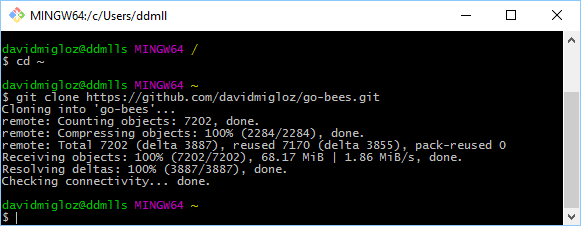
\includegraphics[width=0.9\textwidth]{git-clone}
	\caption{Clonar repositorio de GitHub.}\label{fig:git-clone-1}
\end{figure}

Para conocer el proceso detalladamente consultar \citep{github:clone}.

\subsection{Importar proyecto en Android
Studio}\label{importar-proyecto-en-android-studio}

Una vez obtenido el código fuente de la aplicación, tenemos que
importarlo como proyecto de Android Studio. Para ello, hay que seguir
los siguientes pasos:

\begin{enumerate}
\def\labelenumi{\arabic{enumi}.}
\tightlist
\item
  Abrir Android Studio.
\item
  Menú \texttt{File\ \textgreater{}\ Open\ldots{}}
\item
  Buscamos el directorio donde hemos clonado el repositorio.
\item
  Dentro del repositorio, seleccionamos el archivo
  \texttt{build.gradle}.
\item
  Android Studio detectará que es un proyecto Android y lo importará
  automáticamente.
\item
  Si alguna característica de las que hace uso la aplicación no se
  encuentra instalada, Android Studio mostrará un mensaje de error con
  un enlace para instalar la característica en cuestión.
\end{enumerate}

\begin{figure}[H]
	\centering
	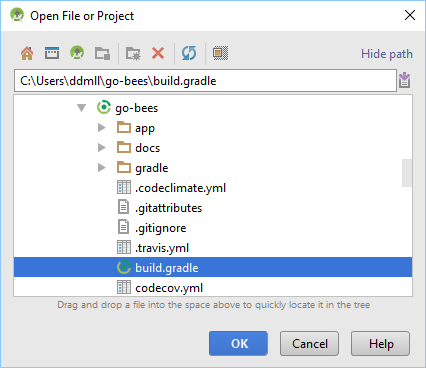
\includegraphics[width=0.4\textwidth]{android-studio-import}
	\caption{Importar proyecto en Android Studio.}\label{fig:android-studio-import}
\end{figure}

Para conocer el proceso detalladamente consultar \citep{android:import}.

\subsection{Añadir nuevas características a la
aplicación}\label{anadir-nuevas-caracteristicas-a-la-aplicacion}

Tras importar el proyecto en Android Studio, ya estamos en disposición
de realizar modificaciones de la aplicación.

Para añadir una nueva característica siguiendo la arquitectura MVP, la
convención de paquete por característica y las metodologías TDD y
GitFlow, se deben seguir los siguientes pasos generales.

\begin{enumerate}
\def\labelenumi{\arabic{enumi}.}
\tightlist
\item
  Crear una nueva rama (\emph{feature branch}) desde la rama
  \emph{develop}:\\
  \texttt{git\ checkout\ -b\ export-data\ develop}
\item
  Crear un nuevo paquete con el nombre de la característica que se desea
  añadir (ej. \texttt{exportdata}).
\item
  Crear una interfaz (ej. \texttt{ExportDataContract.java}) que contenga
  a su vez dos interfaces. En una se deben definir las responsabilidades
  del \emph{presenter} y en la otra las de la vista. Hacer
  \emph{commit}: \\ 
  \texttt{git\ add\ -A} \\
  \texttt{git\ commit\ -m\ "Add\ export\ data\ contract\ \#x"}
\item
  Crear una clase para el \emph{presenter} (ej.\\
  \texttt{ExportDataPresenter.java}) que implemente su correspondiente
  interfaz anterior (no añadir ninguna lógica todavía). Hacer
  \emph{commit}.
\item
  Crear una clase para la vista (ej. \texttt{ExportDataFragment}) que
  descienda de \texttt{Fragment} e implemente su correspondiente
  interfaz anterior (no añadir ninguna lógica todavía). Hacer
  \emph{commit}.
\item
  Crear una clase que descienda de \texttt{AppCompatActivity} (ej. \\
  \texttt{ExportDataActivity.java}) y que enlace el modelo, el
  \emph{presenter} y la vista. Hacer \emph{commit}.
\item
  Crear un test sobre el \emph{presenter} de acuerdo a los requisitos.
  Hacer \emph{commit}.
\item
  Ejecutar el test y comprobar que no pasa.
\item
  Implementar las clases anteriores hasta conseguir que pasen el test.
  Hacer \emph{commit}.
\item
  Refactorizar el código para mejorar su calidad. Hacer \emph{commit}.
\item
  Añadir un \emph{intent} desde donde se quiera acceder a esa
  característica. Hacer \emph{commit}.
\item
  Una vez que se ha implementado correctamente la característica, se
  debe incorporar a la rama \emph{develop} y sincronizar con GitHub:\\
  \texttt{git\ checkout\ develop}\\
  \texttt{git\ merge\ -\/-no-ff\ export-data}\\
  \texttt{git\ branch\ -d\ myfeature}\\
  \texttt{git\ push\ origin\ develop}
\end{enumerate}

\subsection{Actualizar dependencias}\label{actualizar-dependencias}

Una tarea de mantenimiento común es la actualización de las dependencias
de la aplicación. Es importante tenerlas actualizadas para evitar
problemas de seguridad o funcionalidad que pudiesen tener en versiones
anteriores.

El proyecto utiliza Gradle como sistemas de construcción automática del
\emph{software}. Una de sus funcionalidades es la gestión de
dependencias. Esta permite al desarrollador definir las dependencias de
su aplicación, sus versiones y los repositorios donde se hospedan y
Gradle se encarga de descargarlas e importarlas al proyecto
automáticamente.

Las dependencias se definen en el fichero \texttt{build.gradle} del
módulo de la aplicación (\texttt{go-bees/app/build.gradle}):

\begin{figure}[H]
	\centering
	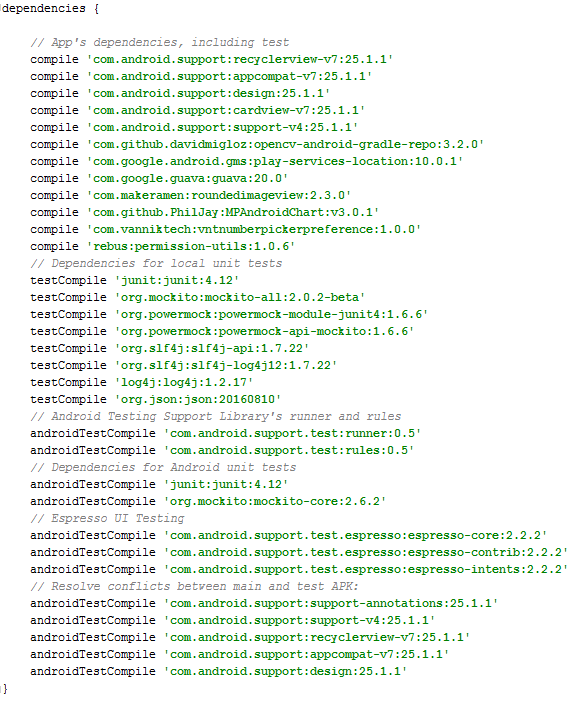
\includegraphics[width=0.8\textwidth]{dependences}
	\caption{Dependencias del proyecto.}\label{fig:dependences}
\end{figure}

Se puede observar que existen tres formas de importar las dependencias,
cada una define con un ámbito de aplicación distinto:

\begin{itemize}
\tightlist
\item
  \texttt{Compile}: estará disponible para el código de la aplicación.
\item
  \texttt{testCompile}: estará disponible en los test unitarios de la
  aplicación.
\item
  \texttt{androidTestCompile}: estará disponible en los test de
  instrumentación de la aplicación.
\end{itemize}

Para actualizar la versión de una dependencia, solamente hay que
actualizar el número de la versión que figura en la importación.
Posteriormente, se debe sincronizar Gradle (\emph{Sync Project with
Gradle Files}).

\subsection{Compilar código fuente}\label{compilar-codigo-fuente}

La compilación del proyecto se realiza mediante la tarea \texttt{build}
de Gradle. Podemos ejecutarla por línea de comandos
(\texttt{./gradlew\ build}) o mediante la interfaz de Android Studio.

\begin{figure}[H]
	\centering
	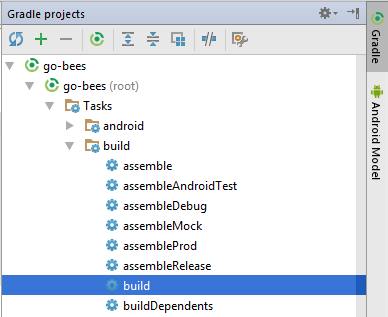
\includegraphics[width=0.5\textwidth]{gradle-build}
	\caption{Compilar proyecto.}\label{fig:gradle-build}
\end{figure}

Todos los ficheros generados durante la compilación se guardan en la
carpeta \texttt{build} del proyecto.

Para conocer el proceso detalladamente consultar
\citep{android:compilerun}.

\subsection{Ejecutar aplicación}\label{ejecutar-aplicacion}

La aplicación se puede ejecutar en un dispositivo real o en un emulador.

\subsubsection{Dispositivo real}\label{dispositivo-real}

Para ejecutar la aplicación en un dispositivo real, se debe conectar
este al equipo de desarrollo mediante un cable USB. El equipo debe tener
los \emph{drivers} del dispositivo instalado, sino no lo reconocerá.

Una vez conectado el dispositivo:

\begin{enumerate}
\def\labelenumi{\arabic{enumi}.}
\tightlist
\item
  Presionar el botón \emph{Run}.
\item
  Si el equipo reconoce el dispositivo se mostrará su nombre debajo de
  ``\emph{Connected Devices}''.
\item
  Seleccionar el dispositivo y pulsa \emph{Ok}.
\item
  Se transferirá el ejecutable de la aplicación y se instalará.
\item
  Una vez instalada, se podrá utilizar la aplicación desde el
  dispositivo.
\end{enumerate}

\subsubsection{Emulador}\label{emulador}

Un emulador (denominados \emph{Android Virtual Device} - AVD) es una
aplicación que simula el funcionamiento de un dispositivo real Android.
La creación y gestión de los emuladores se hace a través de \emph{AVD
Manager}.

Para ejecutar la aplicación en un emulador:

\begin{enumerate}
\def\labelenumi{\arabic{enumi}.}
\tightlist
\item
  Presionar el botón de Run.
\item
  Si ya se posee algún emulador instalado, se mostrará en la lista de
  \emph{Android Virtual Devices}.
\item
  Si no, presionar el botón ``\emph{Create New Virtual Device}''.
\item
  Seleccionar las características que se deseen para el emulador y pulsa
  finalizar.
\item
  Seleccionar el emulador creado y pulsar \emph{Ok}.
\item
  Se iniciará el emulador y se instalará la aplicación en él.
\item
  Una vez instalada, se podrá utilizar la aplicación desde el emulador.
\end{enumerate}

Para conocer el proceso detalladamente consultar
\citep{android:compilerun}.

\subsection{Exportar aplicación}\label{exportar-aplicaciuxf3n}

Para exportar la aplicación como un fichero \texttt{.apk}:

\begin{enumerate}
\def\labelenumi{\arabic{enumi}.}
\tightlist
\item
  Menú \emph{Build} \textgreater{} \emph{Generate APK}.
\item
  Se generará un archivo \texttt{apk} y se guardará en
  \texttt{build/output/apk}.
\end{enumerate}

Si el \texttt{apk} que se desea generar es para distribuirlo en Google
Play, este debe estar firmado. Para ello:

\begin{enumerate}
\def\labelenumi{\arabic{enumi}.}
\tightlist
\item
  Menú \emph{Build} \textgreater{} \emph{Generate Signed APK}.
\item
  Se debe seleccionar el archivo \texttt{.jks} con la clave e introducir
  su contraseña. Si no se dispone de una clave, se puede generar
  siguiendo el asistente.
\item
  Se generará un archivo \texttt{apk} firmado apto para subir al Google
  Play.
\end{enumerate}

Para conocer el proceso detalladamente consultar
\citep{android:compilerun}.

\subsection{Servicios de integración
continua}\label{servicios-de-integracion-continua}

En el repositorio se han integrado varios servicios de integración
continua para detectar fallos en el software lo antes posible,
reduciendo el impacto de estos y aumentando la calidad del código.

A continuación, se describe cada servicio y se indica cómo configurarlo.

\subsubsection{TravisCI}\label{travisci}

TravisCI es una plataforma de integración continua en la nube para
proyectos alojados en GitHub. Permite realizar una \emph{build} del
proyecto y testearla automáticamente cada vez que se realiza un
\emph{commit}, devolviendo un informe con los resultados.

Para integrar Travis en el repositorio hospedado en GitHub se debe crear
una cuenta en su página web y dar permisos de acceso al repositorio. Una
vez asociado el servicio, este se configura mediante el fichero
\texttt{travis.yml}.

Las secciones más importantes de este fichero son:

\begin{itemize}
\tightlist
\item
  \texttt{sudo}: permite definir si el usuario de la máquina virtual
  tendrá privilegios o no.
\item
  \texttt{language}: permite definir el lenguaje de programación del
  proyecto.
\item
  \texttt{jdk}: permite definir la versión del JDK.
\item
  \texttt{compiler}: permite definir el compilador.
\item
  \texttt{addons}: permite configurar \emph{plugins} instalados en
  Travis (como, por ejemplo, el \emph{plugin} de SonarQube).
\item
  \texttt{env}: permite definir variables de entorno.
\item
  \texttt{android}: permite definir las dependencias Android del
  proyecto.
\item
  \texttt{licenses}: permite aceptar las licencias de las dependencias.
\item
  \texttt{before\_install}: en esta sección se pueden definir comandos a
  ejecutar antes de los comandos de la sección \texttt{install} (por ejemplo,
  actualizar la lista de paquetes).
\item
  \texttt{install}: en esta sección se deben definir aquellos comandos
  que instalen alguna dependencia (en nuestro caso
  \texttt{python-numpy}, necesaria para compilar OpenCV).
\item
  \texttt{before\_script}: en esta sección se pueden definir comandos a
  ejecutar antes de la sección script. En nuestro caso, nos descargamos
  el código fuente de OpenCV y lo compilamos.
\item
  \texttt{script}: en esta sección se realiza la compilación del
  proyecto y se ejecutan los diferentes test unitarios y de integración.
  Además, lanza un emulador y ejecuta los test de interfaz. También
  ejecuta el motor de chequeo de SonarQube.
\item
  \texttt{after\_success}: esta sección se utiliza para recolectar datos
  generados en las secciones anteriores. En nuestro caso, se envían los
  diferentes informes de ejecución de los test a el servicio Codecov.
\item
  \texttt{cache}: permite definir los directorios a cachear entre
  ejecuciones.
\end{itemize}

Los \emph{log} de ejecución de Travis son accesibles desde
\citep{travis:gobees}.

\imagen{travis}{TravisCI.}

Para saber más, acceder a su documentación \citep{travis:doc}.

\subsubsection{Codecov}\label{codecov}

Codecov es una herramienta que permite medir el porcentaje de código que
está cubierto por un test. Además, realiza representaciones visuales de
la cobertura y gráficos de su evolución.

La forma de integrarlo en el repositorio es idéntica a cómo se hizo con
Travis. Adicionalmente, hay que configurar el \emph{script} que ejecuta
Travis para que al finalizar su ejecución envíe los resultados a
Codecov.

\texttt{after\_success:\ \ bash\ \textless{}(curl\ -s\ https://codecov.io/bash)}

La configuración de Codecov se define en el archivo
\texttt{codecov.yml}.

\imagen{codecov}{Codecov.}

Para saber más, acceder a su documentación \citep{codecov:doc}.

\subsubsection{CodeClimate}\label{codeclimate}

Codeclimate es una herramienta que realiza revisiones de código
automáticamente.

La integración se realiza de forma similar a Travis. Su fichero de
configuración es \texttt{.codeclimate.yml}.

En nuestro proyecto hemos activado los siguientes motores de chequeo:
\emph{checkstyle}, \emph{fixme}, \emph{markdownlint} y \emph{pmd}.

CodeClimate utiliza el sistema de puntación GPA (\emph{Grade Point
Average}) para indicar el rendimiento general del proyecto. La nota
máxima se corresponde con un 4.0.

Los resultados de los chequeos se encuentran disponibles en
\citep{codeclimate:gobees}.

\imagen{codeclimate}{CodeClimate.}

Para saber más, acceder a su documentación \citep{codeclimate:doc}.

SonarQube es una plataforma de código abierto para la revisión continua
de la calidad de código. Permite detectar código duplicado, violaciones
de estándares, cobertura de test unitarios, \emph{bugs} potenciales,
etc.

Para integrar el servicio hay que seguir los siguientes pasos:

\begin{enumerate}
\def\labelenumi{\arabic{enumi}.}
\tightlist
\item
  Crear una cuenta en
  \href{http://www.sonarqube.com}{www.sonarqube.com}.
\item
  Generar un \emph{token} de autenticación.
\item
  Instalar el plugin de SonarQube para Gradle (\texttt{org.sonarqube}).
\item
  Configurar SonarQube en el fichero de configuración de Gradle
  (\texttt{build.gradle}).
\item
  Ejecutar la nueva tarea sonarqube de Gradle desde Travis.
\end{enumerate}

\imagen{sonarqube-config}{Configuración de SonarQube en Gradle.}

Los resultados de los análisis son accesibles desde
\citep{sonarqube:gobees}.

\imagen{sonarqube}{SonarQube.}

Para saber más, acceder a su documentación \citep{sonarqube:doc}.

\subsubsection{VersionEye}\label{versioneye}

VersionEye es una herramienta que monitoriza las dependencias del
proyecto y envía notificaciones cuando alguna de estas está
desactualizada, es vulnerable o viola la licencia del proyecto.

El servicio se integra de forma similar a Travis. No necesita fichero de
configuración.

Cuando se libera una nueva versión de alguna dependencia o se publica
alguna vulnerabilidad, VersionEye manda una notificación. Se puede
acceder a los informes desde \citep{versioneye:gobees}.

\imagen{versioneye}{VersionEye.}

Para saber más, acceder a su documentación \citep{versioneye:doc}.

\subsubsection{Read the Docs}\label{read-the-docs}

Read the Docs es un servicio de documentación continua que permite crear
y hospedar una página web generada a partir de los distintos ficheros
Markdown o reStructuredText de la documentación. Cada vez que se realiza
un \emph{commit} en el repositorio se actualiza la versión hospedada.

Se integra en el repositorio de la misma manera que Travis. Y se
configura mediante el archivo \texttt{conf.py} ubicado en
\texttt{go-bees/docs/rst}.

Actualmente, se encuentra configurado para generar una sección en la
página web por cada archivo reStructuredText que encuentre dentro del
directorio \texttt{rst}.

\imagen{readthedocs}{Página web generada con ReadTheDocs.}

Para saber más, acceder a su documentación \citep{readthedocs:doc}.

\section{Pruebas del sistema}\label{pruebas-del-sistema}

Para verificar el funcionamiento de cada uno de los módulos de la
aplicación, su integración y la interacción con estos desde la interfaz,
se han desarrollado una serie de baterías de test.

\subsection{Test unitarios}\label{test-unitarios}

Los test unitarios comprueban la funcionalidad de un único módulo
trabajando de forma aislada. Para su escritura se han utilizado las
dependencias jUnit y Mockito.

JUnit es un \emph{framework} de Java utilizado para realizar pruebas
unitarias. Mockito es un \emph{framework} de \emph{mocking} que permite
crear objetos \emph{mock} fácilmente. Estos objetos simulan parte del
comportamiento de una clase. De esta manera, podemos aislar el módulo a
testear para que los módulos de los que depende no interfieran en los
resultados del test.

Se han escrito 120 test unitarios que testean 30 clases distintas. Se
han testeado en su mayoría los \emph{presenters} que son los que poseen
la lógica de la aplicación y no tienen ninguna dependencia al
\emph{framework} de Android. Lo que permite ejecutarlos sin necesidad de
lanzar un emulador.

\imagen{unit-test}{Test unitarios.}

\subsubsection{Ejecución de los test
unitarios}\label{ejecucion-de-los-test-unitarios}

Los test unitarios se ejecutan automáticamente en Travis cada vez que se
realiza un \emph{commit} y se hace un \emph{push} a GitHub. Pero también
se pueden ejecutar en local. Para ello:

\begin{enumerate}
\def\labelenumi{\arabic{enumi}.}
\tightlist
\item
  Seleccionar el \emph{Build Variants} \texttt{mockDebug}.
\item
  Seleccionar como tipo de vista Android.
\item
  Pulsar botón derecho en el paquete \texttt{test} \textgreater{}
  \emph{Run test in go-bees.}
\item
  Se ejecutarán todos los test y se obtendrá un informe de resultados.
\end{enumerate}

\imagen{run-unit-test}{Ejecución de los test unitarios.}

\subsection{Test del algoritmo}\label{test-del-algoritmo}

Para testear el algoritmo se han escrito varios test unitarios que
prueban cada uno de sus módulos y un test de integración
(\texttt{AreaBeesCounterTest.java}) que lo testea en su totalidad contra
tres conjuntos de fotogramas etiquetados manualmente. De esta manera, se
obtiene el error que comete el algoritmo en cada caso y se compara con
unos límites prefijados. Si por alguna modificación accidental el error
supera el límite, el test falla.

\subsubsection{Ejecución del test del
algoritmo}\label{ejecucion-del-test-del-algoritmo}

El test de integración se ejecuta automáticamente en Travis junto con
los test unitarios. También puede ser ejecutado en local, pero es
imprescindible tener instalado OpenCV en el equipo. Los pasos a seguir
son:

\begin{enumerate}
\def\labelenumi{\arabic{enumi}.}
\tightlist
\item
  Seleccionar el \emph{Build Variants} \texttt{mockDebug}.
\item
  Seleccionar como tipo de vista Android.
\item
  Pulsar botón derecho en el paquete \texttt{testMock} \textgreater{}
  \emph{Run test in go-bees.}
\item
  Se ejecutará el test y se obtendrá un informe de resultados.
\end{enumerate}

\imagen{algo-test}{Ejecución del test de integración del algoritmo.}

\subsubsection{Etiquetado de nuevos conjuntos de
fotogramas}\label{etiquetado-de-nuevos-conjuntos-de-fotogramas}

Para etiquetar videos manualmente se ha desarrollado una aplicación en
Java que facilita esta labor. La aplicación va mostrando cada fotograma
y el usuario solo tiene que pinchar encima de cada abeja existente.
Finalmente, la aplicación permite exportar los datos en un archivo
\texttt{CSV} con el formato que utiliza el test del algoritmo.

Los pasos a seguir son:

\begin{enumerate}
\def\labelenumi{\arabic{enumi}.}
\tightlist
\item
  Ejecutar la aplicación (Disponible en \citep{github:extraapps}).
\item
  Abrir el directorio que posee los fotogramas.
\item
  Marcar las abejas presentes en cada fotograma con el ratón. La
  aplicación mostrará el número del fotograma y el número de abejas
  marcadas.
\item
  Al finalizar, seleccionar guardar. La aplicación exportará los datos
  en un archivo \texttt{CSV}.
\end{enumerate}

\imagen{counting_platform}{Aplicación de etiquetado de fotogramas.}

\subsubsection{Testeo de la parametrización del
algoritmo}\label{testeo-de-la-parametrizacion-del-algoritmo}

Para desarrollar el algoritmo y parametrizarlo de forma óptima, se
desarrolló una aplicación Java que permite modificar los diferentes
parámetros de cada fase en tiempo real y calcular sus tiempos de
cómputo.

Si se desea probar nuevas parametrizaciones:

\begin{enumerate}
\def\labelenumi{\arabic{enumi}.}
\tightlist
\item
  Ejecutar la aplicación (Disponible en \citep{github:extraapps}. Es
  necesario tener instalado OpenCV en el equipo).
\item
  Seleccionar un archivo de vídeo de prueba.
\item
  En la ventana izquierda se visualiza la entrada del algoritmo y a la
  derecha existe una pestaña por cada fase de este.
\item
  En cada pestaña, a parte de la salida del algoritmo para esa fase, se
  poseen una serie de controles para parametrizar el algoritmo.
\item
  En la parte inferior izquierda se muestra los fotogramas por segundo
  que se están procesando. En la parte central, el tiempo total de
  procesado. Y en la parte derecha, el tiempo parcial de la fase en
  cuestión.
\end{enumerate}

\imagen{devplatform}{Plataforma de desarrollo del algoritmo.}

\subsection{Test de interfaz}\label{test-de-interfaz}

Por último, se han desarrollado 17 test de interfaz que testean cada uno
de los requisitos de la aplicación, a excepción del requisito de
monitorización que no fue posible testearlo en un emulador (no se puede
utilizar como \emph{feed} de la cámara de un emulador un archivo de
vídeo).

Para desarrollar los test se ha utilizado Espresso, un \emph{framework}
de \emph{testing} para Android que provee una API para escribir UI test
que simulen las interacciones de usuario con la \emph{app}.

En la siguiente tabla se relaciona cada test con el requisito que
comprueba.

\begin{table}[H]
\centering
\begin{tabular}{ll}
\toprule
Test                     & Requisitos                           \\
\midrule
\texttt{AddApiaryTest.java}       & RF-1.1 Añadir colmenar.              \\
\texttt{EditApiaryTest.java}      & RF-1.2 Editar colmenar.              \\
\texttt{DeleteApiaryTest.java}    & RF-1.3 Eliminar colmenar.            \\
\texttt{ListApiariesTest.java}    & RF-1.4 Listar colmenares.            \\
\texttt{ViewApiaryTest.java}      & RF-1.5 Ver colmenar.                 \\
\texttt{AddHiveTest.java}         & RF-2.1 Añadir colmena.               \\
\texttt{EditHiveTest.java}        & RF-2.2 Editar colmena.               \\
\texttt{DeleteHiveTest.java}      & RF-2.3 Eliminar colmena.             \\
\texttt{ListHivesTest.java}       & RF-2.4 Listar colmenas.              \\
\texttt{ViewHiveTest.java}        & RF-2.5 Ver colmena.                  \\
\texttt{AddRecordingTest.java}    & RF-3.1 Añadir grabación.             \\
\texttt{DeleteRecordingTest.java} & RF-3.2 Eliminar grabación.           \\
\texttt{ListRecordingsTest.java}  & RF-3.3 Listar grabaciones.           \\
\texttt{ViewRecordingTest.java}   & RF-3.4 Ver grabación.                \\
\texttt{SettingsTest.java}        & RF-5 Configuración de la aplicación. \\
\texttt{HelpTest.java}            & RF-6 Ayuda de la aplicación.         \\
\texttt{AboutTest.java}           & RF-7 Información de la aplicación.  \\
\bottomrule
\end{tabular}
\caption{Requisitos testeados.}
\label{requisitos-test}
\end{table}

\subsubsection{Ejecución de los test de
interfaz}\label{ejecucion-de-los-test-de-interfaz}

Para ejecutar los test de interfaz es imprescindible contar con un
dispositivo físico o un emulador. Una vez conectado, se siguen los
siguientes pasos:

\begin{enumerate}
\def\labelenumi{\arabic{enumi}.}
\tightlist
\item
  Seleccionar el \emph{Build Variants} \texttt{mockDebug}.
\item
  Seleccionar como tipo de vista Android.
\item
  Pulsar botón derecho en el paquete \texttt{androidTest} \textgreater{}
  \emph{Run test in go-bees.}
\item
  Se ejecutarán cada uno de los test en el dispositivo (Android Studio
  instala una aplicación adicional que instrumenta a la aplicación a
  testear).
\item
  Al finalizar, se obtiene un informe con los resultados.
\end{enumerate}

\apendice{Documentación de usuario}

\section{Introducción}

\section{Requisitos de usuarios}

\section{Instalación}

\section{Manual del usuario}





\bibliographystyle{plain}
\bibliography{bibliografiaAnexos}

\end{document}